%\iffalse
% -----------------------------------------------------------------
% File:       dgruyter.dtx
% Author:     le-tex publishing services
% Maintainer: le-tex publishing services
%
% This file is part of the dgruyter package for preparing
% books for Walter de Gruyter GmbH.
%
%       Copyright (C) 2015, 2016, 2017, 2018 Walter de Gruyter GmbH
%
% -----------------------------------------------------------------
% This file contains the documentations and source code for the
% dgruyter package for use with LaTeX2e. See the file 'README'
% for a list of all the files as well as directions for the
% installation of this package.
% -----------------------------------------------------------------
%<*driver>
\ProvidesFile{dgruyter.dtx}
%</driver>
%<package>\NeedsTeXFormat{LaTeX2e}[2014/05/01]
%<package>\ProvidesPackage{dgruyter}
%<*package>
    [2017/09/19 v2.00 De Gruyter layout]
%</package>
%<*driver>
\documentclass[a4paper]{ltxdoc}
  \frenchspacing
  \parindent0pt
  \parskip\medskipamount
  \makeatletter
  \def\@listi{\leftmargin\leftmargini
              \parsep\z@
              \topsep\z@
              \itemsep\z@}
  \let\@listI\@listi
  \@listi
  \def\@listii{\leftmargin\leftmarginii
              \labelwidth\leftmarginii
              \advance\labelwidth-\labelsep
              \parsep\z@
              \topsep\z@
              \itemsep\z@}
  \makeatother
  \emergencystretch1em
  \clubpenalty10000
  \widowpenalty10000
  \def\hack#1{#1}
  \RequirePackage[T1]{fontenc}
  \RequirePackage[utf8]{inputenc}
  \RequirePackage{color}
  \RequirePackage{graphicx}
  \RequirePackage{lmodern}
  \IfFileExists{DGMetaSerifScience.sty}
    {\RequirePackage{DGMetaSerifScience}}
    {}
  \RequirePackage[breaklinks,pdfborder={0 0 0}]{hyperref}
  \DisableCrossrefs
  \OnlyDescription
\begin{document}
  \DocInput{dgruyter.dtx}
\end{document}
%</driver>
%\fi
%
% \CheckSum{7998}
% \CharacterTable
%    {Upper-case    \A\B\C\D\E\F\G\H\I\J\K\L\M\N\O\P\Q\R\S\T\U\V\W\X\Y\Z
%     Lower-case    \a\b\c\d\e\f\g\h\i\j\k\l\m\n\o\p\q\r\s\t\u\v\w\x\y\z
%     Digits        \0\1\2\3\4\5\6\7\8\9
%     Exclamation   \!     Double quote  \"     Hash (number) \#
%     Dollar        \$     Percent       \%     Ampersand     \&
%     Acute accent  \'     Left paren    \(     Right paren   \)
%     Asterisk      \*     Plus          \+     Comma         \,
%     Minus         \-     Point         \.     Solidus       \/
%     Colon         \:     Semicolon     \;     Less than     \<
%     Equals        \=     Greater than  \>     Question mark \?
%     Commercial at \@     Left bracket  \[     Backslash     \\
%     Right bracket \]     Circumflex    \^     Underscore    \_
%     Grave accent  \`     Left brace    \{     Vertical bar  \|
%     Right brace   \}     Tilde         \~}
%
% \GetFileInfo{dgruyter.dtx}
% 
% \title{The \texttt{dgruyter} Package\,\thanks{This package was created by le-tex publishing
% services, Leipzig for Walter de Gruyter, Berlin.\hfil\break\hspace*{1.8em}This file has version
% number \fileversion, last revised \filedate.}}%
% \author{Walter de Gruyter GmbH}%
% \date{Printed \today}%
% 
% \maketitle
% \tableofcontents
% 
%
% \section{Introduction}\label{sec:intro}
%
% The \texttt{dgruyter} package assists in preparing manuscripts for De\,Gruyter with {\LaTeX}. It
% provides some special commands for journal articles as well as for books and generates the
% required appearance. Together with corresponding font packages it allows to produce the final
% layout of De\,Gruyter books and journal articles.
%
% The |README| file describes the installation of the package.
% 
% The \texttt{dgruyter} package consists of the following files:
% \begin{description}
% \item[\texttt{dgruyter.sty}] the {\LaTeX} package file
% \item[\texttt{dgruyter.pdf}] this documentation
% \item[\texttt{dgruyter.ist/.xdy}] index style files (for \texttt{Makeindex} and \texttt{Xindy}, respectively)
% \item[\texttt{DG\_attention.eps/.pdf,}] \texttt{\bfseries DG\_exercise.eps/.pdf},
%   \texttt{\bfseries DG\_information.eps{\slash}.pdf}, \texttt{\bfseries DG\_notice.eps/.pdf},
%   \texttt{\bfseries DG\_question.eps/.pdf} vignette files (for special environments)
% \item[\texttt{dg-degruyter.eps/.pdf, dg-mouton.eps/.pdf, dg-saur.eps/.pdf}] logo files (for the
%   main title page of a book)
% \item[\texttt{book.tex}] a {\LaTeX} master file for a book, to be used as a template
% \item[\texttt{journal-article.tex}] a {\LaTeX} master file for an article, to be used as a template
% \end{description}
%
% Note that the final layout will require the non-standard fonts DG\,Meta and MinionMath. These
% fonts come with extra packages that have to be installed separately from the \texttt{dgruyter}
% package. Please ask your De\,Gruyter contact if you need more information. |dgruyter.sty| itself
% checks whether these fonts are installed in your {\TeX} distribution, otherwise it switches to
% the standard {\LaTeX} font (Latin\,Modern). That is, the \texttt{dgruyter} package works
% without DG\,Meta and MinionMath as well.
%
% This documentation is not intended to give an introduction to {\LaTeX}.  For questions concerning
% {\TeX} systems/installations or the {\LaTeX} mark-up language in general please visit
% \url{www.tug.org}, \url{www.dante.de}, \url{uk.tug.org} or any other {\TeX} user group
% worldwide. The essential reference for {\LaTeX} is \emph{Mittelbach~F., Goossens~M. (2004) The
% {\LaTeX} Companion. 2nd edn.}, but there are many other good books providing insight into
% {\LaTeX}.
%
% \texttt{dgruyter} tries to benefit from standard {\LaTeX} packages.  (Have a look at
% |dgruyter.sty| to see which packages are used.)  To learn more about the underlying packages we
% refer to their documentations (try for instance ``|texdoc [package name]|'' at your shell prompt or
% visit \url{tug.ctan.org}).
%
%
% \section{General usage}
%
% We suggest to employ a recent {\TeX} installation: the most important distributions, {\TeX}\,Live,
% MiK{\TeX}/pro{\TeX}t, and Mac{\TeX}, all provide at least 2015 versions. But older versions should
% (in principle) work as well.
%
% To use the \texttt{dgruyter} package, put the files mentioned above in your working directory,
% edit the file |article.tex| or |book.tex| in your preferred text editor and run {\LaTeX} as usual.
% (See the following section for more detailed advises.)
%
%
% \section{Some important settings and package features}\label{sec:usage}
%
% \subsection{Options for the document class}
%
% {\LaTeX}'s article class or book class know several options.
%
% The following class options should \textit{not} be used together with |dgruyter.sty|: |a4paper|,
% |a5paper|, |b5paper|, |letterpaper|, |legalpaper|, |executivepaper|, |landscape|, |10pt|, |11pt|,
% |12pt|, |oneside|, |twoside|, |titlepage|, |notitlepage|, |leqno|, |fleqn|, and
% |openbib|. (Corresponding settings are done by |dgruyter.sty| itself.)
%
% The following class options, however, might be used: |draft|, |final|, |onecolumn|, |twocolumn|,
% |openright|, and |openany|.
%
% Because |dgruyter.sty| already loads the \texttt{babel} package it is recommended to provide a language
% option together with |\documentclass|. Suitable language options are, e.g., |Ukenglish|,
% |USenglish|, or |ngerman|. (Note that |dgruyter.sty| itself passes |english| as a kind of
% fallback language to the \texttt{babel} package, anyhow.)
%
% \subsection{Engines, encoding packages, and fonts}
%
% The \texttt{dgruyter} package does not prescribe the {\TeX} engine to be used. The standard engine
% nowadays is |pdfTeX|; a recent alternative is |luaTeX|.
%
% With the standard engine |pdfTeX|, one can choose between different output and input
% encodings. Output encodings are selected with the \texttt{fontenc} package.  |dgruyter.sty|
% already pre-loads the standard encoding |T1|. To provide further encodings, add to the {\LaTeX}
% preamble:
% \begin{verbatim}
% \usepackage[<encoding-options>]{fontenc}
% \end{verbatim}
% \vskip-\baselineskip
% One might also choose an input encoding other than the default ASCII encoding by adding
% \begin{verbatim}
% \usepackage[<encoding-option>]{inputenc}
% \end{verbatim}
% \vskip-\baselineskip to the {\LaTeX} preamble. For example, for the recommended UTF-8 encoding,
% choose the option |utf8|.
%
% The modern |luaTeX| engine has a different approach to handle encodings: It uses Unicode/UTF-8 as
% a default. So, in general no encoding settings (via package loading) are required.\\
% The standard package to use fonts with |luaTeX| is the \texttt{fontspec} package. To use this, add
% something like |\usepackage[no-math]{fontspec}| to your preamble. (The alternative
% |XeTeX| engine works similar.)\\
% If the \texttt{fontspec} package is loaded, the math fonts will be set-up with the
% \texttt{unicode-math} package.
%
% Please load the packages \texttt{fontenc}, \texttt{inputenc}, or \texttt{fontspec} before loading
% |dgruyter.sty| itself.
%
% As already mentioned, |dgruyter.sty| checks whether the specific De\,Gruyter fonts are
% installed and acts accordingly. More precisely:
% \begin{itemize}
% \item If the \texttt{fontspec} package is not loaded (as is the case with standard |pdfTeX|), it
%   checks whether a file |DGMetaSerifScience.sty| exists. If it exists, it presumes that the fonts
%   DG\,Meta\,Science and DG\,MetaSerif\,Science are installed through the respective packages from
%   De\,Gruyter (otherwise errors will result). Then it loads the math font ``MinionMath'' if it is
%   installed through |minionmath.sty|.
% \item If \texttt{fontspec} is loaded, |dgruyter.sty| looks for DGMetaScience OpenType font files
%   and loads them if present. Afterwards it proceeds similarily with the MinionMath font.
% \end{itemize}
%
% \subsection{The \texttt{dgruyter} package and its options}
%
% To use the \texttt{dgruyter} package, add |\usepackage[<options>]{dgruyter}| to your {\LaTeX}
% preamble.
%
% |dgruyter.sty| knows two option groups: layout-format options and mode options.
%
% \subsubsection{Layout-format options}
%
% Format options specify the layout size of your document.
% \begin{description}
% \item[\hbox to3.5em{\texttt{small}}] $155\times 230\,\mathrm{mm}$
% \item[\hbox to3.5em{\texttt{medium}}] $170\times 240\,\mathrm{mm}$ (only available for books)
% \item[\hbox to3.5em{\texttt{big}}] $210\times 280\,\mathrm{mm}$
% \end{description}
% The |big| layout is (mostly) a two-column layout.
%
% Note that exactly one one of these format option must be provided.  Please ask your De\,Gruyter
% contact which one to choose.
%
% The additional format option |margincol| is to adapt the layout in favour of a margin column. Margin
% notes can be added with |\marginpar| as usual.
%
% \subsubsection{Mode options}
%
% Mode options specify the output mode.\nopagebreak
% \begin{description}\nopagebreak
% \item[\texttt{online \mdseries<default>}] produces the document optimised for screen reading, i.e., with the
%   final page format, hyperlinks and bookmarks.
% \item[\texttt{print}] produces the document optimised for printing, i.e., hyperlinks and bookmarks
%   are switched off. 
% \iffalse\item[\texttt{printona4}] puts th page on an DIN\,A4 sheet with crop marks and a
%   document info line; the TrimBox is set.\fi
% \item[\texttt{work}] produces the document as in online mode but additionally with a layout frame for the
%   type-area that simplifies manual type-setting and page-breaking.
% \end{description}
% In general, the final document is to be delivered in |print| mode.
%
% \subsection{Symbols for IPA}
%
% The \texttt{tipa} package is preloaded. Note that this is done with the option |safe| in order to retain
% normal behaviour of |\!| and similar commands in math mode.
%
% \subsection{Formulae}
%
% According to the De\,Gruyter style guide lines, displayed formulae should be centred and equation
% numbers must be at the right margin, so do \textit{not} use the |fleqn| option (for equations
% aligned left) or the |leqno| option (for equation numbers on the left), either.
%
% The \texttt{amsmath} package is preloaded, and your are encouraged to use its mark-up like the
% |\frac{}{}| command or the |{align}| environment instead of old-style mark-up like the |\over| command or the |{eqnarray}|
% environment.
%
% \subsection{Theorem-like environments}
%
% Through the \texttt{amsthm} package, |dgruyter.sty| provides two theorem styles: |dgdef| (upright
% text body) and |dgthm| (text body in italics). Please use these styles to introduce new
% theorem-like environments with the |\theoremstyle| and |\newtheorem| commands.
%
% \subsection{Text boxes}\label{sec:el:box}
%
% The \texttt{dgruyter} package provides the new |{note}| environment for
% highlighted text passages. |{note}| will display its content between
% two horizontal rules. The environment provides an optional argument
% to add a vignette in the margin. Write, e.g.,
% \begin{verbatim}
% \begin{note}[DG_attention]
%   This is a special box.
% \end{note}
% \end{verbatim}
% \vskip-\baselineskip%
% to add the ``attention'' vignette. The following vignettes can be used in your document:\\
% |DG_attention| -- \lower0.5ex\hbox{
\includegraphics{logos/DG_attention}}, |DG_exercise| --
% \lower0.5ex\hbox{
\includegraphics{logos/DG_exercise}}, |DG_information| --
% \lower0.5ex\hbox{
\includegraphics{logos/DG_information}}, |DG_notice| --
% \lower0.5ex\hbox{
\includegraphics{logos/DG_notice}}, and |DG_question| --
% \lower0.5ex\hbox{
\includegraphics{logos/DG_question}}.
%
% \subsection{Graphics}
%
% The standard interface for graphic inclusion is the |\includegraphics| command provided by the
% \texttt{graphicx} package (which is also preloaded). Use the package option ``|draft|'' to
% (temporarily) switch off graphic inclusion (this may save processing time when generating
% PostScript or PDF output). Note that the |\graphicspath| command allows to declare one or more
% folders where the \texttt{graphicx} package looks for the image files, therefore it is not
% necessary to type in the whole file path into each |\includegraphics| command.
%
% \subsection{Tables}
%
% Preloaded packages are: the \texttt{array} package (for introducing new column types), the
% \texttt{multirow} package (row spanning cells), the \texttt{tabularx} package (automatic column
% width calculation), and the \texttt{supertabular} package (multi-page tables).
%
% Because the table layout requires horizontal rules but forbids vertical rules, the \texttt{booktabs}
% package is also preloaded.  The required horizontal rules at the top and at the bottom of the
% tabular material will be inserted automatically. To separate the table head and the table body,
% use the |\midrule| command \textit{after} the |\\| of your table's last heading line: It generates
% an additional rule and will also switch from the tabular head font to the tabular body font. For
% tables without header add |\starttabularbody| immediately after
% |\begin{tabular}{...}|.\iffalse\end{tabular}\fi
%
% There is a switch |\baretabulars| to return to LaTeX's standard look\,\&\,feel for
% tabulars. Respectively, |\layouttabulars| reactivates the required tabular layout. (Note that
% these switches act locally).
%
% \subsection{Floats}
%
% Captions of figures, tables, etc. are generated with the help of the \texttt{caption} package.
%
% For narrow floating images (i.e. images whose widths are equal or less than half of the text
% width) it is recommended to place the caption besides the object. To achieve this, the preloaded
% \texttt{sidecap} package provides the environment |{SCfigure}|. Please do not use the |SC|
% environments if the resulting caption will need more vertical space than the object itself.
%
% \subsection{Rotating floats}
%
% The preloaded \texttt{rotating} package provides the two environments ``|sidewaysfigure|'' and
% ``|sidewaystable|''. They allow the rotation of floating objects.
%
% \subsection{Linguistic structures}\iffalse Maria.Dassing@degruyter.com\fi
%
% To produce linguistic structures, one can use the common packages together with
% |dgruyter.sty|. For example, to create examples with labeled parts or interlinear glosses, try one
% of the packages:
% \begin{itemize}
% \item \texttt{gb4e} (preferably followed by |\noautomath|)
% \item \texttt{linguex}
% \item \texttt{expex}
% \end{itemize}
% (In case of doubt, load the packages \emph{after} |dgruyter.sty|.)
%
% \subsection{Scholary editions with the \texttt{reledmac} package}
%
% |dgruyter.sty| is compatible with the \texttt{reledmac} package. But note that it has to be loaded
% before the \texttt{reledmac} package.
%
% \subsection{Source code}\iffalse Maria.Dassing@degruyter.com\fi
%
% To capture computer code, the \texttt{listings} package is a good option. Please see the
% \texttt{listings} documentation for further information on usage and configuration, e.g. how to
% use the |\lstset{...}| command for parameter settings. Note that the \texttt{dgruyter} package
% pre-configures the \texttt{listings} package to use a typewriter font and espcially the
% |lstlisting| environment to have left-hand line numbers in the type area and not in the margin;
% the width of the line-number column can be fine-tuned with the known |numbersep| key from the
% \texttt{listings} package.
%
% \subsection{Bibliography}
%
% It is recommended to use the standard bibliography mechanism. You might copy and paste your
% bibliography entries from elsewhere into the |thebibliography| environment or, more elegantly, use
% \textsc{Bib}{\TeX}. The \texttt{dgruyter} package does not prescribe any particular bibliography
% style.
%
% The \texttt{natbib} package can be loaded additionally, so an author-year-style bibliography
% layout is possible. The special citing commands |\citet|, |\citep| and so on can be used. Feel
% free to configure \texttt{natbib}, e.g. with |\setcitestyle{numbers}| in your document preamble to force
% the numerical mode.
%
% Alternatively, the \texttt{biblatex} package can be used. Be aware, however, that there is an
% abundance of options which have not all been tested for compatibility with the |dgruyter|
% package. The following seem to work fine for the numeric style:
% \begin{itemize}
% \item |\usepackage[backend=bibtex]{biblatex}|\quad to load the package,
% \item |\addbibresource{BIBFILE}|\quad\quad to load the .bib-file,
% \item |\printbibliography[env=bibnumeric]|\quad\quad\ \  to output the bibliography.
% \end{itemize}
% With author-year citation you have to skip the optional argument of\break |\printbibliography|.
%
% \subsection{Index}
%
% The traditional tool for index generation is \texttt{Makeindex}. The
% \texttt{dgruyter} package provides the \texttt{Makeindex} style file ``\texttt{dgruyter.ist}''. To
% use \texttt{Makeindex} type, e.g.
% \begin{verbatim}
% makeindex -c -s dgruyter.ist book
% \end{verbatim}
% \vskip-\baselineskip%
% If you need a more elaborate index generation tool (e.g. for better alphabetical sorting in German
% books) you might prefer the program ``\texttt{Xindy}''. The corresponding style file is
% \texttt{dgruyter.xdy}. To use \texttt{Xindy} type, e.g.,
% \begin{verbatim}
% texindy -M dgruyter book.idx
% \end{verbatim}
% \vskip-\baselineskip or for German books
% \begin{verbatim}
% texindy -g -M dgruyter book.idx
% \end{verbatim}
% \iffalse texindy -M lang/general/utf8 -M dgruyter book.idx\fi
%
%
% \section{Journal articles}
%
% The \texttt{dgruyter} package is designed to produce journal articles as well as whole books. In
% this section, some features concerning journal articles are discussed; the following section will
% then give some special advise concerning books.
%
% All the explanations given so far hold, in particular, for journal articles. Here, some
% information concerning (1)~the article header and (2)~the end of an article are added. In
% addition, (3)~some special structures for journals material beyond individual articles are
% commented.
%
% To use the \texttt{dgruyter} package for a journal article, it is necessary to employ {\LaTeX}'s
% |article| document class.
%
% \subsection{The article header}\label{sec:Arthead}
%  
% In a {\LaTeX} article it is common to first provide some title and meta information and then call
% the |\maketitle| command to process and output all this information. The same holds when
% |dgruyter.sty| is active. Here are the user macros one can/must use to provide article-specific
% information before calling |\maketitle|:
% \begin{description}
% \item[|\textbackslash articletype\{...\}|] For an article type like ``|Editorial|''; it will be
%   rendered at the top of the header.
% \item[|\textbackslash articlesubtype\{...\}|] For an article subtype like ``|Research Article|''; it will be
%   rendered under the article type.
% \item[|\textbackslash openaccess|] To mark an article with ``Open Access''; it will be rendered in
%   the right upper corner.
% \item[|\textbackslash author\char"5B...\char"5D\{...\}|] For the author name. The |author| command can be
%   used as with the \texttt{authblk} package, that is, it can occur more than once. The optional argument can be
%   added to refer to a corresponding |\affil{...}| command, and besides that one can use the starred version,
%   |\author*{...}|, to mark the author as the corresponding author.
% \gdef\docAFFIL{\item[|\textbackslash affil\char"5B...\char"5D\{...\}|] For an affiliation; the syntax is as with
%   the \texttt{authblk} package. Note that an optional e-mail address should be added after the actual
%   affiliation, like: |\char"5Caffil\{Institute ..., University ..., e-mail: johnq.public@inst.org\}|.}\docAFFIL
% \gdef\docRUNNINGAUTHOR{\item[|\textbackslash runningauthor\{...\}|] This optional macro is to provide author names
%   specifically for the running header, e.g. |\char"5Crunningauthor\{John Q. Public et al.\}|.}\docRUNNINGAUTHOR
% \item[|\textbackslash title\{...\}|] For the title of the article.\footnote{You can add notes to
%   the title\iffalse, either using \texttt{\textbackslash footnote} (or rather \texttt{\textbackslash
%   footnotemark} plus \texttt{\textbackslash footnotetext in two-column articles}), or\fi{} using
%   \texttt{\textbackslash articlenote} (in two-column mode, please put \texttt{\textbackslash
%   articlenote} outside the column-spanning title area, e.g. in the abstract).}%
%   \gdef\docRUNNINGTITLE{\item[|\textbackslash runningtitle\{...\}|] This optional macro is to
%   provide a specific (shorter) title for the running header.}\docRUNNINGTITLE
% \item[|\textbackslash subtitle\{...\}|] For an optional sub-title of the article.
% \gdef\docABSTRACT{\item[|\textbackslash abstract\{...\}|] For the abstract.}\docABSTRACT
% \gdef\docKEYWORDS{\item[|\textbackslash keywords\{...\}|] For key words.}\docKEYWORDS
% \gdef\docABSTRACTTRANS{\item[|\textbackslash transabstract\char"5B...\char"5D\{...\}|] For a translated abstract. 
%   The optional argument is to specify a language (in babel style).}\docABSTRACTTRANS
% \gdef\docKEYWORDSTRANS{\item[|\textbackslash transkeywords\char"5B...\char"5D\{...\}|] For translated key words.
%   The optional argument is to specify a language (in babel style).}\docKEYWORDSTRANS
% \gdef\docCORRECTIONNOTE{\item[|\textbackslash correctionnote\char"5B...\char"5D\{...\}|] For an erratum/corrigendum/retraction.
%   The optional argument is to provide an alternative heading string.}\docCORRECTIONNOTE
% \gdef\docCLASSIFICATION{\item[|\textbackslash classification\char"5B...\char"5D\{...\}|] For classification information. The
%   optional argument is to provide a classification system (e.g. |MSC|, |PACS|, or |JEL|).}\docCLASSIFICATION
% \item[|\textbackslash communicated\{...\}|] For the person who ``communicated'' the paper.
% \item[|\textbackslash dedication\{...\}|] For a dedication.
% \item[|\textbackslash received\{...\}|] For the ``received'' date, e.g. |\received{May 19, 2013}|.
% \item[|\textbackslash accepted\{...\}|] For the ``accepted'' date, e.g. |\accepted{June 30, 2013}|.
% \item[|\textbackslash journalname\{...\}|] For the (abbreviated) journal name,\hack{\\} e.g. |\journalname{Biol. Chem.}|.
% \item[|\textbackslash journalyear\{...\}|] For the year (default is the present year).
% \item[|\textbackslash journalvolume\{...\}|] For the journal volume.
% \item[|\textbackslash journalissue\{...\}|] For the journal issue.
% \item[|\textbackslash startpage\{...\}|] For the article's start page.
% \item[|\textbackslash aop|] A switch that activates output of ``|; aop|'' (i.e. ``ahead of
%   print'') and, at the same time, suppresses output of the journal volume, the journal issue, and
%   the article's page range.  \gdef\docDOI{\item[|\textbackslash DOI\{...\}|] For the DOI of the
%   paper.}\docDOI%
%   \gdef\doccontributioncopyright{\item[|\textbackslash
%   contributioncopyright\char"5B...\char"5D\{...\}\{...\}\{...\}|] For copyright information in
%   case De\,Gruyter does not solely hold the copyright or the work is an open access
%   publication. The optional argument expects the name of an image file, usually a Creative Commons
%   logo. The three obligatory arguments are for the copyright year, the copyright holder (and
%   a possible publisher addition), and a copyright text (e.g. a Creative Commons text),
%   respectively.}%
%   \doccontributioncopyright
% \end{description}
% The contents of |\journalname{...}| and the subsequent macros will be rendered in the running
% header of the article's start page.
% 
% As already mentioned, all this information will be output by invoking the |\maketitle| command.
%
% \subsection{At the end of an article}
%  
% At the end of an article, there are three special environments that can be used:
% |{acknowledgement}|, |{funding}|, |{conflictofinterest}|. They should be placed before the
% bibliography.
% \begin{description}
% \item[|\textbackslash articlenote\{...\}|] A container for pre-publication information or for
%   information about the content or about supplemental material. It should only be used at the end
%   of the article. For example, use \\
%   |\articlenote{%|\\
%   |    \textbf{Supplemental Material:} The online version ...\\|\\
%   |    \textbf{Note:} This ...}|.%
% \end{description}
%
% \subsection{Some journal-specific macros beyond individual articles}
%  
% \subsubsection{Graphical abstracts}
%
% The |{thegraphicalabstractsection}| environment sets up the layout for a section with graphical
% abstracts. Inside this environment a list of |\graphicalabstract| commands should be given.
%
% \goodbreak|\graphicalabstract| has five obligatory arguments:\nopagebreak
% \begin{description}\nopagebreak
% \item[|\#1|] the author's names
% \item[|\#2|] the article's title
% \item[|\#3|] the article's meta information (DOI, journal name)
% \item[|\#4|] the abstract
% \item[|\#5|] file name of an image
% \end{description}\enlargethispage{\baselineskip}
%
% \subsubsection{List of contributors}
%
% The |{contributors}| environment sets up the layout for a section contributors. The environment
% has one optional argument to overwrite the default title (``List of contributors''). Inside this
% environment a list of |\contributor| commands should be given.
%
% |\contributor| has five obligatory arguments:
% \begin{description}
% \item[|\#1|] the contributor's name
% \item[|\#2|] the contributor's address
% \item[|\#3|] the contributor's e-mail address
% \item[|\#4|] file name of a contributor's picture
% \item[|\#5|] a short vita
% \end{description}
%
% \subsubsection{Reviews}
%
% For reviews, two additional macros are provided, |\reviewauthor| and |\reviewinfo|. They should be
% used as shown in the following example:
% \begin{verbatim}
% \articletype{Buchrezension}
% \reviewauthor{Peter Rezensent}
% \affil{Universität Muster, Musterstraße 3, 11111 Stadt,
%    E-Mail: paul@muster.de}
% \title{Die Kraft der Kunst}
% \DOI{10.1515/dzph-2013-0002}
% \reviewinfo{\textbf{Erika Mustermann:} Die Kraft der Kunst, Suhrkamp 2012}
% \maketitle
% Lorem ipsum ...\par
% \articlenote{[additional information]}
% \end{verbatim}
%
% Further reviews can be added with the |\furtherreview| macro (four arguments), e.g.:
% \begin{verbatim}
% \furtherreview
%   {\textbf{Erika Mustermann:} Die Kraft der Kunst, Suhrkamp Verlag 2012}
%   {Peter Rezensent}
%   {Universität Muster, Musterstraße 3, 11111 Stadt, E-Mail: paul@muster.de}
%   {10.1515/dzph-2013-0002}
% \end{verbatim}
%
% \section{Books}
%
% This section gives some special advise concerning books. First, all the information to build the
% title pages is given and it is described how to overwrite automatically generated DOI
% information. After explaining how to handle chapterwise bibliographies and how to use a special
% command for part mottos, those macros, which are needed to write a contribution in a multi-author
% book (e.g., a~collection or conference proceedings), are presented. Finally, two macros are
% introduced which are required to create the very last page of a book that contains information on
% other books published in the same series.
%
% To use the \texttt{dgruyter} package for a whole book, it is necessary to employ {\LaTeX}'s |book|
% document class.
%
% Note that a book usually consists of three parts: the front matter, the main matter, and the back
% matter.  {\LaTeX}'s book class provides three commands to invoke these parts: |\frontmatter|,
% |\mainmatter|, and |\backmatter|. It is highly recommended to take care of the correct use of
% these commands in your document.
%
% Because a book usually is an extensive document, it might be a good idea to separate it into
% several files. It is appropriate to put each chapter in a separate file and include all these
% files in the {\LaTeX} master document using the |\include{..}| command. (Think also about
% |\includeonly{...}| to speed up {\TeX} processing while working on a certain chapter of the book!)
%
% \subsection{The title pages}
%
% The title pages are the first part of the front matter of the book. With the \texttt{dgruyter}
% package it should be sufficient to provide several meta information on the book to generate the
% title pages (comprising the imprint page), i.e., the pages I--IV of the book. The macros for the
% meta information are:
% \begin{description}
% \item[|\textbackslash author\{...\}|] The author name(s) (as in the standard |book| class).
% \item[|\textbackslash title\{...\}|] The title of the book (as in the standard |book| class).
% \item[|\textbackslash transtitle\{...\}|] A translated title of the book.\iffalse Maria.Dassing@degruyter.com\fi
% \item[|\textbackslash distributionseries\{...\}|] The name of a distribution series to which the book belongs
%   (e.g. ``De\,Gruyter Studium'').
% \item[|\textbackslash seriestitle\{...\}|] The title of a series to which the book belongs.
% \item[|\textbackslash transseriestitle\{...\}|] A translated title of the series.\iffalse Maria.Dassing@degruyter.com\fi
% \item[|\textbackslash seriessubtitle\{...\}|] The sub-title of a series to which the book belongs.
% \item[|\textbackslash serieseditor\{...\}|] The editor names of the respective series.
% \item[|\textbackslash seriesvolume\{...\}|] The volume number of the book within the respective series.
% \item[|\textbackslash subtitle\{...\}|] An (optional) subtitle.
% \item[|\textbackslash editor\{...\}|] The editor names(s) to be given on the main title page (and
%   also on the half-title page if no authors are given). If unsure, ask your De\,Gruyter contact.
% \item[|\textbackslash collaborator\{...\}|] Collaborator information for the main title page.
% \item[|\textbackslash edition\{...\}|] The edition information of the book.
% \item[|\textbackslash publisherlogo\{...\}|] The De\,Gruyter imprint. The macro expects the name of
%   a graphic file, at the moment one of |dg-degruyter|, |dg-mouton|, or |dg-saur|.
% \item[|\textbackslash classification\char"5B...\char"5D\{...\}|] For classification information, to
%   be rendered at the top of the imprint page. The optional argument is to provide a classification
%   system (e.g. |MSC|, |PACS|, or |JEL|).
% \item[|\textbackslash authorinfo\{...\}|] The author information to be rendered at the top of the
%   imprint page.
% \item[Bibliographical Information] Bibliographical data is captured by the following commands:
% \begin{description}
% \item[|\textbackslash isbn\{...\}|] The ISBN of the book.
% \item[|\textbackslash eisbnpdf\{...\}|] The eISBN (PDF) of the book.
% \item[|\textbackslash eisbnepub\{...\}|] The eISBN (EPUB) of the book.
% \item[|\textbackslash issn\{...\}|] The ``International Standard Serial Number'' (it is used for
%   journals or series).
% \item[|\textbackslash copyrightyear\{...\}|] For the year (default is the present year).
% \item[|\textbackslash copyrighttext\{...\}|] For alternatve copyright information.
% \item[|\textbackslash openaccess|] To mark a book with ``Open Access''; a note will be put on the
%   imprint page.
% \item[|\textbackslash cover\{...\}|] The name of the cover designer.
% \item[|\textbackslash typesetter\{...\}|] The name of the type-setter.
% \item[|\textbackslash printbind\{...\}|] The name of the print office.
% \end{description}
% \item[Optional advertisement] One may add an ``Also-of-Interest'' page to a book. It will be
%   rendered either on page~II in the front matter (mainly if this page does not contain series
%   information) or at the end of the book (mainly to present other volumes of the series already
%   described on page~II). To capture the advertisement information use the |{advertisement}|
%   environment. The environment knows an optional argument to overwrite the
%   standard heading of the ``Also-of-Interest'' page.\\
%   Inside |{advertisement}|, each publication to be listed should be tagged with |\otherpubl|, a macro
%   with the following five arguments:
%   \begin{description}
%   \item[|\#1|] the cover image of the book (optional)
%   \item[|\#2|] the volume of the book in the series (optional)
%   \item[|\#3|] the title of the book
%   \item[|\#4|] the authors of the book
%   \item[|\#5|] ISBN information
%   \end{description}
%   The advertisement material collected in such a way will be output by invoking
%   |\makeadvertisement|. If no |\makeadvertisement| is given, and page~II does not contain any
%   series information, the material will be output automatically on page~II.
% \end{description}
%
% If you are unsure about specific information leave it out (except for author and title) or ask your
% De\,Gruyter contact.
%
% After providing this information, it is sufficient to invoke |\maketitle| (right after
% |\frontmatter|).
%
% To typeset a dedication page after the title pages, use the |\dedication| macro.
%
% In most books, this is followed by a preface, the table of contents, and perhaps some other lists such
% as a list of figures or a list of abbreviations. This finishes the front matter.
%
% \subsection{DOI information in the page footer}
%
% \texttt{dgruyter} puts each book component's DOI in the footer of its first page. To overwrite the
% automatically generated DOI please use the |\DOI{...}| macro.
% 
%
% \subsection{Chapterwise bibliographies}
%
% Some books require chapterwise bibliographies instead of a single bibliography in the backmatter.
% In this case, the option |sectionbib| has to be added to the |\documentclass| command and the
% \texttt{natbib} package has to be used in order to get the proper layout for the chapter bibliographies.
%
% If you want to use \texttt{bibtex} to generate several chapter bibliographies, the additional
% package |chapterbib| might help. See its documentation for further information.
%
% \subsection{Book parts with mottos}\iffalse Maria.Dassing@degruyter.com\fi
%
% A book may be split in parts using the |\part|/|\part*| command as usual. The resulting half-title
% pages usually contain nothing but the heading of the part. To add a motto to a part page, the
% command |\partmotto{...}| is provided. Note that it must be invoked before the |\part| command itself.
%
% \subsection{Contributions in multi-authored books}
%
% All the explanations given for journal articles in principle hold for contributions as well. In
% this subsection the main differences and special features for a contribution in a multi-authored
% book are pointed out.
%
% Please note that contributions are conceptualised as book chapters. So, even when writing only a
% single contribution, the {\LaTeX} document class has to be |book|.
%
% Each contribution needs an initialisation. This is done with the command |\contribution| --~it is
% similar to the |\chapter{...}| command to start a ``normal'' chapter in a book, and it is crucial
% for the contribution header rendering mechanism to work.
%
% Following the |\contribution| command, all the header and meta information to the contribution
% should be given --~like in a journal article. After that, the command
% |\makecontributiontitle| finishes the header and triggers its rendering. (Keep in mind that the
% |\maketitle| command is reserved for the whole book's title pages.)
% 
% Here are the user macros one can/must use to provide contribution-specific header and meta
% information before calling |\makecontributiontitle|:
% \begin{description}
% \item[|\textbackslash contributionauthor\char"5B...\char"5D\{...\}|] For the contributor (i.e. the
%   chapter's author(s)) name. The |contributionauthor| command can be used as the |\author|
%   command with the \texttt{authblk} package, that is, it can occur more than once. An optional argument
%   can be added to refer to a corresponding |\affil{...}| command, and besides that one can use the
%   starred version |\contributionauthor*{...}| to mark the author as the corresponding author.
% \docAFFIL
% \docRUNNINGAUTHOR
% \item[|\textbackslash contributiontitle\{...\}|] For the title of the contribution.\footnote{You
%   can add notes to the title\iffalse, either using \texttt{\textbackslash footnote} (or rather
%   \texttt{\textbackslash footnotemark} plus \texttt{\textbackslash footnotetext in two-column
%   articles}), or\fi{} using \texttt{\textbackslash contributionnote} (in two-column mode, please put
%   \texttt{\textbackslash articlenote} outside the column-spanning title area, e.g. in the
%   abstract).}%
%   \docRUNNINGTITLE
% \item[|\textbackslash contributionsubtitle\{...\}|] For an optional sub-title of the contribution.
% \docABSTRACT
% \docKEYWORDS
% \docABSTRACTTRANS
% \docKEYWORDSTRANS
% \docCORRECTIONNOTE
% \docCLASSIFICATION
% \docDOI
% \doccontributioncopyright
% \item[|\textbackslash contributionnote\{...\}|] A container for information about supplemental material
%   and/or pre-publication information. It should only be used at the end of the contribution. For example,
%   use |\contributionnote{\textbf{Supplemental| |Material:}| |The online version ...\\ \textbf{Note:} This ...}|.%
% \end{description}
% 
% As already mentioned, all this information will be output by invoking the\hack{\\}
% |\makecontributiontitle| command.
%
% Note that a possible |\label{...}| for the contribution has to be placed directly after
% |\contributiontitle{...}|.
%
% \subsection{List of  contributors}
%
% To add a list of contributors (mainly in the front matter of the book) simply use |\chapter*{...}|
% and the |{multicols}{2}| environment. Inside this environment, each contributor should be tagged
% with the |\contributor| macro which provides 5 arguments:
% \begin{description}
% \item[|\#1|] the contributor's name
% \item[|\#2|] the contributor's address
% \item[|\#3|] the contributor's e-mail address
% \item[|\#4|] file name of a contributor's picture (leave emtpy if not required)
% \item[|\#5|] a short vita (leave emtpy if not required)
% \end{description}
%
% \vskip\baselineskip
% \noindent\iffalse Happy {\TeX}ing!\fi\hfill le-tex, publishing services, Leipzig\\
% \iffalse\null\hfill{\scriptsize[Questions and comments to:
% \def\1{\rlap{\color{white}x}}%
% g\1i\1o\1v\1a\1n\1n\1i\1\,at\,\1l\1e\1-\1t\1e\1x\1.\1d\1e]}\fi
%
% \StopEventually
%
% \clearpage
% \section{Implementation}\label{sec:impl}
%
%<*package>
% \subsection{Extensions for newer  luaTeX}
%
%    \begin{macrocode}
\ifx\directlua\undefined\else\ifnum\luatexversion>84\relax
  \IfFileExists{luatex85.sty}{\RequirePackage{luatex85}}{}
\fi\fi
%    \end{macrocode}
%
% \subsection{Configuring {\TeX}}
%
% Making overfull lines less likely:
%    \begin{macrocode}
\emergencystretch1em
%    \end{macrocode}
%
% \subsection{Adapting latex.ltx}
%
% The layout is calculated in big points:
%    \begin{macrocode}
\p@=1bp\relax
\def\@carsix#1#2#3#4#5#6\@nil{#1#2#3#4#5}
\def\@roundnum#1.#2.#3\to#4{%
  \edef\X{\@carsix#200000\@nil}%
  \@tempcntb=\expandafter\@car\X\@nil\relax
  \@tempcnta=\expandafter\@cdr\X\@nil\relax
  \ifnum\@tempcnta>5000\relax
    \advance\@tempcntb by\@ne
  \fi
  \@tempcnta=#1\relax
  \ifnum\@tempcntb=10\relax
    \advance\@tempcnta by\@ne
    \@tempcntb=\z@
  \fi
  \edef#4{\the\@tempcnta.\the\@tempcntb}}
\def\set@fontsize#1#2#3{%
    \@defaultunits\@tempdimb#2bp\relax\@nnil
    \@tempdimb\dimexpr\@tempdimb*7200/7227\relax
    \edef\f@size{\strip@pt\@tempdimb}%
    \expandafter\@roundnum\f@size..\to\f@size
    \@defaultunits\@tempskipa#3bp\relax\@nnil
    \edef\f@baselineskip{\the\@tempskipa}%
    \edef\f@linespread{#1}%
    \let\baselinestretch\f@linespread
      \def\size@update{%
        \baselineskip\f@baselineskip\relax
        \baselineskip\f@linespread\baselineskip
        \normalbaselineskip\baselineskip
        \setbox\strutbox\hbox{%
          \vrule\@height.7\baselineskip
                \@depth.3\baselineskip
                \@width\z@}%
        \let\size@update\relax}}
%    \end{macrocode}
% Note that this is a dangerous adaptation of {\LaTeX}'s standard settings! Attention!
% For |\@DeclareMathSizes| see below.
%
% Sentence spacing as the not-enlarged word spacing; no orphans and no widows in page breaking:
%    \begin{macrocode}
\frenchspacing
\clubpenalty\@M
\widowpenalty\@M
%    \end{macrocode}
%
% Lists:
%    \begin{macrocode}
\let\orig@doendpe\@doendpe
\def\enumerate{%
  \ifnum \@enumdepth >\thr@@\@toodeep\else
    \advance\@enumdepth\@ne
    \edef\@enumctr{enum\romannumeral\the\@enumdepth}%
      \expandafter
      \list
        \csname label\@enumctr\endcsname
        {\topsep\z@
         \labelsep\z@
         \labelwidth\csname leftmargin\romannumeral\the\@enumdepth\endcsname
         \usecounter\@enumctr\def\makelabel##1{\upshape##1\hss}}%
  \fi}
\def\endenumerate{%
  \ifnum\@listdepth=\@ne\advance\@topsepadd\baselineskip\fi
  \endlist
  \gdef\@doendpe{%
    \@endpetrue
    \everypar{{\setbox\z@\lastbox}\everypar{}\@endpefalse}%
    \global\let\@doendpe\orig@doendpe}}
\def\itemize{%
  \ifnum \@itemdepth >\thr@@\@toodeep\else
    \advance\@itemdepth\@ne
    \edef\@itemitem{labelitem\romannumeral\the\@itemdepth}%
    \expandafter
    \list
      \csname\@itemitem\endcsname
      {\topsep\z@
       \labelsep\z@
       \labelwidth\csname leftmargin\romannumeral\the\@itemdepth\endcsname
       \def\makelabel##1{##1\hss}}%
  \fi}
\def\enditemize{%
  \ifnum\@listdepth=\@ne\advance\@topsepadd\baselineskip\fi
  \endlist
  \gdef\@doendpe{%
    \@endpetrue
    \everypar{{\setbox\z@\lastbox}\everypar{}\@endpefalse}%
    \global\let\@doendpe\orig@doendpe}}
%    \end{macrocode}
%
% Headings:
%    \begin{macrocode}
\def\@seccntformat#1{%
  {\edef\noexpand\DGMetaScience@figurealign{T}\fontfamily{\noexpand\sfdefault}\selectfont\addfontfeature{Numbers=Monospaced}%
   \csname the#1\endcsname}%
  \enskip}
%    \end{macrocode}
%
% Using sans-serif font in ``list-of''s:
%    \begin{macrocode}
\def\@starttoc#1{%
  \begingroup
    \parindent\z@
    \sffamily\mathversion{ss}%
    \makeatletter
    \@input{\jobname.#1}%
    \if@filesw
      \expandafter\newwrite\csname tf@#1\endcsname
      \immediate\openout \csname tf@#1\endcsname \jobname.#1\relax
    \fi
    \@nobreakfalse
  \endgroup}
%    \end{macrocode}
%
% Apply the above default setting for |\emergencystretch| to the |\fussy|-switch:
%    \begin{macrocode}
\def\fussy{%
  \emergencystretch1em
  \tolerance 200%
  \hfuzz .1\p@
  \vfuzz\hfuzz}
%    \end{macrocode}
%
% |\@dottedtocline| is adapted for the layout with the bar (well, now it is no more ``dotted'' at
% all):
%    \begin{macrocode}
\def\@dottedtocline#1#2#3#4#5{%
  \ifnum #1>\c@tocdepth \else
    \ifx\lastentry@author\@undefined
      \vskip#2\@plus.2\p@
    \fi
    {\parindent\z@
     \raggedright
     \@afterindenttrue
     \interlinepenalty\@M
     \leavevmode
     \ifnum#1=\m@ne\@tempdima12mm\relax
     \else
       \ifnum\c@tocdepth=\z@\@tempdima6mm\else\@tempdima12mm\fi
       \ifnum#1>\z@\advance\@tempdima6mm\fi
     \fi
     \leftskip\@tempdima\relax
     #3%overwriting style
     \null\nobreak\hskip -\leftskip
     {\ifnum#1<\@ne\mathversion{ssbold}\bfseries\fi#4}%
     \ifnum#1<\z@
     \else
       \nobreakspace{\small\dg@barone}\nobreak\space
       \textbf{#5}
     \fi%
     \par}%
    \ifnum#1<\z@\global\leftskip\z@\fi
    \let\lastentry@author\@undefined
  \fi}
%    \end{macrocode}
%
% Using tabular figures for section numbering:
%    \begin{macrocode}
\DeclareRobustCommand*\numberline[1]{%
  \hb@xt@\@tempdima{%
    {\edef\DGMetaScience@figurealign{T}\fontfamily{\sfdefault}\selectfont\addfontfeature{Numbers=Monospaced}#1}\hfil}}
\DeclareRobustCommand*\partnumberline[1]{%
  \setbox\z@\hbox{\edef\DGMetaScience@figurealign{T}\fontfamily{\sfdefault}\selectfont\addfontfeature{Numbers=Monospaced}#1}%
  \ifdim\wd\z@>\@tempdima\hskip\dimexpr\leftskip-\wd\z@\relax\global\leftskip\wd\z@\fi
  \unhbox\z@}
%    \end{macrocode}
%
% Interleaf pages without running headers:
%    \begin{macrocode}
\def\cleardoublepage{\clearpage\if@twoside \ifodd\c@page\else
    \hbox{}\thispagestyle{empty}\newpage\if@twocolumn\hbox{}\newpage\fi\fi\fi}
%    \end{macrocode}
%
% Providing nowadays integrated fixes to releases prior to 2015:\\
% (The new |\addpenalty| (from |fixltx2e|) makes problems with |\p@=1bp| from above and is therefore
% adapted.)
%    \begin{macrocode}
\ifx\IncludeInRelease\@undefined
  \RequirePackage{fixltx2e}[2014/05/13]
\else
  \IncludeInRelease{2015/01/01}{\fixltx2e}{Nowadays obsolete fixes}
    \relax
  \EndIncludeInRelease
  \IncludeInRelease{0000/00/00}{\fixltx2e}{Nowadays obsolete fixes}
    \RequirePackage{fixltx2e}[2014/05/13]
  \EndIncludeInRelease
\fi
\def\addpenalty#1{%
  \ifvmode
    \if@minipage
    \else
      \if@nobreak
      \else
        \ifdim\lastskip=\z@
          \penalty#1\relax
        \else
          \@tempskipb\lastskip
          \begingroup
            \@tempskipa\@tempskipb
            \advance \@tempskipb
              \ifdim\prevdepth>\maxdepth\maxdepth\else
                 \ifdim \prevdepth < -996\p@ \z@ \else \prevdepth \fi
               \fi
             \vskip -\@tempskipb
             \penalty#1%
             \ifdim\@tempskipa=\@tempskipb
             \else
               \advance\@tempskipb -\@tempskipa
               \vskip \@tempskipb
             \fi
             \vskip \@tempskipa
          \endgroup
        \fi
      \fi
    \fi
  \else
    \@noitemerr
  \fi}%
\def\@DeclareMathSizes #1#2#3#4#5{%
  \@defaultunits\dimen@#2bp\relax\@nnil
  \dimen@\dimexpr\dimen@*7200/7227\relax
  \edef\@tempa{\strip@pt\dimen@}%
  \expandafter\@roundnum\@tempa..\to\@tempa
  \if $#3$%
    \expandafter\let\csname S@\strip@pt\dimen@\endcsname\math@fontsfalse
  \else
    \@defaultunits\dimen@ii#3bp\relax\@nnil
    \dimen@ii\dimexpr\dimen@ii*7200/7227\relax
    \edef\@tempb{\strip@pt\dimen@ii}%
    \expandafter\@roundnum\@tempb..\to\@tempb
    \@defaultunits\@tempdima #4bp\relax\@nnil
    \@tempdima\dimexpr\@tempdima*7200/7227\relax
    \edef\@tempc{\strip@pt\@tempdima}%
    \expandafter\@roundnum\@tempc..\to\@tempc
    \@defaultunits\@tempdimb #5bp\relax\@nnil
    \@tempdimb\dimexpr\@tempdimb*7200/7227\relax
    \edef\@tempd{\strip@pt\@tempdimb}%
    \expandafter\@roundnum\@tempd..\to\@tempd
    \toks@{#1}%
    \expandafter\xdef\csname S@\@tempa\endcsname{%
      \gdef\noexpand\tf@size{\@tempb}%
      \gdef\noexpand\sf@size{\@tempc}%
      \gdef\noexpand\ssf@size{\@tempd}%
      \the\toks@
    }%
  \fi}
%    \end{macrocode}
% Note that this is a dangerous adaptation of {\LaTeX}'s standard settings! Attention!
%
% \subsection{Checking for the document class in use}
%
% Looking for the document class in use and issuing a warning if it is not one of the standard
% classes |article| or |book|:
%    \begin{macrocode}
\@ifclassloaded{article}
  {\relax}
  {\@ifclassloaded{book}
     {\relax}
     {\PackageWarningNoLine{dgruyter}
       {Neither document class 'article' nor 'book' in use.\MessageBreak 
        See the package documentation}}}
%    \end{macrocode}
%
% \subsection{Declaring and executing package options}\label{sec:impl-opt}
%
% \subsubsection{Layout format}
%
% Two page formats are available for articles: |medium| and |big|;\\
% three for books: |small|, |medium|, and |big|:
%    \begin{macrocode}
\def\f@rmatError{%
  \PackageError{dgruyter}
    {You mustn't specify more than one format option}
    {Please provide at least one of "small", "medium", or "big"\MessageBreak
     as an optional argument to the \string\usepackage\space command.\MessageBreak
     You shouldn't try to proceed from here, type x to quit.}}
\DeclareOption{small}
  {\ifx\f@rmat\@undefined
     \let\f@rmat=s
   \else
     \f@rmatError
   \fi}
\DeclareOption{medium}
  {\@ifclassloaded{article}
    {\PackageError{dgruyter}
       {Format "medium" is not available for articles}
       {Please use one of "medium" or "big"\MessageBreak
        as an optional argument to the \string\usepackage\space command.\MessageBreak
        You shouldn't try to proceed from here, type x to quit.}}
    {\ifx\f@rmat\@undefined
       \let\f@rmat=m
     \else
       \f@rmatError
     \fi}}
\DeclareOption{big}
  {\ifx\f@rmat\@undefined
     \let\f@rmat=b
   \else
     \f@rmatError
   \fi}
%    \end{macrocode}
%
% The option |margincol| is to adapt the layout of the main matter in favour of a margin column:
%    \begin{macrocode}
\DeclareOption{margincol}{\global\let\@margincollayout\relax}
%    \end{macrocode}
%
% \subsubsection{Mode}
%
% Four layout modes are available:
%    \begin{macrocode}
\DeclareOption{online}   {\let\m@de=o}
\DeclareOption{print}    {\let\m@de=p}
\DeclareOption{printona4}{\let\m@de=a}
\DeclareOption{work}     {\let\m@de=w}
%    \end{macrocode}
%
% \subsection{Option execution, processing, and checking}
%
%    \begin{macrocode}
\ExecuteOptions{online}
\ProcessOptions
%    \end{macrocode}
%
% Because a format option is required, this has to be checked:
%    \begin{macrocode}
\ifx\f@rmat\@undefined
  \PackageError{dgruyter}
    {You haven't specified a format option}
    {You need to specify a format as an optional\MessageBreak
     argument to the \string\usepackage\space command;\MessageBreak
     available format options are small, medium, or big.\MessageBreak
     You shouldn't try to proceed from here, type x to quit.}
\fi
%    \end{macrocode}
%
% \subsection{Adapting \texttt{article.cls} / \texttt{book.cls} (part~1)}
%
% The page dimensions:
%    \begin{macrocode}
\ifx\f@rmat s
  \paperwidth 155mm
  \paperheight230mm
\else
  \ifx\f@rmat m
    \paperwidth 170mm
    \paperheight240mm
  \else
    \paperwidth 210mm
    \paperheight280mm
  \fi
\fi
%    \end{macrocode}
%
% The article layout is a two-side layout; the big book layout is a two-column layout by default:
%    \begin{macrocode}
\@ifclassloaded{article}
  {\@twosidetrue}
  {\ifx\f@rmat b
     \let\@tempa\@undefined
     \@for\CurrentOption:=\@classoptionslist\do{%
       \ifx\CurrentOption\@empty\else
         \def\@tempa{onecolumn}%
         \ifx\CurrentOption\@tempa\let\@tempb\relax\fi
       \fi}
     \ifx\@tempb\relax\else\@twocolumntrue\fi
   \fi}
%    \end{macrocode}
%
% \subsection{Adapting \texttt{size10.clo} / \texttt{bk10.clo}}
%
% Font sizes:
%    \begin{macrocode}
\renewcommand\normalsize{%
   \@setfontsize\normalsize{9.5}{13}%
   \abovedisplayskip9.5\p@\@plus2\p@\@minus5\p@
   \abovedisplayshortskip\z@\@plus3\p@
   \belowdisplayshortskip6\p@\@plus3\p@\@minus3\p@
   \belowdisplayskip\abovedisplayskip
   \let\@listi\@listI}
\@setfontsize\normalsize\@xpt{13}%
\AtBeginDocument{\normalsize}
\renewcommand\small{%
   \@setfontsize\small{8}{11}%
   \abovedisplayskip8\p@\@plus3\p@\@minus3\p@
   \abovedisplayshortskip\z@\@plus2\p@
   \belowdisplayshortskip3\p@\@plus2\p@\@minus2\p@
   \belowdisplayskip\abovedisplayskip
   \def\@listi{\leftmargin\leftmargini}%
   \def\@listii{\leftmargin\leftmarginii}}
\let\footnotesize\small
\renewcommand\scriptsize{\@setfontsize\scriptsize{7}{8}}
\renewcommand\tiny{\@setfontsize\tiny{5}{6}}
\renewcommand\large{\@setfontsize\large{12}{15}}
\renewcommand\Large{\@setfontsize\Large{15}{19.5}}
\renewcommand\LARGE{\@setfontsize\LARGE{17}{19.5}}
\renewcommand\huge{\@setfontsize\huge{22}{26}}
\renewcommand\Huge{\@setfontsize\Huge{24}{26}}
\DeclareMathSizes{9.5}{9.5}{\@viipt}{\@vpt}
\DeclareMathSizes{15}{15}{\@xpt}{\@viiipt}
\DeclareMathSizes{22}{22}{15}{13}
\DeclareMathSizes{24}{24}{\@xxpt}{\@xviipt}
%    \end{macrocode}
% The normal paragraph indent:
%    \begin{macrocode}
\setlength\parindent{6mm}
%    \end{macrocode}
% {\TeX}'s standard vertical skip amounts:
%    \begin{macrocode}
\setlength\smallskipamount{3.25\p@\@plus1\p@\@minus1\p@}
\setlength\medskipamount{6.5\p@\@plus2\p@\@minus2\p@}
\setlength\bigskipamount{13\p@\@plus4\p@\@minus4\p@}
%    \end{macrocode}
% A little helper:
%    \begin{macrocode}
\def\showinmm#1{%
  \@tempdima=0.35146 #1\relax
  \edef\@tempa{\strip@pt\@tempdima\space mm}
  \show\@tempa}
%    \end{macrocode}
% The grid width:
%    \begin{macrocode}
\newdimen\gridwidth
\ifx\f@rmat s
  \gridwidth6mm
\else
  \ifx\f@rmat m
    \gridwidth6.5mm
  \else
    \if@twocolumn
      \gridwidth10.5mm
    \else
      \gridwidth9.25mm
    \fi
  \fi
\fi
%    \end{macrocode}
%
% The grid sep is 4\,mm for all layouts.\\
% So, the text width is 116mm (small), 122mm (medium), and 170mm (big):
%    \begin{macrocode}
\textwidth\dimexpr12\gridwidth+44mm\relax
\oddsidemargin18mm
\evensidemargin\dimexpr\paperwidth-\textwidth-\oddsidemargin\relax%21mm/30mm/37mm
%    \end{macrocode}
%
% The following margin settings are important for text-box vignettes and for line numbers:
%    \begin{macrocode}
\marginparwidth5mm
\marginparsep4mm
%    \end{macrocode}
%
% The adapted type-area for a layout with margin column and a concretion of |\marginpar|:
%    \begin{macrocode}
\ifx\@margincollayout\relax
  \RequirePackage[strict]{changepage}
  \long\def\@savemarbox#1#2{%adapted from latex.ltx!!
    \global\setbox#1%
    \color@vbox
    \vtop{%
      \hsize\marginparwidth
      \@parboxrestore
      \@marginparreset
      \sffamily\small
      \hskip\z@skip
      \checkoddpage
      \ifodd\cp@tempcnt\RaggedRight\else\RaggedLeft\fi
      #2%
      \@minipagefalse
      \outer@nobreak
    }%
    \color@endbox}
  \g@addto@macro\mainmatter{%
    \xdef\@margincolreset{%
      \textwidth\the\textwidth
      \columnwidth\textwidth
      \MFL@columnwidth\columnwidth%for manyfoot.sty
      \linewidth\textwidth
      \hsize\textwidth
      \evensidemargin\the\evensidemargin
      \marginparwidth\the\marginparwidth}%
    \advance\textwidth\dimexpr-2\gridwidth-8mm\relax
    \columnwidth\textwidth
    \MFL@columnwidth\columnwidth%for manyfoot.sty
    \linewidth\textwidth
    \hsize\textwidth
    \advance\evensidemargin\dimexpr2\gridwidth+8mm\relax
    \marginparwidth\dimexpr3\gridwidth+8mm\relax}
  \g@addto@macro\backmatter{%
    \@margincolreset}
\fi
%    \end{macrocode}
%
% Vertical page layout lengths:
%    \begin{macrocode}
\topskip9.5\p@
\ifx\f@rmat b\topmargin12mm\else\topmargin10mm\fi
%    \end{macrocode}
% Real ascender height for (max.) 9.5bp font is approx. 7bp or 2.5mm; adding 1mm here to give room
% to "Ü" and other tall letters:
%    \begin{macrocode}
\headheight3.5mm
\advance\topmargin-1mm
\ifx\f@rmat b\headsep23mm\else\headsep21mm\fi
\advance\headsep-\topmargin
\advance\headsep-\headheight
%    \end{macrocode}
% Note that for {\LaTeX}'s page layout it is standard to have |\topskip| equal to the normal font size
% (i.e. 9.5\,bp here). So the style-guide over-determines the vertical position by giving
% |\topmargin+\headheight+\headsep| on the one side and the vertical position of the first text line
% (25.141\,mm (small), 25.969\,mm (medium), and 27.194\,mm (big)) on the other side. Therefore, the
% latter values are ignored here.
%
% The text height should be 183\,mm (small), 193\,mm (medium), and 233.5\,mm (big). But for {\LaTeX}'s
% page layout it is better to have the text height as a multiple of the |\baselineskip|:
%    \begin{macrocode}
\ifx\f@rmat s
  \textheight\dimexpr39\baselineskip+\topskip\relax
\else
  \ifx\f@rmat m
    \textheight\dimexpr41\baselineskip+\topskip\relax
  \else
    \textheight\dimexpr50\baselineskip+\topskip\relax
  \fi
\fi
\footskip7mm\relax
%    \end{macrocode}
%
% Parameters for footnotes:
%    \begin{macrocode}
\setlength{\skip\footins}{2\baselineskip plus0\baselineskip minus0.5\baselineskip}
\footnotesep8\p@
%    \end{macrocode}
%
% Parameters for floating objects:
%    \begin{macrocode}
\setlength\floatsep    {13\p@\@plus2\p@\@minus\z@}
\setlength\textfloatsep{19.5\p@\@plus2\p@\@minus\z@}
\setlength\intextsep   {19.5\p@\@plus2\p@\@minus\z@}
\setlength\dblfloatsep    {13\p@ \@plus 2\p@ \@minus 2\p@}
\setlength\dbltextfloatsep{19.5\p@ \@plus 2\p@ \@minus 4\p@}
\setlength\@fptop{0\p@}
\setlength\@dblfptop{0\p@}
%    \end{macrocode}
%
% Parameters for lists and similar block elements (these settings are optimised for
% quotes/quotations):
%    \begin{macrocode}
\partopsep\z@
\parsep\z@
\itemsep\z@
\def\@listi  {\leftmargin\leftmargini
              \topsep11\p@\@plus\z@\@minus\z@}
\let\@listI\@listi
\@listi
\def\@listii {\leftmargin\leftmarginii
              \labelwidth\leftmarginii
              \advance\labelwidth-\labelsep
              \topsep\z@}
\def\@listiii{\leftmargin\leftmarginiii
              \labelwidth\leftmarginiii
              \advance\labelwidth-\labelsep
              \topsep\z@}
\def\@listiv {\leftmargin\leftmarginiv
              \labelwidth\leftmarginiv
              \advance\labelwidth-\labelsep}
\def\@listv  {\leftmargin\leftmarginv
              \labelwidth\leftmarginv
              \advance\labelwidth-\labelsep}
\def\@listvi {\leftmargin\leftmarginvi
              \labelwidth\leftmarginvi
              \advance\labelwidth-\labelsep}
%    \end{macrocode}
%
% \subsection{Adapting \texttt{article.cls} / \texttt{book.cls} (part~2)}
%
% No vertical space between paragraphs:
%    \begin{macrocode}
\parskip\z@
%    \end{macrocode}
%
% The |plain| page-style is different for articles and for contributed books:
%    \begin{macrocode}
\def\DOI#1{\gdef\@DOI{https://doi.org/#1}}
\let\@DOI\@empty
\newcommand*\contributioncopyright[4][]{%
  \gdef\@contributioncopyright{%
    \leavevmode
    \ifx\@openaccess\relax\lower1bp\hbox{
\includegraphics[height=2.8mm]{Open_Access}}\nobreakspace Open Access.\fi
    \if!#2!\else\space\textcopyright\,#2\fi%
    \if!#3!\else\space#3\fi
    \if!#1!\else\space\lower1bp\hbox{\includegraphics[height=3.1mm,clip]{#1}}\fi%-> real 2.8mm
    \if!#4!\else\space#4\fi
    \hfill\break}}%
\let\@contributioncopyright\@empty
\newcommand*\reviewauthor[1]{%
  \let\@review\relax
  \author{{\noexpand\mdseries\reviewedbyname\space}#1}}
\@ifclassloaded{article}
  {\def\ps@plain{%
     \let\@mkboth\@gobbletwo
     \def\@oddhead{%
       \rlap{\vrule\@width\textwidth\@height-6\p@\@depth7.5\p@}%
       \sffamily\small
       \usebox\dg@wordmark
       \hfil
       \ifx\@pstring\@undefined\else\quad\@pstring\fi
       \ifx\@openaccess\relax\smash{\lower2.7mm\rlap{\kern5mm
\includegraphics[height=4.5mm]{Open_Access}}}\fi}%
     \def\@evenhead{%
       \ifx\@openaccess\relax\smash{\lower2.7mm\llap{
\includegraphics[height=4.5mm]{Open_Access}\kern5mm}}\fi
       \rlap{\vrule\@width\textwidth\@height-6\p@\@depth7.5\p@}%
       \sffamily\small
       \ifx\@pstring\@undefined\else\@pstring\quad\fi
       \global\let\@DOI\@empty
       \hfil
       \usebox\dg@wordmark}%
     \def\@oddfoot{%
       \ifx\@openaccess\relax\ifx\@contributioncopyright\@empty
          \PackageWarningNoLine{dgruyter}
            {Please provide copyright year and holder via \string\contributioncopyright}%
       \fi\fi
       \vtop{\sffamily\scriptsize\@contributioncopyright\hfil}%
       \global\let\@contributioncopyright\@empty}%
     \let\@evenfoot\@oddfoot}}
  {\def\ps@plain{%
     \let\@mkboth\@gobbletwo
     \let\@oddhead\@empty
     \let\@evenhead\@empty
     \def\@oddfoot{\vtop{\sffamily\scriptsize\@contributioncopyright\@DOI\hfil}%
       \global\let\@DOI\@empty
       \ifx\thesection\theplainsection
         \global\let\@contributioncopyright\@empty
       \fi}%
     \let\@evenfoot\@oddfoot}}
%    \end{macrocode}
%
% The standard page style |headings| (also depending on the document class):
%    \begin{macrocode}
\@ifclassloaded{article}
  {\def\ps@headings{%
    \let\@oddfoot\@empty
    \let\@evenfoot\@empty
    \def\@oddhead{%
      \small\sffamily\mathversion{ss}%
      \usebox\dg@wordmark
      \hfil
      \rightmark
      \quad\dg@bartwo\quad
      \bfseries\normalsize\thepage}
    \def\@evenhead{%
      \small\sffamily\mathversion{ss}%
      {\bfseries\normalsize\thepage}%
      \quad\dg@bartwo\quad
      \leftmark
      \hfil
      \usebox\dg@wordmark}%
    \let\@mkboth\markboth
    \let\sectionmark\@gobble
    \let\subsectionmark\@gobble}}
  {\def\ps@headings{%
    \let\@oddfoot\@empty
    \let\@evenfoot\@empty
    \def\@oddhead{%
      \small\sffamily\mathversion{ss}%
      \hfil
      \rightmark
      \quad\dg@bartwo\quad
      \bfseries\normalsize\thepage}
    \def\@evenhead{%
      \small\sffamily\mathversion{ss}%
      {\bfseries\normalsize\thepage}%
      \quad\dg@bartwo\quad
      \leftmark
      \hfil}%
    \let\@mkboth\markboth
    \def\chaptermark##1{%
      \markboth{\ifx\thesection\theinchapsection
                  \ifnum\c@secnumdepth>\m@ne\if@mainmatter\thechapter\enskip\fi\fi\fi##1}
               {\ifx\thesection\theinchapsection
                  \ifnum\c@secnumdepth>\m@ne\if@mainmatter\thechapter\enskip\fi\fi\fi##1}}%
    \def\sectionmark##1{%
      \ifx\thesection\theinchapsection
        \markright{\ifnum\c@secnumdepth>\z@\thesection\enskip\fi##1}%
      \fi}}}
\pagestyle{headings}
%    \end{macrocode}
%
% The title pages of a book (for |\maketitle| in articles see below):
%    \begin{macrocode}
\def\@authorwarning{\@latex@warning@no@line{No \noexpand\author given}}
\def\publisherlogo#1{\gdef\@publisherlogo{#1}}
\bgroup
  \def\input@path{{logos/}}
  \IfFileExists{dg-degruyter.eps}
    {\gdef\@publisherlogo{dg-degruyter}}
    {\IfFileExists{dg-degruyter.pdf}
      {\gdef\@publisherlogo{dg-degruyter}}
      {\gdef\@publisherlogo{warn}}}
\egroup
{\global\let\Hyphen-\catcode`\-=\active\let-\@empty
 \@ifclassloaded{article}
   {}
   {\gdef\eisbnpdf{\bgroup\catcode`\-=\active\let-\@empty\xeisbnpdf}%
    \gdef\xeisbnpdf#1{%
      \xdef\bookDOI{10.1515/#1}\egroup
      \write\@auxout{\string\gdef\string\bookDOI{\bookDOI}}%
      \let-\Hyphen\xdef\@eisbnpdf{#1}}}}
\@ifclassloaded{article}
  {}
  {\def\transtitle#1{\def\@transtitle{#1}}%Maria.Dassing@degruyter.com
   \def\distributionseries#1{\def\@distributionseries{#1}}
   \let\@distributionseries\@empty
   \def\seriestitle#1{\gdef\@seriestitle{#1}}
   \def\transseriestitle#1{\def\@transseriestitle{#1}}%Maria.Dassing@degruyter.com
   \def\seriessubtitle#1{\gdef\@seriessubtitle{#1}}
   \def\seriesvolume#1{\gdef\@seriesvolume{#1}}
   \def\subtitle#1{\gdef\@subtitle{#1}}
   \def\serieseditor#1{\gdef\@serieseditor{#1}}
   \def\collaborator#1{\gdef\@collaborator{#1}}
   \def\edition#1{\gdef\@edition{#1}}
   \def\editor#1{\gdef\@editor{#1}}
   \def\authorinfo#1{\gdef\@authorinfo{#1}}
   \def\isbn#1{\gdef\@isbn{#1}}
   \def\eisbnepub#1{\gdef\@eisbnepub{#1}}
   \def\setisbn#1{\gdef\@setisbn{#1}}
   \def\issn#1{\gdef\@issn{#1}}
   \def\copyrightyear#1{\gdef\@copyrightyear{#1}}
     \gdef\@copyrightyear{\the\year}
   \def\cover#1{\gdef\@cover{#1}}
   \def\copyrighttext#1{\gdef\@copyrighttext{#1}}
   \def\typesetter#1{\gdef\@typesetter{#1}}
   \def\printbind#1{\gdef\@printbind{#1}}
   \long\def\dg@barpage#1#2{%
     \if@twocolumn
       \onecolumn
       \@tempswatrue
     \else
       \@tempswafalse
     \fi
     \bgroup
       \thispagestyle{empty}%
       \ifx\f@rmat s
         \@tempdima\dimexpr98.52mm-3.5mm-\topmargin-\headheight-\headsep\relax
       \else
         \ifx\f@rmat m
           \@tempdima\dimexpr99.347mm-3.5mm-\topmargin-\headheight-\headsep\relax
         \else
           \@tempdima\dimexpr101.347mm-3.5mm-\topmargin-\headheight-\headsep\relax
         \fi
       \fi
       \parindent\z@
       \vtop to\@tempdima{\vss#1}\par
       {\fontsize{16}{13}\sffamily\dg@barone}\par
       #2\par
     \egroup
     \par
     \if@tempswa\twocolumn\else\vfil\break\fi}
   \def\maketitle{%
     \if@twocolumn
       \onecolumn
       \@tempswatrue
     \else
       \@tempswafalse
     \fi
     \bgroup
       \thispagestyle{empty}%
       \parindent\z@
       \raggedright
       \sffamily
       \normalsize
       \ifx\@author\@authorwarning\@editor\else\@author\fi\par
       \textbf{\@title}\par
       \@distributionseries\par
       \vfill
       \break
       \ifx\@seriestitle\@undefined
         \thispagestyle{empty}%
         \null\par
         \ifx\@makeadvertisement\@empty
         \else
           \ifx\r@makeadvertisement\@undefined\@makeadvertisement\fi
         \fi
         \break
       \else
         \dg@barpage
           {\vbox to156\p@{%
              {\ifx\f@rmat b\fontsize{33}{35.1}\else\Huge\fi
               \bfseries\@seriestitle
               \ifx\@transseriestitle\@undefined%Claudia.Braeuer@degruyter.com
               \else
                 \par\bigskip\mdseries\@transseriestitle
               \fi
               \par\vfill}}}
           {\ifx\@seriessubtitle\@undefined\else
              {\ifx\f@rmat b\relax\Huge\else\fontsize{14}{17}\fi
               \rmfamily\@seriessubtitle\par}%
              \vskip28\p@
            \fi
            \ifx\@serieseditor\@undefined\else
              {\fontsize{14}{17}\selectfont
               \setbox\z@\hbox{\@serieseditor}%
               \ifdim\wd\z@>\hsize\normalsize\fi
               \iflanguage{ngerman}{Herausgegeben von}{Editor in Chief}\\
               \@serieseditor
               \par}
              \vskip17\p@
            \fi
            \ifx\@seriesvolume\@undefined\else
              {\Huge\bfseries\iflanguage{ngerman}{Band}{Volume}\space\@seriesvolume}\par
            \fi}
       \fi
       \dg@barpage
         {\ifx\@author\@authorwarning\else
            \setbox\z@\hbox{\Huge\@author}%
            \ifdim\wd\z@>\hsize\LARGE\else\Huge\fi
          \fi
          \@author
          \strut\par
          \vskip-0.3\baselineskip
          \vskip19.5\p@
          \setbox\z@\vbox{%
            \fontsize{42}{45.5}\bfseries\@title
             \ifx\@transtitle\@undefined%Claudia.Braeuer@degruyter.com
             \else
               \par\bigskip\mdseries\@transtitle
             \fi}%
          \ifdim\ht\z@<140\p@
            \def\title@fontsize{\fontsize{42}{45.5}}%
          \else
            \ifx\f@rmat b\relax
              \def\title@fontsize{\fontsize{33}{35.1}}%
            \else
              \setbox\z@\vbox{%
                \fontsize{33}{35.1}\bfseries\@title
                \ifx\@transtitle\@undefined%Claudia.Braeuer@degruyter.com
                \else
                  \par\bigskip\mdseries\@transtitle
                \fi}%
              \ifdim\ht\z@<150\p@
                \def\title@fontsize{\fontsize{33}{35.1}}%
              \else
                \let\title@fontsize\Huge
              \fi
            \fi
          \fi
          \vbox to156\p@{%
             \title@fontsize\bfseries\@title
             \ifx\@transtitle\@undefined%Claudia.Braeuer@degruyter.com
             \else
               \par\bigskip\mdseries\@transtitle
             \fi
             \par\vss}}%
         {\fontsize{14}{17}\selectfont
          \ifx\@subtitle\@undefined\else
            {\rmfamily\ifx\f@rmat b\relax\Huge\fi\@subtitle\par}\vskip28\p@
          \fi
          \ifx\@editor\@undefined\else
            \iflanguage{ngerman}{Herausgegeben von}{Edited by}\\
            \@editor\par\vskip11pt
          \fi
          \ifx\@collaborator\@undefined\else
            \iflanguage{ngerman}{In Zusammenarbeit mit}{Editors}\\
            \@collaborator\par\vskip11pt
          \fi
          \ifx\@edition\@undefined\else
            \@edition\par\vskip11pt
          \fi
          \vfill
          \ifx\f@rmat b\relax
            \includegraphics[scale=1.143]{\@publisherlogo}%
          \else
            \includegraphics{\@publisherlogo}%
          \fi
          \hskip7mm %fill in cooperator-logo here
          \par}%
       \thispagestyle{empty}%
       \small
       \multicolsep\z@
       \ifx\@classification\@undefined
       \else
         \vskip0.5\baselineskip
         \ifx\classificationName\@undefined\let\classificationName\classificationname\fi
         {\bfseries\classificationName\par}\@classification\par\vskip\baselineskip
         \global\let\@classification\@undefined
       \fi 
       \ifx\@authorinfo\@undefined
         \null
       \else
         \ifx\f@rmat b\relax\begin{multicols}{2}\fi
         \@authorinfo
         \ifx\f@rmat b\relax\end{multicols}\fi
       \fi
       \par\vfill
       \ifx\f@rmat b\relax\begin{multicols}{2}\fi
       \par\vskip\baselineskip
       \ifx\@isbn\@undefined\else ISBN\space\@isbn\\\fi
       \ifx\@eisbnpdf\@undefined\else e-ISBN (PDF)\space\@eisbnpdf\\\fi
       \ifx\@eisbnepub\@undefined\else e-ISBN (EPUB)\space\@eisbnepub\\\fi
       \ifx\@setisbn\@undefined\else Set-ISBN\space\@setisbn\\\fi
       \ifx\@issn\@undefined\else ISSN\space\@issn\\\fi
       \vskip\baselineskip
       \ifx\@openaccess\relax
         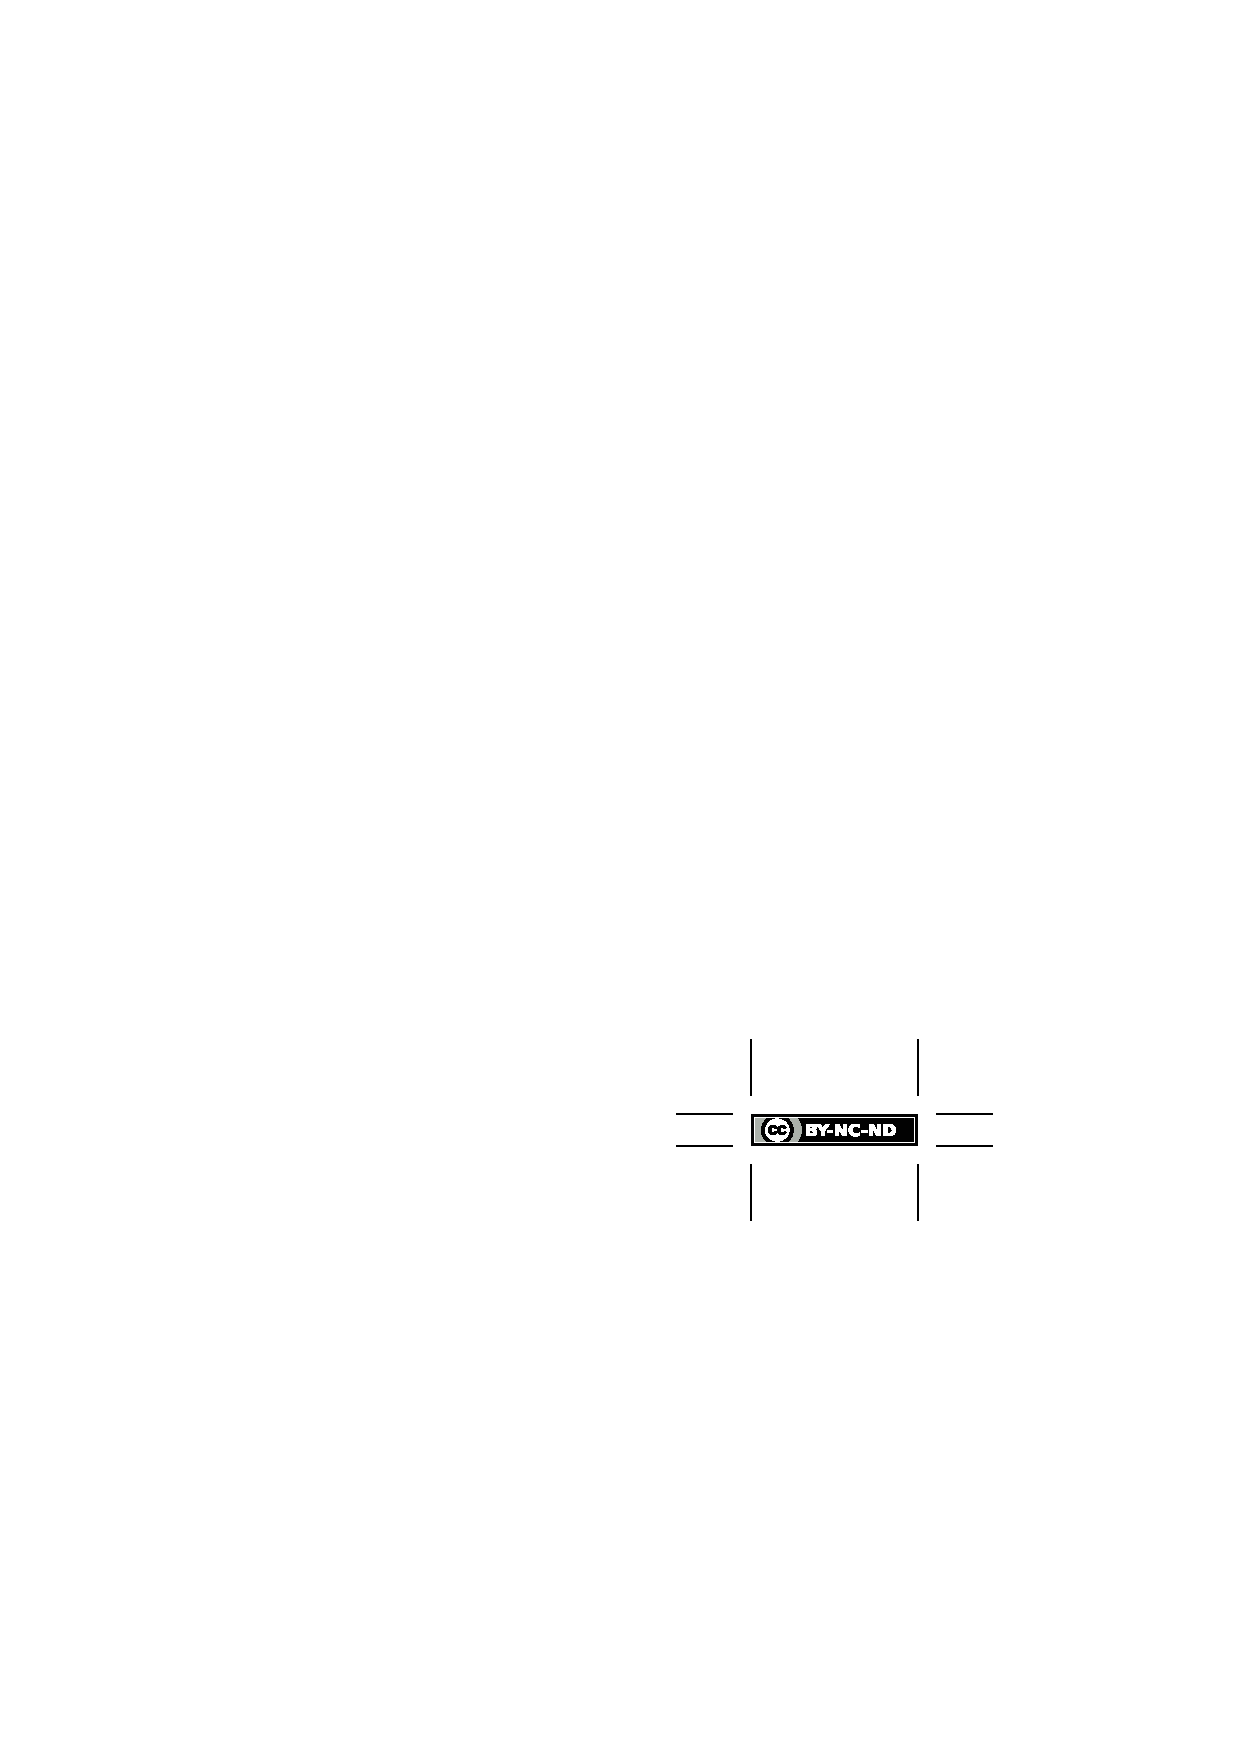
\includegraphics[height=11bp,clip]{by-nc-nd}\break
         \iflanguage{ngerman}
           {Dieses Werk ist lizenziert unter der Creative Commons Attribution-Non-\break
            Commercial-NoDerivatives 4.0 International Lizenz. Weitere Informationen\break
            finden Sie unter\space}%
           {This work is licensed under the Creative Commons Attribution-\break
            NonCommercial-NoDerivatives 4.0 License. For details go to\break}%
         \url{http://creativecommons.org/licenses/by-nc-nd/4.0/}.
         \vskip\baselineskip
       \fi
       \textbf{Library of Congress Cataloging-in-Publication Data}\\
       A CIP catalog record for this book has been applied 
         for at the Library of Congress.\par
       \vskip\baselineskip
       \iflanguage{ngerman}
        {\textbf{Bibliografische Information der Deutschen Nationalbibliothek}\\
         Die Deutsche Nationalbibliothek verzeichnet diese Publikation in der
         Deutschen Nationalbibliografie; detaillierte bibliografische Daten sind
         im Internet \"uber\break \url{http://dnb.dnb.de} abrufbar.}
        {\textbf{Bibliographic information published by the Deutsche Nationalbibliothek}\\
         The Deutsche Nationalbibliothek lists this publication in the
         Deutsche Nationalbibliografie;\\ detailed bibliographic data are 
         available on the Internet at \url{http://dnb.dnb.de}.}%
       \par\vskip\baselineskip
       \ifx\f@rmat b\relax\columnbreak\fi
       \textcopyright\space\@copyrightyear
       \ifx\@copyrighttext\@undefined
       \else
         \space\@copyrighttext,%
       \fi
       \ifx\@openaccess\relax\space\iflanguage{ngerman}{publiziert von}{published by}\fi%Claudia.Braeuer@degruyter.com
       \space Walter de Gruyter GmbH, Berlin/Boston
       \newline
       \ifx\@openaccess\relax
         \iflanguage{ngerman}
           {Dieses Buch ist als Open-Access-Publikation verfügbar über www.degruyter.com.}
           {The book is published with open access at www.degruyter.com.}
         \\[\baselineskip]
       \fi
       \ifx\@cover\@undefined\else
         \iflanguage{ngerman}{Umschlaggestaltung}{Cover image}:\space\@cover\\
       \fi
       \ifx\@typesetter\@undefined\else
         \iflanguage{ngerman}{Satz}{Typesetting}:\space\@typesetter\\
       \fi
       \ifx\@printbind\@undefined\else
         \iflanguage{ngerman}{Druck und Bindung}{Printing and binding}:\space\@printbind\\
       \fi
       \ifx\dgf@nts\relax
         \ifx\f@encoding\UTFencname\char"267E\else{\fontencoding{TS1}\selectfont\char"C9}\fi
       \else
         \textcircled{\raise0.4ex\hbox{\fontsize{4}{4}\selectfont$\infty$}}%
       \fi
       \space
       \iflanguage{ngerman}
         {Gedruckt auf s\"aurefreiem Papier}
         {Printed on acid-free paper}%
       \\
       Printed in Germany\par
       \vskip\baselineskip
       \url{www.degruyter.com}\par
       \ifx\f@rmat b\relax\end{multicols}\fi
     \egroup
     \if@tempswa\twocolumn\else\break\fi}}
%    \end{macrocode}
%
% Headings:
%    \begin{macrocode}
\setcounter{secnumdepth}{4}
\def\thefrontmatterpage{\csname @Roman\endcsname\c@page}
\@ifclassloaded{article}
 {}
 {\def\frontmatter{\cleardoublepage\@mainmatterfalse\pagenumbering{Roman}}
  \def\backmatter{\cleardoublepage\@mainmatterfalse\ifx\@margincolreset\@undefined\else\@margincolreset\fi}}
 
\@ifclassloaded{article}
 {\renewcommand\part{%
    \if@noskipsec\leavevmode\fi
    \par
    \addvspace{2\baselineskip}%
    \@afterindentfalse
    \secdef\@part\@spart}
  \def\@part[#1]#2{%
    \ifnum\c@secnumdepth>\m@ne
      \refstepcounter{part}%
      \addcontentsline{toc}{part}{\thepart\space#1}%
    \else
      \addcontentsline{toc}{part}{#1}%
    \fi
    {\parindent\z@\raggedright
     \interlinepenalty\@M
     \sffamily\Large
     \ifnum\c@secnumdepth>\m@ne
       \partname\nobreakspace\thepart
       \if!#2!\@empty\else:\space\fi
       \par\nobreak
     \fi
     \if!#2!\@empty\else\bfseries#2\fi
     \par}%
    \nobreak
    \vskip13\p@
    \@afterheading}
  \def\@spart#1{%
    {\parindent\z@\raggedright
     \interlinepenalty\@M
     \sffamily\Large
     \bfseries#1\par}%
    \nobreak
    \vskip13\p@
    \@afterheading}}
 {\let\@partmotto\@empty
  \def\partmotto#1{%
    \def\@partmotto{\vskip\dimexpr\baselineskip+2\p@\relax
                    \quote#1\endquote\global\let\@partmotto\@empty}}%
  \renewcommand\part{%
   \cleardoublepage
   \global\let\firstCh@fPart\relax
   \secdef\@part\@spart}
  \def\@part[#1]#2{%
    \ifnum\c@secnumdepth>-2\relax
      \refstepcounter{part}%
      \addcontentsline{toc}{part}{\protect\partnumberline{\mdseries\partname\ \thepart:\enskip}#1}%
    \else
      \addcontentsline{toc}{part}{#1}%
    \fi
    \markboth{\partname\ \thepart\enskip#1}{\partname\ \thepart\enskip#1}%
    \dg@barpage
      {}
      {\parindent\z@\raggedright
       \interlinepenalty\@M
       {\sffamily\Large
        \ifnum\c@secnumdepth>-2\relax
          \setbox\z@\hbox{%
            \partname\nobreakspace\thepart
            \if!#2!\@empty\else:\space\fi}%
          \hangindent\wd\z@
          \unhbox\z@
        \fi
        \if!#2!\@empty\else\bfseries#2\fi\par}%
        \@partmotto}}
  \def\@spart#1{%
    \dg@barpage
      {}
      {\parindent\z@\raggedright
       \interlinepenalty\@M
       {\sffamily\Large
        \bfseries#1\par}%
       \@partmotto}}}
\@ifclassloaded{article}
  {\relax}
  {\g@addto@macro\frontmatter{\global\let\componentd@i\z@}%
   \g@addto@macro\mainmatter{\global\let\componentd@i\z@}%
   \renewcommand\chapter{%
     \if@openright
       \cleardoublepage
     \else
       \ifx\firstCh@fPart\@undefined
         \clearpage
       \else
         \global\let\firstCh@fPart\@undefined
         \cleardoublepage
       \fi
     \fi
     \thispagestyle{plain}%
     \global\@topnum\z@
     \@afterindentfalse
     \secdef\@chapter\@schapter}
   \def\@chapter[#1]#2{%
     \let\thesection\theinchapsection
     \let\theequation\theinchapequation
     \let\thefigure\theinchapfigure
     \let\thetable\theinchaptable
     \ifx\bookDOI\@undefined
     \else
       \@tempcnta\numexpr\componentd@i+\@ne\relax
       \xdef\componentd@i{\the\@tempcnta}%
       \xdef\@DOI{%
         https://doi.org/\bookDOI
         -\ifx\thepage\thefrontmatterpage2\else\ifnum\@tempcnta<100 0\fi\fi
         \ifnum\@tempcnta<10 0\fi\componentd@i}%
     \fi
     \ifnum \c@secnumdepth >\m@ne
       \if@mainmatter
         \refstepcounter{chapter}%
         \typeout{\@chapapp\space\thechapter.}%
         \addcontentsline{toc}{chapter}{\protect\numberline{\thechapter}#1}%
       \else
         \addcontentsline{toc}{schapter}{#1}%
       \fi
     \else
       \addcontentsline{toc}{schapter}{#1}%
     \fi
     \chaptermark{#1}%
     \addtocontents{lof}{\protect\addvspace{13\p@}}%
     \addtocontents{lot}{\protect\addvspace{13\p@}}%
     \if@twocolumn
       \@topnewpage[\@makechapterhead{#2}]%
     \else
       \@makechapterhead{#2}%
       \@afterheading
     \fi}
   \def\@makechapterhead#1{%
     {\parindent\z@
      \raggedright
      \leavevmode
      \vrule\@width\z@\@height\dimexpr\topskip+0.5\baselineskip\relax\@depth\z@
      \sffamily\mathversion{ssbold}\bfseries
      \Large%should better be \LARGE
      \settowidth\hangindent{\thechapter\enskip}%
      \interlinepenalty\@M
      \ifnum \c@secnumdepth >\m@ne
        \if@mainmatter
          \thechapter\enskip
        \fi
      \fi
      #1\par\nobreak
      \vskip13\p@}%
     \ifx\@chapsubtitle\@undefined
     \else
       \@chapsubtitle\global\let\@chapsubtitle\@undefined
     \fi}
   \def\@schapter#1{%
     \setcounter{section}{\z@}%
     %%\let\thesection\theplainsection %remove 'cause as switch does harm 
     \let\theequation\theplainequation
     \let\thefigure\theplainfigure
     \let\thetable\theplaintable
     \ifx\bookDOI\@undefined
     \else
       \@tempcnta\numexpr\componentd@i+\@ne\relax
       \xdef\componentd@i{\the\@tempcnta}%
       \xdef\@DOI{%
         https://doi.org/\bookDOI
         -\ifx\thepage\thefrontmatterpage2\else0\fi
         \ifnum\@tempcnta<10 0\fi\componentd@i}%
     \fi
     \addcontentsline{toc}{schapter}{#1}%
     \chaptermark{#1}%
     \if@twocolumn
       \@topnewpage[\@makeschapterhead{#1}]%
     \else
       \@makeschapterhead{#1}%
       \@afterheading
     \fi}
   \def\@makeschapterhead#1{%
     {\parindent\z@
      \raggedright
      \leavevmode
      \vrule\@width\z@\@height\dimexpr\topskip+0.5\baselineskip\relax\@depth\z@
      \sffamily\mathversion{ssbold}\bfseries
      \Large%should better be \LARGE
      \interlinepenalty\@M
      #1\par\nobreak
      \vskip13\p@}}
   \let\theinchapsection\thesection
   \def\theplainsection{\arabic{section}}
   \let\theinchapequation\theequation
   \def\theplainequation{\arabic{equation}}
   \let\theinchapfigure\thefigure
   \def\theplainfigure{\arabic{figure}}
   \let\theinchaptable\thetable
   \def\theplaintable{\arabic{table}}}
\renewcommand\section{%
  \suppressfloats[t]%
  \@startsection{section}{1}{\z@}%
    {\ifx\thesection\theinchapsection-24\p@\else-26\p@\fi}%
    {13\p@}%
    {\raggedright\sffamily\bfseries\mathversion{ssbold}%
     \ifx\thesection\theinchapsection
       \large
     \else
       \Large\leavevmode\vrule\@width\z@\@height\dimexpr\topskip+6.5\p@\relax\@depth\z@
     \fi}}
\renewcommand\subsection{%
  \@startsection{subsection}{2}{\z@}%
    {\ifx\thesection\theinchapsection-26\p@\else-24\p@\fi}%
    {13\p@\@plus\z@\@minus4\p@}%
    {\raggedright\sffamily\bfseries\mathversion{ssbold}%
     \ifx\thesection\theinchapsection
       \normalsize
     \else
       \large
     \fi}}
\renewcommand\subsubsection{%
  \@startsection{subsubsection}{3}{\z@}%
    {\ifx\thesection\theinchapsection-19.5\p@\else-26\p@\fi}%
    {\ifx\thesection\theinchapsection1sp\else13\p@\fi}%
    {\raggedright\sffamily \normalsize\bfseries\mathversion{ssbold}}}
\renewcommand\paragraph{%
  \@startsection{paragraph}{4}{\z@}%
    {-19.5\p@}%
    {1sp}%
    {\raggedright\sffamily\normalsize\bfseries\mathversion{ssbold}}}
\renewcommand\subparagraph{%
  \@startsection{subparagraph}{5}{\z@}%
    {-19.5\p@}%
    {1sp}%
    {\raggedright\sffamily\normalsize\bfseries\mathversion{ssbold}}}
%    \end{macrocode}
%
% Lists: 
%    \begin{macrocode}
\leftmargini\parindent
\leftmargin\leftmargini
\leftmarginii\leftmargini
\leftmarginiii\leftmargini
\leftmarginiv\leftmargini
\leftmarginv\leftmargini
\def\labelitemi{\normalfont\textendash}
\def\labelitemii{\normalfont\textendash}
\renewenvironment{description}
 {\list{}{\topsep\z@
          \labelwidth\z@ \itemindent-\leftmargin
          \let\makelabel\descriptionlabel}}
 {\ifnum\@listdepth=\@ne\advance\@topsepadd\baselineskip\fi
  \endlist
  \gdef\@doendpe{%
    \@endpetrue
    \everypar{{\setbox\z@\lastbox}\everypar{}\@endpefalse}%
    \global\let\@doendpe\orig@doendpe}}
%    \end{macrocode}
%
% Quotes, quotations, and legal texts: 
%    \begin{macrocode}
\renewenvironment{quotation}
 {\list{}{\listparindent\parindent
          \itemindent   \listparindent
          \parsep       \z@}%
          \small
          \item\relax}
 {\endlist
  \gdef\@doendpe{%
    \@endpetrue
    \everypar{{\setbox\z@\lastbox}\everypar{}\@endpefalse}%
    \global\let\@doendpe\orig@doendpe}}
\renewenvironment{quote}
 {\list{}{}%
          \small
          \item\relax}
 {\endlist
  \gdef\@doendpe{%
    \@endpetrue
    \everypar{{\setbox\z@\lastbox}\everypar{}\@endpefalse}%
    \global\let\@doendpe\orig@doendpe}}
\newenvironment{legaltext}
 {\list{}{\topsep\baselineskip}%
          \bfseries
          \item
          \vrule\@height1.7\baselineskip\@width\z@}
 {\topsep\baselineskip
  \endlist}
%    \end{macrocode}
%
% Table of contents:
%    \begin{macrocode}
\renewcommand\tableofcontents{%
  \cleardoublepage
  \ifx\f@rmat b\else
    \if@twocolumn
      \@restonecoltrue\onecolumn
    \else
      \@restonecolfalse
    \fi
  \fi
  \thispagestyle{plain}%
  \@afterindentfalse
  \chaptermark{\contentsname}%
  \@makeschapterhead{\contentsname}%
  \let\lastentry@author\relax
  \@starttoc{toc}%
  \ifx\f@rmat b\else\if@restonecol\twocolumn\fi\fi}
\let\@issuetwocolcontentsline\@empty
\def\issuetableofcontents{%
  \global\c@tocdepth\z@
  \cleardoublepage
  \let\@mkboth\@gobbletwo
  \def\@pstring{%
    \ifx\@journalname\@undefined\else
      \@journalname
      \quad\dg@bartwo\quad
      \@journalyear
      \ifx\@journalvolume\@undefined\else
        \space|\space\volumename\space\@journalvolume
        \ifx\@journalissue\@undefined\else
          \space|\space\issuename\space\@journalissue
        \fi
      \fi
    \fi}
  \def\@oddhead{%
    \sffamily\small
    \usebox\dg@wordmark
    \hfil
    \@pstring}%
  \def\@evenhead{%
    \sffamily\small
    \@pstring
    \global\let\@DOI\@empty
    \hfil
    \usebox\dg@wordmark}%
  \let\@oddfoot\@empty
  \let\@evenfoot\@empty
  \ifx\f@rmat b%
    \setlength\dbltextfloatsep{49.5\p@ \@plus 2\p@ \@minus 4\p@}
    \twocolumn[%
      \vspace*{-26\p@}\section*{\contentsname}\vskip3\p@
      \ifx\@issuetwocolcontentsline\@empty\else
        \vskip3\p@%Maria.Dassing@degruyter.com 
        \sffamily\mathversion{ss}\@issuetwocolcontentsline\vskip24\p@
      \fi]%
    %\@nobreakfalse
  \else
    \section*{\contentsname}%
  \fi
  \let\lastentry@author\relax
  \@starttoc{toc}}
\def\l@part{\@dottedtocline{-1}{24\p@}{\bfseries\large}}
\def\l@chapter{\@dottedtocline{0}{13\p@}{}}
\def\l@schapter{\@dottedtocline{0}{13\p@}{\leftskip\z@}}
\def\l@section{\@dottedtocline{1}{\z@}{}}
\def\l@subsection{\@dottedtocline{2}{\z@}{}}
\def\l@subsubsection{\@dottedtocline{3}{\z@}{}}
\def\l@paragraph{\@dottedtocline{4}{\z@}{}}
\def\l@subparagraph{\@dottedtocline{5}{\z@}{}}
\def\l@author#1#2{\vskip13\p@{\raggedright#1\par}\let\lastentry@author\relax}
\def\l@tocsection#1#2{%only for issuetocs
  \if@nobreak\vspace*{-2\p@}\@nobreakfalse\if@twocolumn\else\vskip\baselineskip\fi\else\vskip24\p@\fi
  {\raggedright\large\bfseries#1\par}\vskip1sp}
\def\l@tocsubsection#1#2{%only for issuetocs
  \if@nobreak\vskip-\tw@\p@\@nobreakfalse\else\ifdim\lastskip>\z@\vskip6\p@\else\vskip24\p@\fi\fi % 6 statt 13 %Maria.Dassing@degruyter.com
  {\raggedright\large\mdseries#1\par}}
\def\addissuecontentsline#1#2{\@writefile{toc}{\contentsline{#1}{#2}{}{}}}%only for issuetocs
\def\addissuetwocolcontentsline#1#2{%
  \protected@write\@auxout{}{\string\g@addto@macro\string\@issuetwocolcontentsline{\string\contentsline{#1}{#2}{}{}}}}%only for issuetocs
\renewcommand\listoffigures{%
  \if@twocolumn
    \@restonecoltrue\onecolumn
  \else
    \@restonecolfalse
  \fi
  \chapter*{\listfigurename}%
  {\small%Maria.Dassing@degruyter.com
   \@starttoc{lof}}%
  \if@restonecol\twocolumn\fi}
\def\l@figure{\@dottedtocline{1}{\z@}{}}
\renewcommand\listoftables{%
  \if@twocolumn
    \@restonecoltrue\onecolumn
  \else
    \@restonecolfalse
  \fi
  \chapter*{\listtablename}%
  {\small%Maria.Dassing@degruyter.com
   \@starttoc{lot}}%
  \if@restonecol\twocolumn\fi}
\def\l@table{\@dottedtocline{1}{\z@}{}}
%    \end{macrocode}
%
% Layout setting for the bibliography:
%    \begin{macrocode}
\bibindent\parindent
%    \end{macrocode}
%
% The |{index}| environment and related commands:
%    \begin{macrocode}
\let\indexpreamble\@empty
\renewenvironment{theindex}
 {\if@twocolumn
    \@restonecolfalse
  \else
    \@restonecoltrue
  \fi
  \sffamily\mathversion{ss}\small
  \begin{multicols}{2}%
    [\chapter*{\indexname}%
     \indexpreamble]
  \raggedright
  \parskip\z@ \@plus .3\p@\relax
  \columnseprule \z@
  \let\item\@idxitem}
 {\end{multicols}%
  \if@restonecol\onecolumn\fi
  \cleardoublepage}
\renewcommand\@idxitem{\par\let\idxlevel=\@ne\hangindent6mm}
\renewcommand\subitem{\par
  \ifx\idxlevel\@ne\let\idxlevel=\tw@\nopagebreak\fi
  \hangindent6mm\leavevmode\hb@xt@0.75em{\textendash\hss}}
\renewcommand\subsubitem{\par
  \ifx\idxlevel\tw@\let\idxlevel=\thr@@\nopagebreak\fi
  \hangindent6mm\leavevmode\hb@xt@1.5em{\kern0.75em\textendash\hss}}
\renewcommand\indexspace{\par\vskip11\p@\@plus5\p@\@minus3\p@\relax}
%    \end{macrocode}
%
% For footnotes see below. 
%
% Setting |\columnsep| to the grid sep:
%    \begin{macrocode}
\columnsep4mm
%    \end{macrocode}
%
% Always ``ragged'' pages:
%    \begin{macrocode}
\raggedbottom
%    \end{macrocode}
%
% \subsection{Providing and adapting packages}
%
% \subsubsection{Glyph mapping information}
%
%    \begin{macrocode}
\ifx\XeTeXcharclass\@undefined
  \ifx\directlua\undefined\ifnum\pdfoutput>\z@
    \IfFileExists{dummy-space.pfb}{\pdfinterwordspaceon}{}
    \RequirePackage{cmap}
  \fi\fi
  \InputIfFileExists{glyphtounicode.tex}{}{}
  \pdfgentounicode=1
\fi
%    \end{macrocode}
%
% \subsubsection{Fonts}
%
% Output encoding\\
% (note that the tipa package must be loaded before activating T1 and TS1 encodings):
%    \begin{macrocode}
\@ifpackageloaded{fontspec}
 {\ifx\IfFontExistsTF\@undefined
    \PackageError{dgruyter}
      {Version `2017/03/31' of package fontspec is required}%
      {Please update the fontspec package, or font support might be incomplete.\space}
    \let\IfFontExistsTF\@thirdofthree
  \fi
  \RequirePackage[intlimits,tbtags]{amsmath}
  \RequirePackage{unicode-math}[2015/07/29 v0.8]
  \ifx\symnormal\@undefined
    \PackageError{dgruyter}
      {Version `2015/07/29' of package unicode-math is required}%
      {Please update the unicode-math package, or math-font support won't work.\space}
  \fi}
 {\let\addfontfeature\@gobble
  \let\addfontfeatures\@gobble
  \let\old@sups\sups
  \let\sups\@undefined
  \RequirePackage[safe]{tipa}
  \let\sups\old@sups
  \RequirePackage[T1]{fontenc}}
\RequirePackage{textcomp}
%    \end{macrocode}
%
% New math versions required for DGMeta + MinionMath fonts:
%    \begin{macrocode}
\DeclareMathVersion{ss}
\DeclareMathVersion{ssbold}
%    \end{macrocode}
%
% The typewriter font:
%    \begin{macrocode}
\@ifpackageloaded{fontspec}
 {\IfFontExistsTF{Inconsolatazi4-Regular.otf}
   {\setmonofont[StylisticSet=3,%Maria.Dassing@degruyter.com
                 BoldFont  =Inconsolatazi4-Bold.otf]
                           {Inconsolatazi4-Regular.otf}
    \setmathfontface\mathtt{Inconsolatazi4-Regular.otf}
    \setmathfontface\mathtt{Inconsolatazi4-Bold.otf}[version=bold]
    \setmathfontface\mathtt{Inconsolatazi4-Bold.otf}[version=ssbold]}
   {\setmonofont[ItalicFont=lmmonolt10-oblique.otf,
           BoldFont        =lmmonolt10-bold.otf,
           BoldItalicFont  =lmmonolt10-boldoblique.otf]
                           {lmmonolt10-regular.otf}
    \setmathfontface\mathtt{lmmonolt10-regular.otf}
    \setmathfontface\mathtt{lmmonolt10-bold.otf}[version=bold]
    \setmathfontface\mathtt{lmmonolt10-bold.otf}[version=ssbold]}}
 {\IfFileExists{zi4.sty}
   {\RequirePackage{zi4}}
   {\def\ttdefault{lmtt}\let\lmtt@use@light@as@normal\@empty}}
%    \end{macrocode}
% 
% If the DG\,Meta fonts are installed they will be used, otherwise Latin~Modern will be used as
% fallback:
%    \begin{macrocode}
\ifx\f@encoding\UTFencname
  \IfFontExistsTF{DGMetaSerifScience-Regular.otf}{\let\dgf@nts\relax}{}
\else
  \IfFileExists{DGMetaSerifScience.sty}{\let\dgf@nts\relax}{}
\fi
%    \end{macrocode}
%
% First, the fallback case with Latin~Modern:
%    \begin{macrocode}
\ifx\dgf@nts\@undefined
  \@ifpackageloaded{unicode-math}{}{\RequirePackage{amssymb}}
%    \end{macrocode}
% 
% Now, the case with the DG\,Meta fonts (with math alphabets and symbols possibly from MinionMath):\\
% -- additions for the fontspec font mode:
%    \begin{macrocode}
\else
  \@ifpackageloaded{fontspec}
   {\ifx\bfseries@rm\@undefined\else\let\bfdefault\bfseries@rm\fi%avoid mweights--fontspec trouble
    \setmainfont[ItalicFont    =DGMetaSerifScience-Italic.otf,
                 BoldFont      =DGMetaSerifScience-Bold.otf,
                 BoldItalicFont=DGMetaSerifScience-BoldItalic.otf]
                               {DGMetaSerifScience-Regular.otf}
    \setsansfont[ItalicFont    =DGMetaScience-Italic.otf,
                 BoldFont      =DGMetaScience-Bold.otf,
                 BoldItalicFont=DGMetaScience-BoldItalic.otf]
                               {DGMetaScience-Regular.otf}
    \RequirePackage{realscripts}
    \IfFontExistsTF{MinionMath-Medium.otf}
     {%from typoma GmbH:
      \setmathfont{MinionMath-Medium.otf}%
        [SizeFeatures  = {
          {Size = -6   , RawFeature = {+ssty=1}, Font = MinionMath-MediumTiny.otf},
          {Size = 6-8.4, RawFeature = {+ssty=1}, Font = MinionMath-MediumCapt.otf},
          {Size = 8.4- , RawFeature = {+ssty=1}, Font = MinionMath-Medium.otf}}]
      \setmathfont{MinionMath-Bold.otf}[range={bfup->up,bfit->it}]
      \setmathfont{MinionMath-Bold.otf}[version=bold]
      \setmathfont{MinionMath-Medium.otf}[version=ss]
      \setmathfont{MinionMath-Bold.otf}[version=ssbold]}
     {\setmathfont{latinmodern-math.otf}
      \setmathfont{latinmodern-math.otf}[version=ss]
      \setmathfont{latinmodern-math.otf}[version=ssbold]}
    %\setmathfont{DGMetaSerifScience-Italic.otf}[range=it/{latin,Latin,num,Greek,greek},LetterSpace=5.5]
    %\setmathfont{DGMetaSerifScience-BoldItalic.otf}[version=bold,range=it/{latin,Latin,num,Greek,greek},LetterSpace=5.5] % -- geht nicht
    %\setmathfont{DGMetaScience-Italic.otf}[version=ss,range=it/{latin,Latin,num,Greek,greek},LetterSpace=5.5] % -- geht nicht
    %\setmathfont{DGMetaScience-BoldItalic.otf}[version=ssbold,range=it/{latin,Latin,num,Greek,greek},LetterSpace=5.5] % -- geht nicht
    %\setmathfontface\mathrm{DGMetaSerifScience-Regular.otf}
    %\setmathfontface\mathrm{DGMetaSerifScience-Bold.otf}[version=bold]
    %\setmathfontface\mathrm{DGMetaScience-Regular.otf}[version=ss]%mind
    %\setmathfontface\mathrm{DGMetaScience-Bold.otf}[version=ssbold]%mind
    %\setmathfontface\mathit{DGMetaSerifScience-Italic.otf}
    %\setmathfontface\mathit{DGMetaSerifScience-BoldItalic.otf}[version=bold]
    %\setmathfontface\mathit{DGMetaScience-Italic.otf}[version=ss]%mind
    %\setmathfontface\mathit{DGMetaScience-BoldItalic.otf}[version=ssbold]%mind
    %\setmathfontface\mathbf{DGMetaSerifScience-Bold.otf}
    %\setmathfontface\mathbf{DGMetaScience-Bold.otf}[version=ss]%mind
    %\setmathfontface\mathbf{DGMetaScience-Bold.otf}[version=ssbold]%mind
    %\setmathfontface\mathsf{DGMetaScience-Regular.otf}
    %\setmathfontface\mathsf{DGMetaScience-Bold.otf}[version=bold]
    %\setmathfontface\mathsf{DGMetaScience-Bold.otf}[version=ssbold]
    \let\mathfrak\@undefined
    \RequirePackage{eucal,eufrak,mathrsfs}
    \SetMathAlphabet\EuScript{ssbold}{U}{eus}{b}{n}
    \SetMathAlphabet\EuFrak{ssbold}{U}{euf}{b}{n}
    \IfFontExistsTF{Inconsolatazi4-Regular.otf}
     {\setmathfontface\mathtt{Inconsolatazi4-Regular.otf}
      \setmathfontface\mathtt{Inconsolatazi4-Bold.otf}[version=bold]
      \setmathfontface\mathtt{Inconsolatazi4-Bold.otf}[version=ssbold]}
     {\setmathfontface\mathtt{lmmonolt10-regular.otf}
      \setmathfontface\mathtt{lmmonolt10-bold.otf}[version=bold]
      \setmathfontface\mathtt{lmmonolt10-bold.otf}[version=ssbold]}}
%    \end{macrocode}
% -- additions for the classical nfss font mode:
%    \begin{macrocode}
   {\usepackage[lining,proportional]{DGMetaScience}
    \usepackage[lining,proportional]{DGMetaSerifScience}
    \def\thestandardf@@tnote{\@arabic\c@footnote}
    \def\@makefnmark{%
      \hbox{%
        \ifx\thefootnote\thestandardf@@tnote
          \expandafter\ifx\thempfn\thempfootnote
            \@textsuperscript{\selectfont\thempfn}%
          \else
            \fontencoding{U}\upshape\@thefnmark
          \fi
        \else
          \@textsuperscript{\upshape\@thefnmark}%
        \fi}}
    \IfFileExists{minionmath.sty}
      {\IfFileExists{mmathdgm.sty}
         {\RequirePackage[withamsmath,amssymb,extraops]{mmathdgm}}
         {\RequirePackage[withamsmath,amssymb,extraops]{minionmath}
          \SetMathAlphabet{\mathrm}    {bold}  {T1} {minionmath}{b}{n} %mind! (gives more flexibility)
          \SetMathAlphabet{\mathrm}    {ss}    {T1} {cmss}      {m}{n} %mind! (gives more flexibility)
          \SetMathAlphabet{\mathrm}    {ssbold}{T1} {cmss}      {bx}{n} %mind! (gives more flexibility)
          \SetSymbolFont{operators}    {ssbold}{T1} {minionmath}{b} {n}
          \SetSymbolFont{letters}      {ssbold}{MSP}{minionmath-rsfs}{b} {n}
          \SetSymbolFont{symbols}      {ssbold}{MC} {minionmath}{b} {n}
          \SetMathAlphabet{\mathit}    {ssbold}{T1} {minionmath}{b} {it}
          \SetMathAlphabet{\mathsf}    {ssbold}{T1} {cmss}      {bx}{n}
          \SetSymbolFont{largesymbols} {ssbold}{MXP}{minionmath}{b} {\@extshape}
          \DeclareMathAlphabet{\mathit}  {T1}{MinionPro-TLF}{m}{it}%patch (because resp. minionmath font not provided)
          \SetMathAlphabet{\mathit}{bold}{T1}{MinionPro-TLF}{b}{it}%patch (because resp. minionmath font not provided)
          \DeclareMathAlphabet{\mathbold}{T1}{MinionPro-TLF}{b}{it}%patch (because resp. minionmath font not provided)
          \SetMathAlphabet{\mathbold}{ss}{T1}{cmss}{bx}{it}%
          \SetMathAlphabet{\mathbold}{ssbold}{T1}{cmss}{bx}{it}%
          \DeclareMathSizes{8}{8.8}{\@viipt}{\@vpt}%"scale" minionmath-Fonts to 110%
          \DeclareMathSizes{9.5}{10.5}{\@viipt}{\@vpt}%"scale" minionmath-Fonts to 110%
          \DeclareMathSizes{15}{16.5}{\@xpt}{\@viiipt}%"scale" minionmath-Fonts to 110%
          \DeclareMathSizes{22}{24.2}{15}{13}%"scale" minionmath-Fonts to 110%
          \DeclareMathSizes{24}{26.4}{\@xxpt}{\@xviipt}}%"scale" minionmath-Fonts to 110%
      \SetSymbolFont{symbolsb}     {ssbold}{MS1}{minionmath}{b}{n}
      \SetSymbolFont{symbolsc}     {ssbold}{MS2}{minionmath-eufr}{b}{n}
      \@ifisencoding{MX1}{\SetSymbolFont{largesymbolsb}{ssbold}{MX1}{minionmath}{b}{\@extshape}}{}
      \DeclareMathSymbol{\triangle}{\mathord}{letters}{"86}%patch
      \global\let\restriction\upharpoonright%patch (cf. amssymb.sty) 
      \DeclareSymbolFontAlphabet{\mathscr}{letters}
      \RequirePackage{eucal}
      \SetMathAlphabet\EuScript{ssbold}{U}{eus}{b}{n}
      \let\Alpha\Alphait
      \let\Beta\Betait
      \let\Gamma\Gammait
      \let\Delta\Deltait
      \let\Epsilon\Epsilonit
      \let\Zeta\Zetait
      \let\Eta\Etait
      \let\Theta\Thetait
      \let\Iota\Iotait
      \let\Kappa\Kappait
      \let\Lambda\Lambdait
      \let\Mu\Muit
      \let\Nu\Nuit
      \let\Xi\Xiit
      \let\Omicron\Omicronit
      \let\Pi\Piit
      \let\Rho\Rhoit
      \let\Sigma\Sigmait
      \let\Tau\Tauit
      \let\Upsilon\Upsilonit
      \let\Phi\Phiit
      \let\Chi\Chiit
      \let\Psi\Psiit
      \let\Omega\Omegait
      \let\varUpsilon\varUpsilonit
      \let\varChi\varChiit
      \let\upAlpha\Alphaup
      \let\upBeta\Betaup
      \let\upGamma\Gammaup
      \let\upDelta\Deltaup
      \let\upEpsilon\Epsilonup
      \let\upZeta\Zetaup
      \let\upEta\Etaup
      \let\upTheta\Thetaup
      \let\upIota\Iotaup
      \let\upKappa\Kappaup
      \let\upLambda\Lambdaup
      \let\upMu\Muup
      \let\upNu\Nuup
      \let\upXi\Xiup
      \let\upOmicron\Omicronup
      \let\upPi\Piup
      \let\upRho\Rhoup
      \let\upSigma\Sigmaup
      \let\upTau\Tauup
      \let\upUpsilon\Upsilonup
      \let\upPhi\Phiup
      \let\upChi\Chiup
      \let\upPsi\Psiup
      \let\upOmega\Omegaup
      \let\upvarUpsilon\varUpsilonup
      \let\upvarChi\varChiup
      \let\upalpha\alphaup
      \let\upbeta\betaup
      \let\upgamma\gammaup
      \let\updelta\deltaup
      \let\upepsilon\epsilonup
      \let\upzeta\zetaup
      \let\upeta\etaup
      \let\uptheta\thetaup
      \let\upiota\iotaup
      \let\upkappa\kappaup
      \let\uplambda\lambdaup
      \let\upmu\muup
      \let\upnu\nuup
      \let\upxi\xiup
      \let\upomicron\omicronup
      \let\uppi\piup
      \let\uprho\rhoup
      \let\upsigma\sigmaup
      \let\uptau\tauup
      \let\upupsilon\upsilonup
      \let\upphi\phiup
      \let\upchi\chiup
      \let\uppsi\psiup
      \let\upomega\omegaup
      \let\upvarepsilon\varepsilonup
      \let\upvartheta\varthetaup
      \let\upvarkappa\varkappaup
      \let\upvarpi\varpiup
      \let\upvarrho\varrhoup
      \let\upvarsigma\varsigmaup
      \let\upvarphi\varphiup}
     {\RequirePackage{amssymb}
      \DeclareSymbolFont{operators}          {OT1}{DGMetaSerifScience-TLF}{m}{n}
      \DeclareSymbolFont{dgmetaletters}      {OML}{DGMetaSerifScience-TLF}{m}{it}
      \DeclareSymbolFont{dgmetalettersup}    {OML}{DGMetaSerifScience-TLF}{m}{n}
      \DeclareSymbolFont{dgmetasymbols}      {OMS}{DGMetaSerifScience-TLF}{m}{n}
      \DeclareMathAlphabet\mathbf            {OT1}{DGMetaSerifScience-TLF}{b}{n}
      \DeclareMathAlphabet\mathsf            {OT1}{DGMetaScience-TLF}     {m}{n}
      \DeclareMathAlphabet\mathit            {OT1}{DGMetaSerifScience-TLF}{m}{it}
      \DeclareMathAlphabet\mathtt            {OT1}{\ttdefault}            {m}{n}
      \SetSymbolFont{dgmetaletters}  {bold}  {OML}{DGMetaSerifScience-TLF}{b}{it}
      \SetSymbolFont{dgmetalettersup}{bold}  {OML}{DGMetaSerifScience-TLF}{b}{n}
      \SetSymbolFont{dgmetasymbols}  {bold}  {OMS}{DGMetaSerifScience-TLF}{b}{n}
      \SetSymbolFont{operators}      {bold}  {OT1}{DGMetaSerifScience-TLF}{b}{n}
      \SetMathAlphabet\mathsf        {bold}  {OT1}{DGMetaScience-TLF}     {b}{n}
      \SetMathAlphabet\mathit        {bold}  {OT1}{DGMetaSerifScience-TLF}{b}{it}
      \SetSymbolFont{operators}      {ss}    {OT1}{\sfdefault}            {m}{n}
      \SetSymbolFont{letters}        {ss}    {OML}{cmss}                  {m}{it}
      \SetSymbolFont{dgmetaletters}  {ss}    {OML}{DGMetaScience-TLF}     {m}{it}
      \SetSymbolFont{dgmetalettersup}{ss}    {OML}{DGMetaScience-TLF}     {m}{n}
      \SetSymbolFont{dgmetasymbols}  {ss}    {OMS}{DGMetaScience-TLF}     {m}{n}
      \SetMathAlphabet\mathit        {ss}    {OT1}{\sfdefault}            {m}{it}
      \SetMathAlphabet\mathbf        {ss}    {OT1}{\sfdefault}            {b}{n}
      \SetMathAlphabet\mathtt        {ss}    {OT1}{\ttdefault}            {m}{n}
      \SetSymbolFont{operators}      {ssbold}{OT1}{\sfdefault}            {b}{n}
      \SetSymbolFont{letters}        {ssbold}{OML}{cmss}                  {b}{it}
      \SetSymbolFont{symbols}        {ssbold}{OMS}{cmss}                  {b}{n}
      \SetSymbolFont{dgmetaletters}  {ssbold}{OML}{DGMetaScience-TLF}     {b}{it}
      \SetSymbolFont{dgmetalettersup}{ssbold}{OML}{DGMetaScience-TLF}     {b}{n}
      \SetSymbolFont{dgmetasymbols}  {ssbold}{OMS}{DGMetaScience-TLF}     {b}{n}
      \SetMathAlphabet\mathit        {ssbold}{OT1}{\sfdefault}            {b}{it}
      \SetMathAlphabet\mathbf        {ssbold}{OT1}{\sfdefault}            {b}{n}
      \SetMathAlphabet\mathsf        {ssbold}{OT1}{\sfdefault}            {b}{n}
      \SetMathAlphabet\mathtt        {ssbold}{OT1}{\ttdefault}            {b}{n}
      \DeclareMathSymbol{a}{\mathalpha}{dgmetaletters}{`a}
      \DeclareMathSymbol{b}{\mathalpha}{dgmetaletters}{`b}
      \DeclareMathSymbol{c}{\mathalpha}{dgmetaletters}{`c}
      \DeclareMathSymbol{d}{\mathalpha}{dgmetaletters}{`d}
      \DeclareMathSymbol{e}{\mathalpha}{dgmetaletters}{`e}
      \DeclareMathSymbol{f}{\mathalpha}{dgmetaletters}{`f}
      \DeclareMathSymbol{g}{\mathalpha}{dgmetaletters}{`g}
      \DeclareMathSymbol{h}{\mathalpha}{dgmetaletters}{`h}
      \DeclareMathSymbol{i}{\mathalpha}{dgmetaletters}{`i}
      \DeclareMathSymbol{j}{\mathalpha}{dgmetaletters}{`j}
      \DeclareMathSymbol{k}{\mathalpha}{dgmetaletters}{`k}
      \DeclareMathSymbol{l}{\mathalpha}{dgmetaletters}{`l}
      \DeclareMathSymbol{m}{\mathalpha}{dgmetaletters}{`m}
      \DeclareMathSymbol{n}{\mathalpha}{dgmetaletters}{`n}
      \DeclareMathSymbol{o}{\mathalpha}{dgmetaletters}{`o}
      \DeclareMathSymbol{p}{\mathalpha}{dgmetaletters}{`p}
      \DeclareMathSymbol{q}{\mathalpha}{dgmetaletters}{`q}
      \DeclareMathSymbol{r}{\mathalpha}{dgmetaletters}{`r}
      \DeclareMathSymbol{s}{\mathalpha}{dgmetaletters}{`s}
      \DeclareMathSymbol{t}{\mathalpha}{dgmetaletters}{`t}
      \DeclareMathSymbol{u}{\mathalpha}{dgmetaletters}{`u}
      \DeclareMathSymbol{v}{\mathalpha}{dgmetaletters}{`v}
      \DeclareMathSymbol{w}{\mathalpha}{dgmetaletters}{`w}
      \DeclareMathSymbol{x}{\mathalpha}{dgmetaletters}{`x}
      \DeclareMathSymbol{y}{\mathalpha}{dgmetaletters}{`y}
      \DeclareMathSymbol{z}{\mathalpha}{dgmetaletters}{`z}
      \DeclareMathSymbol{A}{\mathalpha}{dgmetaletters}{`A}
      \DeclareMathSymbol{B}{\mathalpha}{dgmetaletters}{`B}
      \DeclareMathSymbol{C}{\mathalpha}{dgmetaletters}{`C}
      \DeclareMathSymbol{D}{\mathalpha}{dgmetaletters}{`D}
      \DeclareMathSymbol{E}{\mathalpha}{dgmetaletters}{`E}
      \DeclareMathSymbol{F}{\mathalpha}{dgmetaletters}{`F}
      \DeclareMathSymbol{G}{\mathalpha}{dgmetaletters}{`G}
      \DeclareMathSymbol{H}{\mathalpha}{dgmetaletters}{`H}
      \DeclareMathSymbol{I}{\mathalpha}{dgmetaletters}{`I}
      \DeclareMathSymbol{J}{\mathalpha}{dgmetaletters}{`J}
      \DeclareMathSymbol{K}{\mathalpha}{dgmetaletters}{`K}
      \DeclareMathSymbol{L}{\mathalpha}{dgmetaletters}{`L}
      \DeclareMathSymbol{M}{\mathalpha}{dgmetaletters}{`M}
      \DeclareMathSymbol{N}{\mathalpha}{dgmetaletters}{`N}
      \DeclareMathSymbol{O}{\mathalpha}{dgmetaletters}{`O}
      \DeclareMathSymbol{P}{\mathalpha}{dgmetaletters}{`P}
      \DeclareMathSymbol{Q}{\mathalpha}{dgmetaletters}{`Q}
      \DeclareMathSymbol{R}{\mathalpha}{dgmetaletters}{`R}
      \DeclareMathSymbol{S}{\mathalpha}{dgmetaletters}{`S}
      \DeclareMathSymbol{T}{\mathalpha}{dgmetaletters}{`T}
      \DeclareMathSymbol{U}{\mathalpha}{dgmetaletters}{`U}
      \DeclareMathSymbol{V}{\mathalpha}{dgmetaletters}{`V}
      \DeclareMathSymbol{W}{\mathalpha}{dgmetaletters}{`W}
      \DeclareMathSymbol{X}{\mathalpha}{dgmetaletters}{`X}
      \DeclareMathSymbol{Y}{\mathalpha}{dgmetaletters}{`Y}
      \DeclareMathSymbol{Z}{\mathalpha}{dgmetaletters}{`Z}
      \DeclareMathSymbol{,}{\mathpunct}{dgmetalettersup}{"3B}
      \DeclareMathSymbol{.}{\mathord}{dgmetalettersup}{"3A}
      \DeclareMathSymbol{<}{\mathrel}{dgmetalettersup}{"3C}
      \DeclareMathSymbol{>}{\mathrel}{dgmetalettersup}{"3E}
      \DeclareMathSymbol{/}{\mathord}{dgmetalettersup}{"3D}
      \DeclareMathSymbol{\imath}{\mathord}{dgmetaletters}{"7B}
      \DeclareMathSymbol{\jmath}{\mathord}{dgmetaletters}{"7C}
      \DeclareMathSymbol{\partial}{\mathord}{dgmetaletters}{"40}
      \DeclareMathSymbol{\ldotp}{\mathpunct}{dgmetaletters}{"3A}
      \DeclareMathSymbol{\Gamma}{\mathord}{dgmetaletters}{0}
      \DeclareMathSymbol{\Delta}{\mathord}{dgmetaletters}{1}
      \DeclareMathSymbol{\Theta}{\mathord}{dgmetaletters}{2}
      \DeclareMathSymbol{\Lambda}{\mathord}{dgmetaletters}{3}
      \DeclareMathSymbol{\Xi}{\mathord}{dgmetaletters}{4}
      \DeclareMathSymbol{\Pi}{\mathord}{dgmetaletters}{5}
      \DeclareMathSymbol{\Sigma}{\mathord}{dgmetaletters}{6}
      \DeclareMathSymbol{\Upsilon}{\mathord}{dgmetaletters}{7}
      \DeclareMathSymbol{\Phi}{\mathord}{dgmetaletters}{8}
      \DeclareMathSymbol{\Psi}{\mathord}{dgmetaletters}{9}
      \DeclareMathSymbol{\Omega}{\mathord}{dgmetaletters}{10}
      \DeclareMathSymbol{\alpha}{\mathord}{dgmetaletters}{"0B}               
      \DeclareMathSymbol{\beta}{\mathord}{dgmetaletters}{"0C}
      \DeclareMathSymbol{\gamma}{\mathord}{dgmetaletters}{"0D}
      \DeclareMathSymbol{\delta}{\mathord}{dgmetaletters}{"0E}
      \DeclareMathSymbol{\epsilon}{\mathord}{dgmetaletters}{"0F}
      \DeclareMathSymbol{\zeta}{\mathord}{dgmetaletters}{"10}
      \DeclareMathSymbol{\eta}{\mathord}{dgmetaletters}{"11}
      \DeclareMathSymbol{\theta}{\mathord}{dgmetaletters}{"12}
      \DeclareMathSymbol{\iota}{\mathord}{dgmetaletters}{"13}
      \DeclareMathSymbol{\kappa}{\mathord}{dgmetaletters}{"14}
      \DeclareMathSymbol{\lambda}{\mathord}{dgmetaletters}{"15}
      \DeclareMathSymbol{\mu}{\mathord}{dgmetaletters}{"16}
      \DeclareMathSymbol{\nu}{\mathord}{dgmetaletters}{"17}
      \DeclareMathSymbol{\xi}{\mathord}{dgmetaletters}{"18}
      \DeclareMathSymbol{\pi}{\mathord}{dgmetaletters}{"19}
      \DeclareMathSymbol{\rho}{\mathord}{dgmetaletters}{"1A}
      \DeclareMathSymbol{\sigma}{\mathord}{dgmetaletters}{"1B}
      \DeclareMathSymbol{\tau}{\mathord}{dgmetaletters}{"1C}
      \DeclareMathSymbol{\upsilon}{\mathord}{dgmetaletters}{"1D}
      \DeclareMathSymbol{\phi}{\mathord}{dgmetaletters}{"1E}
      \DeclareMathSymbol{\chi}{\mathord}{dgmetaletters}{"1F}
      \DeclareMathSymbol{\psi}{\mathord}{dgmetaletters}{"20}
      \DeclareMathSymbol{\omega}{\mathord}{dgmetaletters}{"21}
      \DeclareMathSymbol{\varepsilon}{\mathord}{dgmetaletters}{"22}
      \DeclareMathSymbol{\vartheta}{\mathord}{dgmetaletters}{"23}
      \DeclareMathSymbol{\varpi}{\mathord}{dgmetaletters}{"24}
      \DeclareMathSymbol{\varrho}{\mathord}{dgmetaletters}{"25}
      \DeclareMathSymbol{\varsigma}{\mathord}{dgmetaletters}{"26}
      \DeclareMathSymbol{\varphi}{\mathord}{dgmetaletters}{"27}
      \DeclareMathSymbol{\upGamma}{\mathord}{dgmetalettersup}{0}
      \DeclareMathSymbol{\upDelta}{\mathord}{dgmetalettersup}{1}
      \DeclareMathSymbol{\upTheta}{\mathord}{dgmetalettersup}{2}
      \DeclareMathSymbol{\upLambda}{\mathord}{dgmetalettersup}{3}
      \DeclareMathSymbol{\upXi}{\mathord}{dgmetalettersup}{4}
      \DeclareMathSymbol{\upPi}{\mathord}{dgmetalettersup}{5}
      \DeclareMathSymbol{\upSigma}{\mathord}{dgmetalettersup}{6}
      \DeclareMathSymbol{\upUpsilon}{\mathord}{dgmetalettersup}{7}
      \DeclareMathSymbol{\upPhi}{\mathord}{dgmetalettersup}{8}
      \DeclareMathSymbol{\upPsi}{\mathord}{dgmetalettersup}{9}
      \DeclareMathSymbol{\upOmega}{\mathord}{dgmetalettersup}{10}
      \DeclareMathSymbol{\upalpha}{\mathord}{dgmetalettersup}{"0B}
      \DeclareMathSymbol{\upbeta}{\mathord}{dgmetalettersup}{"0C}
      \DeclareMathSymbol{\upgamma}{\mathord}{dgmetalettersup}{"0D}
      \DeclareMathSymbol{\updelta}{\mathord}{dgmetalettersup}{"0E}
      \DeclareMathSymbol{\upepsilon}{\mathord}{dgmetalettersup}{"0F}
      \DeclareMathSymbol{\upzeta}{\mathord}{dgmetalettersup}{"10}
      \DeclareMathSymbol{\upeta}{\mathord}{dgmetalettersup}{"11}
      \DeclareMathSymbol{\uptheta}{\mathord}{dgmetalettersup}{"12}
      \DeclareMathSymbol{\upiota}{\mathord}{dgmetalettersup}{"13}
      \DeclareMathSymbol{\upkappa}{\mathord}{dgmetalettersup}{"14}
      \DeclareMathSymbol{\uplambda}{\mathord}{dgmetalettersup}{"15}
      \DeclareMathSymbol{\upmu}{\mathord}{dgmetalettersup}{"16}
      \DeclareMathSymbol{\upnu}{\mathord}{dgmetalettersup}{"17}
      \DeclareMathSymbol{\upxi}{\mathord}{dgmetalettersup}{"18}
      \DeclareMathSymbol{\uppi}{\mathord}{dgmetalettersup}{"19}
      \DeclareMathSymbol{\uprho}{\mathord}{dgmetalettersup}{"1A}
      \DeclareMathSymbol{\upsigma}{\mathord}{dgmetalettersup}{"1B}
      \DeclareMathSymbol{\uptau}{\mathord}{dgmetalettersup}{"1C}
      \DeclareMathSymbol{\upupsilon}{\mathord}{dgmetalettersup}{"1D}
      \DeclareMathSymbol{\upphi}{\mathord}{dgmetalettersup}{"1E}
      \DeclareMathSymbol{\upchi}{\mathord}{dgmetalettersup}{"1F}
      \DeclareMathSymbol{\uppsi}{\mathord}{dgmetalettersup}{"20}
      \DeclareMathSymbol{\upomega}{\mathord}{dgmetalettersup}{"21}
      \DeclareMathSymbol{\upvarepsilon}{\mathord}{dgmetalettersup}{"22}
      \DeclareMathSymbol{\upvartheta}{\mathord}{dgmetalettersup}{"23}
      \DeclareMathSymbol{\upvarpi}{\mathord}{dgmetalettersup}{"24}
      \DeclareMathSymbol{\upvarrho}{\mathord}{dgmetalettersup}{"25}
      \DeclareMathSymbol{\upvarsigma}{\mathord}{dgmetalettersup}{"26}
      \DeclareMathSymbol{\upvarphi}{\mathord}{dgmetalettersup}{"27}
      \DeclareMathSymbol{\star}{\mathbin}{dgmetalettersup}{"3F}
      \DeclareMathSymbol{*}{\mathbin}{dgmetasymbols}{"03} % \ast
      \DeclareMathSymbol{-}{\mathbin}{dgmetasymbols}{"00}
      \DeclareMathSymbol{\infty}{\mathord}{dgmetasymbols}{"31}
      \DeclareMathSymbol{\prime}{\mathord}{dgmetasymbols}{"30}
      \DeclareMathSymbol{\neg}{\mathord}{dgmetasymbols}{"3A}
          \let\lnot=\neg
      \DeclareMathSymbol{\diamondsuit}{\mathord}{dgmetasymbols}{"7D}
      \DeclareMathSymbol{\smallint}{\mathop}{dgmetasymbols}{"73}
      \DeclareMathSymbol{\ddagger}{\mathbin}{dgmetasymbols}{"7A}
      \DeclareMathSymbol{\dagger}{\mathbin}{dgmetasymbols}{"79}
      \DeclareMathSymbol{\bullet}{\mathbin}{dgmetasymbols}{"0F}
      \DeclareMathSymbol{\div}{\mathbin}{dgmetasymbols}{"04}
      \DeclareMathSymbol{\pm}{\mathbin}{dgmetasymbols}{"06}
      \DeclareMathSymbol{\bigcirc}{\mathbin}{dgmetasymbols}{"0D}
      \DeclareMathSymbol{\setminus}{\mathbin}{dgmetasymbols}{"6E}
      \DeclareMathSymbol{\cdot}{\mathbin}{dgmetasymbols}{"01}
      \DeclareMathSymbol{\ast}{\mathbin}{dgmetasymbols}{"03}
      \DeclareMathSymbol{\times}{\mathbin}{dgmetasymbols}{"02}
      \DeclareMathSymbol{\parallel}{\mathrel}{dgmetasymbols}{"6B}
      \DeclareMathSymbol{\mid}{\mathrel}{dgmetasymbols}{"6A}
      \DeclareMathSymbol{\nearrow}{\mathrel}{dgmetasymbols}{"25}
      \DeclareMathSymbol{\searrow}{\mathrel}{dgmetasymbols}{"26}
      \DeclareMathSymbol{\nwarrow}{\mathrel}{dgmetasymbols}{"2D}
      \DeclareMathSymbol{\swarrow}{\mathrel}{dgmetasymbols}{"2E}
      \DeclareMathSymbol{\leq}{\mathrel}{dgmetasymbols}{"14}
         \let\le=\leq
      \DeclareMathSymbol{\geq}{\mathrel}{dgmetasymbols}{"15}
         \let\ge=\geq
      \DeclareMathSymbol{\approx}{\mathrel}{dgmetasymbols}{"19}
      \def\neq{\kern-0.2ex\not{\kern-0.4ex=\kern0.4ex}\kern0.2ex}
      \DeclareMathSymbol{\leftrightarrow}{\mathrel}{dgmetasymbols}{"24}
      \DeclareMathSymbol{\leftarrow}{\mathrel}{dgmetasymbols}{"20}
         \let\gets=\leftarrow
      \DeclareMathSymbol{\rightarrow}{\mathrel}{dgmetasymbols}{"21}
         \let\to=\rightarrow
      \DeclareMathSymbol{\cdotp}{\mathpunct}{dgmetasymbols}{"01}
      \RequirePackage{eucal,eufrak}\let\mathscr\mathcal}}
\fi
%    \end{macrocode}
%
% Some specialities for the corporate identity:
%    \begin{macrocode}
\newbox\dg@wordmark
\AtBeginDocument{%
  \sbox\dg@wordmark{\includegraphics[height=2.1mm]{\@publisherlogo}}}
\ifx\dgf@nts\@undefined
  \DeclareRobustCommand*\dg@barone{%
    \expandafter\ifdim\f@size\p@<10\p@\relax
      \vrule\@width15\p@\@height3\p@\@depth-2\p@
    \else%\f@size:=16
      \vrule\@width30\p@\@height4\p@\@depth-2\p@
    \fi}
  \def\dg@bartwo{\vrule\@width15\p@\@height3.5\p@\@depth-2\p@}
\else
  \def\dg@barone{%
    \ifx\f@encoding\UTFencname\char"F5F0\else{\fontencoding{TS1}\selectfont\char"CA}\fi}
  \def\dg@bartwo{%
     \ifx\f@encoding\UTFencname\char"F5F1\else{\fontencoding{TS1}\selectfont\char"CB}\fi}
\fi
%    \end{macrocode}
%
% \subsubsection{Input encoding}
%
% A little helper to adjust figure columns in tabulars:
%    \begin{macrocode}
\@ifpackagewith{inputenc}{utf8}{\DeclareUnicodeCharacter{2007}{\leavevmode\hphantom{0}}}{}
%    \end{macrocode}
%
% \subsubsection{Language settings}
%
%    \begin{macrocode}
\@tempswatrue
\@for\CurrentOption:=\@classoptionslist\do{%
  \ifx\CurrentOption\@empty\else
    \@expandtwoargs\in@{,\CurrentOption,}{,english,}%
    \ifin@
      \@tempswafalse
    \else
    \fi
  \fi}%
\if@tempswa 
  \let\old@classoptionslist\@classoptionslist
  \edef\@classoptionslist{english,\old@classoptionslist}
\fi
\RequirePackage{babel}
\if@tempswa 
  \let\@classoptionslist\old@classoptionslist
\fi
\ifx\f@encoding\UTFencname
  \ProvideTextCommand{\glq}{\UTFencname}{\textormath{\quotesinglbase}{\mbox{\quotesinglbase}}}
  \ProvideTextCommand{\grq}{\UTFencname}{\textormath{\textquoteleft}{\mbox{\textquoteleft}}}
  \ProvideTextCommand{\glqq}{\UTFencname}{\textormath{\quotedblbase}{\mbox{\quotedblbase}}}
  \ProvideTextCommand{\grqq}{\UTFencname}{\textormath{\textquotedblleft}{\mbox{\textquotedblleft}}}
\fi
\def\@tempa{%
  \def\figurename{Fig.}%
  \def\tablename{Tab.}%
  \def\keywordsname{Keywords}%
  \def\correctionnotename{Erratum to}%
  \def\notename{Note}%
  \def\classificationname{Classification}%
  \def\receivedname{Received}%
  \def\revisedname{revised}%
  \def\acceptedname{accepted}%
  \def\communicatedname{Communicated by}%
  \def\fundingname{Funding}%
  \def\conflictofinterestname{Conflict of Interest}%
  \def\reviewedbyname{Reviewed by}%
  \def\graphicalabstractname{Graphical abstracts}%
  \def\listauthorname{List of contributors}%
  \def\adverttitlename{Also of Interest}%
  \def\volumename{Volume}%
  \def\issuename{Issue}}
\expandafter\addto\expandafter\captionsbritish\expandafter{\@tempa}
\expandafter\addto\expandafter\captionsUKenglish\expandafter{\@tempa}
\expandafter\addto\expandafter\captionsenglish\expandafter{\@tempa}
\expandafter\addto\expandafter\captionsamerican\expandafter{\@tempa}
\expandafter\addto\expandafter\captionsUSenglish\expandafter{\@tempa}
\def\@tempa{%
  \def\acknowledgementname{Acknowledgement}}
\expandafter\addto\expandafter\captionsbritish\expandafter{\@tempa}
\expandafter\addto\expandafter\captionsUKenglish\expandafter{\@tempa}
\def\@tempa{%
  \def\acknowledgementname{Acknowledgment}}
\expandafter\addto\expandafter\captionsenglish\expandafter{\@tempa}
\expandafter\addto\expandafter\captionsamerican\expandafter{\@tempa}
\expandafter\addto\expandafter\captionsUSenglish\expandafter{\@tempa}
\def\@tempa{%
  \def\figurename{Abb.}%
  \def\tablename{Tab.}%
  \def\bibname{Literatur}%
  \def\contentsname{Inhalt}%
  \def\indexname{Stichwortverzeichnis}%
  \def\keywordsname{Schlagwörter}%
  \def\correctionnotename{Erratum zu}%
  \def\notename{Anmerkung}%
  \def\classificationname{Klassifikation}%
  \def\receivedname{Empfangen}%
  \def\revisedname{überarbeitet}%
  \def\acceptedname{angenommen}%
  \def\communicatedname{Übermittelt von}%
  \def\acknowledgementname{Danksagung}%
  \def\fundingname{Funding}%
  \def\conflictofinterestname{Conflict of Interest}%
  \def\reviewedbyname{Besprochen von}%
  \def\graphicalabstractname{Kurzzusammenfassungen}%
  \def\listauthorname{Autorenverzeichnis}%
  \def\adverttitlename{Weitere empfehlenswerte Titel}%
  \def\volumename{Band}%
  \def\issuename{Heft}}
\expandafter\addto\expandafter\captionsngerman\expandafter{\@tempa}
\expandafter\addto\expandafter\captionsgerman\expandafter{\@tempa}
%    \end{macrocode}
%
% \subsubsection{Justification}
%
% Better left-/right-justification:
%    \begin{macrocode}
\RequirePackage{ragged2e}
%    \end{macrocode}
%
% \subsubsection{Footnotes}
%
%    \begin{macrocode}
\RequirePackage[bottom]{footmisc}
\renewcommand\footnoterule{%
  \kern-3\p@
  \hrule\@width30\p@\@height3.5\p@\@depth-2\p@
  \kern1.5\p@}
\renewcommand\@makefntext[1]{%
  \noindent
  \ifx\@thefnmark\@empty\else\textbf{\@thefnmark}\enskip\fi
  \def\reserved@a{bold}\ifx\math@version\reserved@a\mathversion{normal}\fi
  \def\reserved@a{ssbold}\ifx\math@version\reserved@a\mathversion{ss}\fi
  #1}
%    \end{macrocode}
%
% \subsubsection{Standard formula mark-up}
%
%    \begin{macrocode}
\RequirePackage[intlimits,tbtags]{amsmath}
\@ifpackageloaded{minionmath}
 {\RequirePackage{minionamsmath}
  \let\varDelta\Deltait}
 {}
%    \end{macrocode}
%
% \subsubsection{Theorem-like environments}
%
%    \begin{macrocode}
\RequirePackage{amsthm}
\def\thmhead@plain#1#2#3{%
  \hbox{%explicitly desired  by DeG
  \thmname{#1}\thmnumber{\@ifnotempty{#1}{ }\@upn{#2}}%
  \thmnote{ {\the\thm@notefont(#3)}}}}
\def\@begintheorem#1#2[#3]{%
  \global\advance\@listdepth\@ne
  \deferred@thm@head{\the\thm@headfont \thm@indent
    \@ifempty{#1}{\let\thmname\@gobble}{\let\thmname\@iden}%
    \@ifempty{#2}{\let\thmnumber\@gobble}{\let\thmnumber\@iden}%
    \@ifempty{#3}{\let\thmnote\@gobble}{\let\thmnote\@iden}%
    \thm@swap\swappedhead\thmhead{#1}{#2}{#3}%
    \the\thm@headpunct
    \thmheadnl % possibly a newline.
    \hskip\thm@headsep
  }%
  \ignorespaces}
\def\@endtheorem{%
  \global\advance\@listdepth\m@ne
  \endtrivlist
  \gdef\@doendpe{%
    \@endpetrue
    \everypar{{\setbox\z@\lastbox}\everypar{}\@endpefalse}%
    \global\let\@doendpe\orig@doendpe}}
\renewenvironment{proof}[1][\proofname]
 {\par
  \pushQED{\qed}%
  \normalfont \topsep6\p@\@plus6\p@\relax
  \trivlist
  \item[\hskip\labelsep
        \itshape
    #1\@addpunct{.}]\ignorespaces}
 {\popQED
  \endtrivlist
  \gdef\@doendpe{%
    \@endpetrue
    \everypar{{\setbox\z@\lastbox}\everypar{}\@endpefalse}%
    \global\let\@doendpe\orig@doendpe}}
\thm@notefont{\normalfont}
\newtheoremstyle{dgthm}
  {.5\baselineskip}
  {.5\baselineskip}
  {\itshape}
  {}
  {\sffamily\bfseries}
  {\ifx\thmnote\@gobble.\else\normalfont.\fi}
  {.5em}
  {}
\newtheoremstyle{dgdef}
  {.5\baselineskip}
  {.5\baselineskip}
  {\normalfont}
  {}
  {\sffamily\bfseries}
  {\ifx\thmnote\@gobble.\else\normalfont.\fi}
  {.5em}
  {}
%    \end{macrocode}
%
% \subsubsection{Graphics}
%
%    \begin{macrocode}
\RequirePackage{graphicx}
\graphicspath{{logos/}}
%    \end{macrocode}
%
% \subsubsection{Tabular mark-up}
%
% Some standard packages are loaded:
%    \begin{macrocode}
\RequirePackage{array}
\RequirePackage{multirow}
\RequirePackage{tabularx}[2014/05/13]
\def\TX@endtabularx{%
   \expandafter\expandafter\expandafter
     \TX@find@endtabularxa\csname end\TX@\endcsname
     \endtabularx\TX@\endtabularx\TX@find@endtabularxa
  \expandafter\TX@newcol\expandafter{\tabularxcolumn{\TX@col@width}}%
  \let\verb\TX@verb
  \def\@elt##1{\value{##1}\the\value{##1}\relax}%
  \edef\TX@ckpt{\cl@@ckpt}%
  \let\@elt\relax
  \TX@old@table\maxdimen
  \TX@col@width\TX@target
  \global\TX@cols\@ne
  \TX@typeout@
    {\@spaces Table Width\@spaces Column Width\@spaces X Columns}%
  \TX@trial{\def\NC@rewrite@X{%
          \global\advance\TX@cols\@ne\NC@find p{\TX@col@width}}}%
  \loop
    \TX@arith
    \ifTX@
    \TX@trial{}%
  \repeat
  {\let\@footnotetext\TX@ftntext\let\@xfootnotenext\TX@xftntext
    \csname tabular*\expandafter\endcsname\expandafter\TX@target
      \the\toks@
    \csname endtabular*\endcsname}%
  \global\TX@ftn\expandafter{\expandafter}\the\TX@ftn
  \ifnum0=`{\fi}%
   \expandafter\expandafter\expandafter
   \TX@find@endtabularxbb
    \expandafter\end\expandafter{\TX@}%
    \endtabularx\TX@\endtabularx\TX@find@endtabularxb}
\RequirePackage{bigstrut}
\RequirePackage{supertabular}
\let\bareST@newpage\ST@newpage
\expandafter\def\expandafter\ST@newpage\expandafter{%
  \ST@newpage\noalign{\gdef\@tablefont{\tablefont}}}
\expandafter\def\expandafter\endsupertabular\expandafter{%Claudia.Braeuer@degruyter.com
  \endsupertabular\par\vskip\baselineskip}
\expandafter\let\csname endsupertabular*\endcsname\endsupertabular
\RequirePackage{booktabs}
\newcolumntype{e}{!{\extracolsep{\fill}}}
%    \end{macrocode}
%
% Default commands for the standard LaTeX tabulars are kept; |\baretabulars| can be used to restore
% the default LaTeX tabular layout:
%    \begin{macrocode}
\let\@barearray\@array
\let\@baretabular\@tabular
\let\@bareclassz\@classz
\let\@@barearray\@@array
\let\endbaretabular\endtabular
\expandafter\let\csname endbaretabular*\endcsname=\endtabular
\let\baretablehead\tablehead
\let\baretablefirsthead\tablefirsthead
\let\baretabletail\tabletail
\let\baretablelasttail\tablelasttail
\def\baretabulars{%
  \let\@array\@barearray
  \let\@tabular\@baretabular
  \let\@classz\@bareclassz
  \let\@@array\@@barearray
  \let\endtabular\endbaretabular
  \expandafter\let\csname endtabular*\endcsname=\endtabular
  \let\tablehead\baretablehead
  \let\tablefirsthead\baretablefirsthead
  \let\tabletail\baretabletail
  \let\tablelasttail\baretablelasttail
  \let\ST@newpage\bareST@newpage}
%    \end{macrocode}
%
% Definitions for the required layout:
%    \begin{macrocode}
\def\@array[#1]#2{%
  \@tempdima \ht \strutbox
  \advance \@tempdima by\extrarowheight
  \setbox \@arstrutbox \hbox{\vrule
             \@height \arraystretch \@tempdima
             \@depth \arraystretch \dp \strutbox
             \@width \z@}%
  \begingroup
  \@mkpream{#2}%
  \xdef\@preamble{\noexpand \ialign \@halignto
                  \bgroup 
                    \expandafter\ifx\d@llarbegin\begingroup\hskip-\col@sep\fi
                    \@arstrut \@preamble
                    \expandafter\ifx\d@llarbegin\begingroup\hskip-\col@sep\fi
                          \tabskip \z@ \cr}%
  \endgroup
  \@arrayleft
  \if #1t\vtop \else \if#1b\vbox \else \vcenter \fi \fi
  \bgroup
  \let \@sharp ##\let \protect \relax
  \lineskip \z@
  \baselineskip \z@
  \m@th
  \leftmargini4mm\relax
  \leftmarginii\leftmargini
  \leftmarginiii\leftmargini
  \ifx\d@llarbegin\begingroup\@minipagetrue\let\@minipagefalse\relax\fi%no \addvspace before lists, ¡oiga!
  \let\\\@arraycr \let\tabularnewline\\\let\par\@empty \@preamble}
\def\@tabular{%
  \leavevmode
  \hbox \bgroup\tablefont $\col@sep\tabcolsep \let\d@llarbegin\begingroup%$
                                    \let\d@llarend\endgroup
  \ifx\ST@tableformat\@undefined\gdef\@tablefont{\tablefont\tableheadfont}\fi
  \@tabarray}
\let\@classzold\@classz
\def\@classz{%
   \expandafter\ifx\d@llarbegin\begingroup
     \toks \count@ =
     \expandafter{\expandafter\@tablefont\the\toks\count@}%
   \fi
   \@classzold}
\def\@@array[#1]#2{%
  \@array[#1]{#2}%
  \expandafter\ifx\d@llarbegin\begingroup
    \ifx\ST@tableformat\@undefined\toprule\fi
  \fi}
\def\endtabular{%
  \bottomrule
  \endarray
  \@minipagefalse%¡oye!
  $\egroup}%$
\expandafter\let\csname endtabular*\endcsname=\endtabular
\def\tablehead#1{%
  \gdef\@tablehead{%
    \toprule
    \noalign{%
      \global\let\@savcr=\\
      \global\let\\=\org@tabularcr}%
    \if!#1!
      \noalign{\gdef\@tablefont{\tablefont\tablefont}}%
    \else
      \noalign{\gdef\@tablefont{\tableheadfont\tablefont}}%
      #1\midrule
    \fi
    \noalign{\global\let\\=\@savcr}}}
\def\tablefirsthead#1{%
  \gdef\@table@first@head{\toprule
    \if!#1!
      \noalign{\gdef\@tablefont{\tablefont\tablefont}}%
    \else
      \noalign{\gdef\@tablefont{\tablefont\tableheadfont}}#1\midrule
    \fi}}
\def\tabletail#1{%
  \gdef\@tabletail{%
    \if!#1!\else\tailrule\fi
    \noalign{%
      \global\let\@savcr=\\
      \global\let\\=\org@tabularcr}%
    #1%
    \noalign{\global\let\\=\@savcr}}}
\def\tablelasttail#1{%
  \gdef\@table@last@tail{\if!#1!\else\tailrule\fi#1}}
%    \end{macrocode}
%
% Those definitions are kept; |\layouttabulars| can be used to switch to the required tabular
% layout:
%    \begin{macrocode}
\let\@layarray\@array
\let\@laytabular\@tabular
\let\@layclassz\@classz
\let\@@layarray\@@array
\let\endlaytabular\endtabular
\expandafter\let\csname endlaytabular*\endcsname=\endtabular
\let\laytablehead\tablehead
\let\laytablefirsthead\tablefirsthead
\let\laytabletail\tabletail
\let\laytablelasttail\tablelasttail
\let\layST@newpage\ST@newpage
\def\layouttabulars{%
  \let\@array\@layarray
  \let\@tabular\@laytabular
  \let\@classz\@layclassz
  \let\@@array\@@layarray
  \let\endtabular\endlaytabular
  \expandafter\let\csname endtabular*\endcsname=\endlaytabular
  \let\tablehead\laytablehead
  \let\tablefirsthead\laytablefirsthead
  \let\tabletail\laytabletail
  \let\tablelasttail\laytablelasttail
  \let\ST@newpage\layST@newpage}
%    \end{macrocode}
%
% Further definitions for the required layout:
%    \begin{macrocode}
\def\midrule{\noalign{\ifnum0=`}\fi
  \@aboverulesep=\aboverulesep
  \global\@belowrulesep=\belowrulesep
  \global\@thisruleclass=\@ne
  \gdef\@tablefont{\tablefont}%
  \@ifnextchar[{\@BTrule}{\@BTrule[\heavyrulewidth]}}%
\def\tailrule{\noalign{\ifnum0=`}\fi
  \@aboverulesep=\aboverulesep
  \global\@belowrulesep=\belowrulesep
  \global\@thisruleclass=\@ne
  \gdef\@tablefont{\tableheadfont}%
  \@ifnextchar[{\@BTrule}{\@BTrule[\lightrulewidth]}}%
\def\starttabularbody{\noalign{\gdef\@tablefont{\tablefont}}}
\heavyrulewidth=1\p@
\lightrulewidth=0.28\p@
\belowrulesep=2\p@
\aboverulesep=2\p@
\newcommand*\tablefont{%
  \edef\DGMetaScience@figurealign{T}\fontfamily{\sfdefault}\mathversion{ss}\addfontfeature{Numbers=Monospaced}\small}
\newcommand*\tableheadfont{%
  \small\sffamily\addfontfeature{Numbers=Monospaced}\bfseries\mathversion{ssbold}}
\tabcolsep0.5\columnsep
%    \end{macrocode}
%
% \subsubsection{Multi-column typesetting}
%
% The \texttt{multicol} package will, amongst others, be used for a two-column index-layout:
%    \begin{macrocode}
\RequirePackage{multicol}
%    \end{macrocode}
%
% \subsubsection{Floating objects}
%
% Captions will be handled by the \texttt{caption} package:
%    \begin{macrocode}
\RequirePackage[singlelinecheck=false,listof,tableposition=top]{caption}
\def\plist@figure{\figurename\space}
\def\plist@table{\tablename\space}
\def\caption@@addcontentsline#1#2{%
  {\let\\\space
   \@ifundefined{ext@#1}%
     {\caption@Error{No float type '#1' defined}}%
     {\caption@@@addcontentsline
       {\csname ext@#1\endcsname}%
       {#1}%
       {\caption@lstfmt{\@nameuse{plist@#1}}{\@nameuse{the#1}}}%
       {\ignorespaces #2}}}}
\DeclareCaptionFont{mathversionSS}{\mathversion{ss}#1}
\captionsetup{labelsep=colon,font={small,sf},labelfont=bf,textfont=mathversionSS,%
  justification=RaggedRight,skip=9.5\p@,listformat=simple}
%    \end{macrocode}
%
% Sideways captions are possible with the \texttt{sidecap} package:
%    \begin{macrocode}
\RequirePackage[rightcaption,ragged]{sidecap}
\def\sidecaptionrelwidth{20}
\edef\sidecaptionsep{\the\columnsep}
%    \end{macrocode}
%
% Rotated floats are achieved with the \texttt{rotating} package:
%    \begin{macrocode}
\RequirePackage[figuresright]{rotating}
\setlength\rotFPtop{0\p@ \@plus 1fil}
%    \end{macrocode}
%
% \subsubsection{Source-code set-up}
%
% The \texttt{listings} package will not be loaded here, but if it is loaded by the user, it will be
% pre-configured a bit:
%    \begin{macrocode}
\AtBeginDocument{%
  \@ifpackageloaded{lstmisc}
  {\lstset{basicstyle=\ttfamily,%
           columns=fullflexible}%
   \lst@Key{numbers}{none}{%
    \let\lst@PlaceNumber\@empty
    \lstKV@SwitchCases{#1}%
    {none&\\%
     left&\def\lst@PlaceNumber{{\normalfont\lst@numberstyle
            \hb@xt@\dimexpr1em+\lst@numbersep{\thelstnumber\hss}}}\\%
     right&\def\lst@PlaceNumber{\rlap{\normalfont
                \kern\linewidth \kern\lst@numbersep
                \lst@numberstyle{\thelstnumber}}}%
    }{\PackageError{Listings}{Numbers #1 unknown}\@ehc}}}
  {}}
%    \end{macrocode}
%
% \subsubsection{Bibliography}
%
% Some settings if the bibliography and the citations will be handled either by the \texttt{natbib}
% package or by |biblatex|:
%    \begin{macrocode}
\AtBeginDocument{%
  \let\oldthebibliography\thebibliography
  \expandafter\def\expandafter\thebibliography
    \expandafter#\expandafter1\expandafter{%
      \oldthebibliography{#1}\clubpenalty\@M\widowpenalty\@M}
  \@ifpackageloaded{natbib}
   {\setlength\bibhang\bibindent
    \def\bibfont{\sffamily\mathversion{ss}\small\RaggedRight}
    \def\bibnumfmt#1{[\edef\DGMetaScience@figurealign{T}\fontfamily{\sfdefault}\selectfont#1]\hfill}
    \@ifundefined{chapter}
     {\renewcommand\bibsection{\section*{\refname}}}
     {\@ifundefined{NAT@sectionbib}
        {\renewcommand\bibsection{\chapter*{\bibname}}}
        {\renewcommand\bibsection{%
           \section*{\bibname}%
           \ifx\@mkboth\@gobbletwo\else\ifx\thesection\theinchapsection\markright{\bibname}\fi\fi}}}
    \bibsep\z@\@plus1sp\relax}
   {\@ifpackageloaded{biblatex}
     {\setlength\bibhang\bibindent
      \def\bibfont{\sffamily\mathversion{ss}\small\RaggedRight}%
      \defbibenvironment{bibnumeric}%
        {\list
         {\printtext[labelnumberwidth]{%
             \printfield{prefixnumber}%
             \printfield{labelnumber}}}%
         {\setlength{\labelwidth}{\labelnumberwidth}%
           \setlength{\leftmargin}{\labelwidth}%
           \setlength{\labelsep}{\biblabelsep}%
           \addtolength{\leftmargin}{\labelsep}%
           \setlength{\itemsep}{\bibitemsep}%
           \setlength{\parsep}{\bibparsep}}%
         \renewcommand*{\makelabel}[1]{\edef\DGMetaScience@figurealign{T}\fontfamily{\sfdefault}\selectfont\RaggedRight##1}}%
       {\endlist}%
       {\item}%
     }{}}}
%    \end{macrocode}
%
% \subsubsection{Index}
%
% The standard \texttt{makeidx} package is employed:
%    \begin{macrocode}
\RequirePackage{makeidx}\makeindex
%    \end{macrocode}
%
% \subsubsection{Line numbers}
%
% The \texttt{lineno} package allows adding line numbers\\
% (the \texttt{manyfoot} package (see below) gets in trouble together with the \texttt{lineno}
% package,so the latter will be loaded later):
%    \begin{macrocode}
\AtEndOfPackage{%
\RequirePackage[switch,pagewise,modulo]{lineno}
\nolinenumbers
\linenumbersep0.5\marginparsep
\def\makeLineNumberRight{% 
  \linenumberfont\hskip\linenumbersep\hskip\columnwidth
  \hb@xt@\linenumberwidth{\LineNumber\hss}\hss}
\switchlinenumbers
\def\linenumberfont{\sffamily\mdseries\small}}
%    \end{macrocode}
%
% \subsubsection{Adapting the paper/page layout; the \texttt{crop} package}
%
% Adapting {\TeX}'s standard offsets to get the page on a sheet:
% \begin{enumerate}
% \item In print mode, offsets are adapted to get the final page on a DIN\,A4 sheet (but not under
%   PDF-output!). The PDF TrimBox is determined. (Note that a DIN\,A4 page has a width of 595\,bp and
%   a height of 842\,bp.)
% \item In online mode the preset offset from {\TeX} is killed.
% \end{enumerate}
%    \begin{macrocode}
\ifx\m@de a
  \ifx\XeTeXcharclass\@undefined
    \ifx\f@rmat b
      \hoffset-1in
      \voffset\dimexpr842bp-\paperheight-1in\relax
    \else
      \hoffset\dimexpr20mm-1in\relax
      \voffset\dimexpr20mm-1in\relax
    \fi
    \ifx\f@rmat b
      \@tempdima\z@
    \else
      \@tempdima20mm\relax
    \fi
    \@tempdimb\dimexpr\@tempdima+\paperwidth\relax
    \@tempdima\dimexpr\@tempdima*7200/7227\relax\edef\l@offset{\strip@pt\@tempdima}
    \@tempdimb\dimexpr\@tempdimb*7200/7227\relax\edef\r@offset{\strip@pt\@tempdimb}
    \ifx\f@rmat b
      \@tempdima\z@
      \@tempdimb\dimexpr\paperheight\relax
    \else
      \@tempdima\dimexpr842bp-20mm-\paperheight\relax
      \@tempdimb\dimexpr\@tempdima+\paperheight\relax
    \fi
    \@tempdima\dimexpr\@tempdima*7200/7227\relax\edef\u@offset{\strip@pt\@tempdima}
    \@tempdimb\dimexpr\@tempdimb*7200/7227\relax\edef\o@offset{\strip@pt\@tempdimb}
    \ifnum\pdfoutput=\z@
      \newcommand{\@setPdfBoxes}{%
        \ifx\@processPdfBoxSpec\@empty\relax
        \else
          {%
          \special{!userdict begin
            /bop-hook {^^J
            \@processPdfBoxSpec} def
           end}}
        \fi}
      \let\@processPdfBoxSpec\@empty
      \newcommand\@setPdfBox[2]{%
        \xdef\@processPdfBoxSpec{%
          \@processPdfBoxSpec
          [ {ThisPage} << /#1 [#2] >> /PUT pdfmark} }
      \@setPdfBox{TrimBox} {\l@offset\space\u@offset\space\r@offset\space\o@offset}
      \@setPdfBoxes
      \@onlypreamble\@setPdfBoxes
    \else
      \edef\@tempa{/TrimBox [\l@offset\space\u@offset\space\r@offset\space\o@offset]}
      \expandafter\pdfpageattr\expandafter{\@tempa}
    \fi
  \else
    \advance\voffset-1in
    \advance\hoffset-1in
  \fi
\else
  \advance\voffset-1in
  \advance\hoffset-1in
\fi
%    \end{macrocode}
%
% For the printona4 mode, crop marks are added; for the work mode, a layout
% frame is added:
%    \begin{macrocode}
\ifx\m@de o
\else\ifx\m@de p\else
  \RequirePackage[\ifx\m@de a a4\fi]{crop}
  \let\CROP@horigin\z@
  \let\CROP@vorigin\z@
  \ifx\m@de a
    \def\CROP@@info{{%
      \global\advance\CROP@index\@ne
      \def\x{\discretionary{}{}{\hbox{\kern.5em---\kern.5em}}}%
      \advance\paperwidth-20\p@
      \dimen@6pt
      \ifx\CROP@pagecolor\@empty
      \else
        \advance\dimen@\CROP@overlap
      \fi
      \hb@xt@\z@{%
        \hss
        \vbox to\z@{%
            \centering
            \hsize\paperwidth
            \vss
            \normalfont
            \normalsize
            \expandafter\csname\CROP@font\endcsname{%
                \@ifundefined{chapter}{\@runningauthor}{\@author}:\enskip
                \@ifundefined{chapter}
                  {\ifx\@runningtitle\@undefined\@title\else\@runningtitle\fi}
                  {\@title}\x
                \the\year/\the\month/\the\day\x
                \CROP@time\x
                page\kern.5em\thepage\strut
            }%
            \vskip\dimen@
        }%
        \hss}}}
    \crop[cam]%
  \else
    \@tempdima\dimexpr\textheight-\topskip\relax
    \divide\@tempdima by\baselineskip
    \multiply\@tempdima by65536\relax
    \edef\cnt@baselines{\strip@pt\@tempdima}%
    \def\rls{%
      \@tempcnta\z@
      \loop\advance\@tempcnta\@ne
        \vrule\@width1.2em\@height0.2\p@\@depth0.02\p@
        \llap{\smash{\vrule\@width0.165\marginparsep\@height6.6\p@\@depth-6.5\p@}}%
        \llap{\smash{\textcolor[rgb]{0,0,0.5}{\the\@tempcnta\,}}}%
        \rlap{%
          \vrule\@width\columnwidth\@height0.00005\p@\@depth0\p@
          \if@twocolumn
            \kern\columnsep\vrule\@width\columnwidth\@height0.00005\p@\@depth0\p@
          \fi}%
        \\
        \ifnum\@tempcnta<\cnt@baselines
      \repeat}
    \renewcommand*\CROP@@frame{%
      \color[rgb]{0.5,1,1}%
      \ifodd\count\z@\let\@themargin\oddsidemargin\else\let\@themargin\evensidemargin\fi
      \moveright\@themargin
      \vbox to\z@{\baselineskip\z@skip\lineskip\z@skip\lineskiplimit\z@
      \vskip\topmargin\vbox to\z@{\vss\hrule width\textwidth}%
      \vskip\headheight\vbox to\z@{\vss\hrule width\textwidth}%
      \vskip\headsep\vbox to\z@{\vss\hrule width\textwidth}%
      \hbox to\textwidth{%
        \llap{\vbox to\textheight{\tiny\let\@tempa\f@size\normalsize\let\f@size\@tempa\selectfont
                                  \hsize1.2em\relax
                                  \vskip\topskip\rls\null\vss}}%
        \llap{\vrule height\textheight}%
        \if@twocolumn
          \hskip\columnwidth\rlap{\vrule height\textheight}%
          \hskip\columnsep\rlap{\vrule height\textheight}%
        \fi
        \hfil\vrule height\textheight}%
      \vbox to\z@{\vss\hrule width\textwidth}%
      \vskip\footskip\vbox to\z@{\vss\hrule width\textwidth}%
      \vss}%
      \vbox to\z@{\baselineskip\z@skip\lineskip\z@skip\lineskiplimit\z@
      \rlap{%
      \vbox to\z@{\vbox to\z@{\vss\hrule width\paperwidth}%
      \hbox to \paperwidth{\llap{\vrule height\paperheight}\hfil
      \vrule height\paperheight}%
      \vbox to\z@{\vss\hrule width\paperwidth}%
      \vss}}\vss}}
    \crop[frame,noinfo]
  \fi
\fi\fi
%    \end{macrocode}
%
% \subsubsection{DOIs, URLs, and cross-reference linking}
%
%    \begin{macrocode}
\RequirePackage[hyphens]{url}
\urlstyle{same}
\RequirePackage[%
  breaklinks
  ,linktocpage
  \ifx\m@de w ,bookmarks=false\fi,bookmarksnumbered
  ,pdfborder={0 0 0}\ifx\m@de w,colorlinks\fi
  \ifx\m@de p, draft\else\ifx\m@de a, draft\fi\fi]{hyperref}
\ifHy@draft\AtBeginDocument{\let\hyper@anchorstart\@gobble}\fi%fix hyperref-Bug
\let\toclevel@contribution\toclevel@chapter
\let\toclevel@author\toclevel@chapter
\ifx\XeTeXcharclass\@undefined\ifnum\pdfoutput=\z@
  \RequirePackage[\ifx\m@de p preserveurlmacro,\else\ifx\m@de a preserveurlmacro,\fi\fi hyphenbreaks]{breakurl}
  \bgroup
    \catcode`\&=12\relax
    \hyper@normalise\burl@addtocharlistafter{=}
  \egroup
  \burl@defifstructure
  \ifx\m@de p%
    \let\burl\nolinkurl
    \def\burlalt#1#2{\nolinkurl{#2}}%
  \else
    \ifx\m@de a%
      \let\burl\nolinkurl
      \def\burlalt#1#2{\nolinkurl{#2}}%
    \fi
  \fi
\fi\fi
\IfFileExists{doi.sty}
  {\RequirePackage{doi}%
   \renewcommand*{\doitext}{}}
  {\def\doi##1{\href{http://dx.doi.org/##1}{##1}}}
\ifHy@draft
  \ifx\XeTeXcharclass\@undefined
    \ifnum\pdfoutput=\z@
      \AtBeginDocument{\pdfmark{pdfmark=/DOCINFO,Creator={LaTeX -- with \csname ver@dgruyter.sty\endcsname}}}
    \else
      \pdfinfo{/Creator (TeX -- with \csname ver@dgruyter.sty\endcsname)}
    \fi
  \else
    \AtBeginDocument{\@pdfm@mark{docinfo<</Creator(LaTeX -- with \csname ver@dgruyter.sty\endcsname)>>}}
  \fi
\else
  \expandafter\def\expandafter\@pdfcreator\expandafter{\@pdfcreator\space -- with \csname ver@dgruyter.sty\endcsname}
\fi
%    \end{macrocode}
% The option \texttt{hyphens} for the \texttt{url} package and the option \texttt{hyphenbreaks} for
% the \texttt{breakurl} packages allow more breakpoints in URLs.
%
% If you have problems with footnotes inside |{tabularx}| inside |{minipage}| try the option
% |hyperfootnotes=false| for the \texttt{hyperref} package.
%
% \vspace{\baselineskip}
% \subsection{More semantics}
%
% \subsubsection{An environment for emphasised paragraphs: \texttt{note}}
%
% The |{note}| environment for highlighted text passages:
%    \begin{macrocode}
\def\@afterbox{%
  \everypar{%
    \if@nobreak
      \@nobreakfalse
      \clubpenalty \@M
      \if@afterindent \else
        {\setbox\z@\lastbox}%
        \everypar{}%2015-04-09
      \fi
    \else
      \clubpenalty \@clubpenalty
      {\setbox\z@\lastbox}%
      \everypar{}%
    \fi}}
\newenvironment{note}[1][]
 {\par
  \dimen@\prevdepth
  \vskip\dimexpr1\baselineskip+\topskip-4\p@\relax
  \hrule\@height\z@ \nobreak
  \vskip\dimexpr-1\baselineskip-\topskip+4\p@\relax
  \prevdepth\dimen@
  \noindent\vrule\@width\linewidth\@height\p@\par\nobreak
  \nointerlineskip
  \noindent
  \vrule\@width\z@\@height\baselineskip\@depth\z@
  \if!#1!\else
    \marginparsep2mm\relax
    \marginparwidth5mm\relax
    \marginpar{\leavevmode\smash{\lower7\p@\hbox{\includegraphics[height=13pt,clip]{logos/#1}}}}%
  \fi
  \sffamily\mathversion{ss}\small
  \ignorespaces}
 {\ifhmode\par\fi\nobreak
  \vskip\dimexpr-\baselineskip+8.5\p@\relax
  \normalsize
  \noindent\vrule\@width\linewidth\@height\p@\par
  \nointerlineskip
  \vskip\baselineskip
  \aftergroup\@afterbox}
%    \end{macrocode}
%
% \subsubsection{Footnotes and apparatus}
%
%    \begin{macrocode}
\RequirePackage[para*,ruled]{manyfoot}
\def\MFL@fnotepara#1#2#3{\let\@thefnmark\@empty
  \NCC@makefnmark{#2}%
  \MFL@insert#1{\reset@font\footnotesize
    \ifx\@thefnmark\@empty \@tempswafalse \else
      \@tempswatrue
      \protected@edef\@currentlabel{\@thefnmark}%
    \fi
    \color@begingroup
      \if@tempswa
        \setbox\@tempboxa\hbox{\textbf{\@thefnmark}\enskip}%
        \ifMFL@paraindent
          \@tempdima.8em \advance\@tempdima-\wd\@tempboxa
          \ifdim \@tempdima<\z@ \@tempdima\z@ \fi
        \else
          \@tempdima\z@
        \fi
      \fi
      \setbox\@tempboxa\hbox{%
        \if@tempswa
          \hskip\@tempdima\unhbox\@tempboxa\nobreak
        \fi
        \ignorespaces#3\unskip\strut
        \ifMFL@split \penalty\m@ne\space \else
          \penalty-10 \hskip\footglue
        \fi
      }%
      \dp\@tempboxa\z@ \ht\@tempboxa\MFL@fudgefactor\wd\@tempboxa
      \box\@tempboxa
    \color@endgroup}}
\AtBeginDocument{%
  \@ifpackageloaded{reledmac}
    {}%
    {\DeclareNewFootnote[para]{A}%
     \setlength{\skip\footinsA}{2\baselineskip plus0\baselineskip minus0.5\baselineskip}}}
%    \end{macrocode}
%
% \subsubsection{Recitals}
%    \begin{macrocode}
\def\recital#1{%
  \leavevmode
  \marginpar{%
    \ifodd\c@page\raggedright\else\raggedleft\fi
    \sffamily\bfseries\small#1}}
%    \end{macrocode}
%
% \subsubsection{Article-author\,/\,contributor information}
%
% The following code introduces macros for capturing author information in journal articles and
% contributor information in a contribution within multi-authored books. In both cases the
% \texttt{authblk} package is employed: for articles quite straight forward, but for contributions,
% in all macros-names ``|author|'' is replaced by ``|contributionauthor|'' (this is also done to
% avoid conflicts with book-level author macros).
%    \begin{macrocode}
\let\old@author\author
\let\old@@author\@author
\RequirePackage[noblocks]{authblk}
\let\AB@runningauthors\@empty
\def\AB@protect{\noexpand\AB@protect\noexpand}
\renewcommand\author[2][]{%
  \ifnewaffil
    \addtocounter{affil}{1}%
    \edef\AB@thenote{\arabic{affil}}%
  \fi
  \@tempcnta\z@
  \@for\@tempa:=#1\do{%
    \advance\@tempcnta\@ne
    \expandafter\edef\csname @tempa\the\@tempcnta\endcsname{\@tempa}}%
  \ifnum\@tempcnta=\z@
    \@tempcnta\@ne
    \expandafter\edef\csname @tempa\the\@tempcnta\endcsname{\AB@thenote}%
  \else
    \setcounter{Maxaffil}{0}%
  \fi
  \@tempcntb\z@
  \loop
    \ifnum\@tempcntb<\@tempcnta
    \advance\@tempcntb\@ne
    \edef\AB@note{\csname @tempa\the\@tempcntb\endcsname}%
    \expandafter\expandafter\expandafter\ifx\csname AB@affil\AB@note label\endcsname\relax
      \ifx\corresp@author\@undefined
        \@temptokena={}%
      \else
        \@temptokena={*\CorrAuth:\space}%
      \fi
    \else
      \@temptokena=\expandafter\expandafter\expandafter
        {\csname AB@affil\AB@note label\endcsname, }%
    \fi
    \expandafter\xdef\csname AB@affil\AB@note label\endcsname{\the\@temptokena#2}%
  \repeat
  \ifnum\value{authors}>\@ne
    \@namedef{@sep\number\c@authors}{\Authsep}%
  \fi
  \refstepcounter{authors}%
  \begingroup
    \let\protect\@unexpandable@protect 
    \let\and\AB@pand
    \def\thanks{\protect\thanks}%
    \def\footnote{\protect\footnote}%
    \@temptokena=\expandafter{\AB@authors}%
    {\def\\{\protect\\[\@affilsep]\protect\Affilfont\protect\AB@resetsep}%
     \xdef\AB@author{\AB@blk@and#2}%
     \ifnewaffil
       \gdef\AB@las{}%
       \gdef\AB@lasx{\protect\Authand}%
       \gdef\AB@as{}%
       \xdef\AB@authors{\the\@temptokena\AB@blk@and}%
     \else
       \xdef\AB@authors{\the\@temptokena\AB@as\AB@au@str}%
       \global\let\AB@las\AB@lasx\gdef\AB@lasx{\protect\Authands}%
       \gdef\AB@as{\Authsep}%
     \fi
     \gdef\AB@au@str{#2}}%
    \@temptokena=\expandafter{\AB@authlist}%
    \let\\=\authorcr
    \xdef\AB@authlist{\the\@temptokena
      \protect\@nameuse{@sep\number\c@authors}%
      \protect\Authfont#2\ifx\corresp@author\relax*\fi}%
    \@temptokena=\expandafter{\AB@runningauthors}%
    \xdef\AB@runningauthors{\the\@temptokena
      \AB@protect\@nameuse{@sep\number\c@authors}%
      #2}%
  \endgroup
  \ifnum\value{authors}>\tw@
    \@namedef{@sep\number\c@authors}{\Authands}%
  \fi
  \newaffilfalse}
\iflanguage{ngerman}{\def\Authand{ und }\def\Authands{ und }}{}
\iflanguage{ngerman}{\def\CorrAuth{Korrespondenzautor}}{\def\CorrAuth{Corresponding author}}
\def\AB@affilnote#1{{\bfseries\csname AB@affil#1label\endcsname,}\space}
\let\Authfont\large
\def\Affilfont{\sffamily\small}
\let\blkauth@r\author
\def\author{%
  \@ifstar
   {\let\corresp@author\relax\blkauth@r}
   {\let\corresp@author\@undefined\blkauth@r}}%
\@ifclassloaded{article}
  {}
  {\let\contributionauthor\author
   \let\@contributionauthor\@author
   \let\author\old@author
   \let\@author\old@@author}
%    \end{macrocode}
%
% Now, code that puts (a)~title notes and (b)~author/contributor information at the bottom of the
% page:
%    \begin{macrocode}
\newfootnote{note}
\setlength{\skip\footinsnote}{0.5\baselineskip\@plus\z@\@minus\z@}
\newfootnote{author}
\setlength{\skip\footinsauthor}{1\baselineskip\@plus\z@\@minus0.5\baselineskip}
%    \end{macrocode}
%
% \subsubsection{Artilcle\,/\,contribution meta information}
%
% The following code introduces macros for capturing meta information in journal articles or
% contributions within multi-authored books:
%    \begin{macrocode}
\def\runningtitle#1{%
  \gdef\@runningtitle{#1}%
  \ifx\f@rmat b\relax
    \protected@edef\@tempa{\ifx\@runningauthor\@undefined\else\@runningauthor,\space\fi}%
    \markboth{\@tempa#1}{\@tempa#1}%
  \else
    \markright{#1}%
  \fi}
\def\runningauthor#1{%
  \gdef\@runningauthor{#1}
  \ifx\f@rmat b\relax
    \protected@edef\@tempa{\ifx\@runningtitle\@undefined\else,\space\@runningtitle\fi}%
    \markboth{#1\@tempa}{#1\@tempa}%
  \else
    \markleft{#1}%
  \fi}
\def\generaltitledef#1{%
  \gdef\p@pertitle{#1}%
  \bgroup
    \let\footnote\@gobble
    \let\footnotetext\@gobble
    \let\articlenote\@gobble
    \let\contributionnote\@gobble
    \NR@gettitle{#1}%
    \ifx\@runningtitle\@undefined
      \ifx\f@rmat b\relax
        \protected@edef\@tempa{\ifx\@runningauthor\@undefined\else\@runningauthor,\space\fi}%
        \markboth{\@tempa#1}{\@tempa#1}%
        \protected@xdef\@runningtitle{#1}%
      \else
        \markright{#1}%
      \fi
    \fi
  \egroup}
\@ifclassloaded{article}
  {\def\journalname#1{\gdef\@journalname{#1}}
   \def\journalyear#1{\gdef\@journalyear{#1}}
     \gdef\@journalyear{\the\year}
   \def\journalvolume#1{\gdef\@journalvolume{#1}}
   \def\journalissue#1{\gdef\@journalissue{#1}}
   \def\startpage#1{\setcounter{page}{#1}}
   \def\aop{\global\let\@aop\relax}
   \DeclareRobustCommand*\articlenote[1]{%
     \vskip19.5\p@{\noindent\sffamily\small\dg@bartwo\dg@bartwo\\*[-2\p@]\noindent#1\par}}
   \RequirePackage{lastpage}
   \def\articletype#1{\gdef\@articletype{#1}}
   \def\articlesubtype#1{\gdef\@articlesubtype{#1}}
   \def\title#1{%
     \gdef\@title{#1}%
     \generaltitledef{#1}}
   \def\subtitle#1{\gdef\p@persubtitle{#1}}}
  {\def\contributiontitle#1{%
     \refstepcounter{chapter}%
     \generaltitledef{#1}%
     \ifx\bookDOI\@undefined
     \else
       \@tempcnta\numexpr\componentd@i+\@ne\relax
       \xdef\componentd@i{\the\@tempcnta}%
       \xdef\@DOI{%
         https://doi.org/\bookDOI
         -\ifx\thepage\thefrontmatterpage2\else0\fi
         \ifnum\@tempcnta<10 0\fi\componentd@i}%
     \fi}
   \def\contributionsubtitle#1{\gdef\p@persubtitle{#1}}
   \DeclareRobustCommand*\contributionnote[1]{%
     \vskip19.5\p@{\noindent\sffamily\small\dg@bartwo\dg@bartwo\\*[-2\p@]\noindent#1\par}}}
\def\openaccess{\global\let\@openaccess\relax}
\long\def\abstract#1{\gdef\@abstract{#1}}
\newcommand*\transabstract[2][]{%
  \def\@transabstractlang{#1}%
  \gdef\@transabstract{#2}}
\def\keywords#1{\gdef\@keywords{#1}}
\newcommand*\transkeywords[2][]{%
  \def\@transkeywordslang{#1}%
  \gdef\@transkeywords{#2}}
\newcommand*\correctionnote[2][]{%
  \if!#1!\else\expandafter\addto\csname captions\languagename\endcsname{\def\correctionnotename{#1}}\fi
  \gdef\@correctionnote{#2}}
\newcommand\classification[2][]{%
  \if!#1!\else\def\classificationName{#1}\fi
  \gdef\@classification{#2}}
\def\received#1{\gdef\@received{#1}}
\def\revised#1{\gdef\@revised{#1}}
\def\accepted#1{\gdef\@accepted{#1}}
\def\communicated#1{\gdef\@communicated{#1}}
\@ifclassloaded{article}
  {\def\dedication#1{\gdef\@dedication{#1}}
   \def\reviewinfo#1{\gdef\@reviewinfo{{\par\normalsize#1\par}}}}
  {}
%    \end{macrocode}
%
% \subsubsection{Article\,/\,contribution title}
%
% Here are the internal macros for the titles of journal articles or book contributions:
%    \begin{macrocode}
\@ifclassloaded{article}
  {}
  {\def\contribution{%
     \if@openright\cleardoublepage\else\clearpage\fi
     \global\@topnum\z@
     \@afterindentfalse
     \let\thesection\theplainsection
     \let\theequation\theplainequation
     \let\thefigure\theplainfigure
     \let\thetable\theplaintable
     \expandafter\let\csname AB@affil1label\endcsname\relax
     \expandafter\let\csname AB@affil2label\endcsname\relax
     \expandafter\let\csname AB@affil3label\endcsname\relax
     \expandafter\let\csname AB@affil4label\endcsname\relax
     \let\AB@authlist\@empty
     \@namedef{@sep2}{\Authand}%
     \def\AB@affilsep{\protect\Affilfont}%
     \let\AB@affillist\@empty
     \let\AB@runningauthors\@empty
     \let\@runningauthor\@undefined
     \let\@runningtitle\@undefined}}
\def\markleft#1{%
  \begingroup
    \let\label\relax \let\index\relax \let\glossary\relax
    \expandafter\@markleft\@themark {#1}%
    \@temptokena \expandafter{\@themark}%
    \mark{\the\@temptokena}%
  \endgroup
  \if@nobreak\ifvmode\nobreak\fi\fi}
\def\@markleft#1#2#3{\@temptokena {#2}%
  \unrestored@protected@xdef\@themark{{#3}{\the\@temptokena}}}
\def\contributiontitlen@te#1{\let\@makefntext\noindent\Footnotetextnote{}{\textsf{\textbf{\notename:}\space\mdseries#1}}}
\def\@makep@pertitle{%
  \raggedright
  \sffamily\strut
  \ifx\@articletype\@undefined
  \else
    {\interlinepenalty\@M
     \bfseries\large\@articletype}\par
     \ifx\@articlesubtype\@undefined
     \else
       {\interlinepenalty\@M
        \large\@articlesubtype\par}%
    \fi
    \vskip11\p@
  \fi
  \ifx\@review\@undefined\ifx\AB@authlist\@empty\else\AB@authlist\par\fi\fi
  {\def\footnotemark{\stepcounter{footnote}\protected@edef\@thefnmark{\thefootnote}\@footnotemark}%
   \mathversion{ssbold}\bfseries
   \ifx\f@rmat b\relax\@ifundefined{chapter}{\huge}{\LARGE}\else\LARGE\fi
   \ifx\thesection\theinchapsection\Large\@hangfrom{\thechapter\enskip}\fi
   \p@pertitle
  \par}%
  \vskip13\p@
  \ifx\p@persubtitle\@undefined
  \else
    \@ifundefined{chapter}{\ifx\f@rmat b\relax\vskip13\p@\fi}{\vskip-2\p@}%
    {\large\p@persubtitle\par}%
    \if@twocolumn\vskip19.5\p@\else\vskip13\p@\fi%%\@plus4.5\p@
    \global\let\p@persubtitle\@undefined
  \fi}
\def\makep@pertitle{%
 {\thispagestyle{plain}%
  \def\AB@protect{\expandafter\@firstofone}%
  \protected@edef\AB@runningauthors{\AB@runningauthors}%
  \addtocontents{toc}{\protect\contentsline{author}{\AB@runningauthors}{\thepage}{\@currentHref}}%
  \ifx\@runningauthor\@undefined
    \ifx\f@rmat b\relax
      \edef\@tempa{\ifx\@runningtitle\@undefined\else,\space\@runningtitle\fi}
      \markboth{\AB@runningauthors\@tempa}{\AB@runningauthors\@tempa}%
      \protected@xdef\@runningauthor{\AB@runningauthors}%
    \else
      \ifx\thesection\theinchapsection
        \chaptermark{\ifx\@runningtitle\@undefined\p@pertitle\else\@runningtitle\fi}
      \else
        \markleft{\AB@runningauthors}%
      \fi
    \fi
  \fi
  \phantomsection
  \expandafter\NR@gettitle\expandafter{\p@pertitle}\global\let\@currentlabelname\GetTitleStringResult
  \bgroup
    \let\footnote\@gobble
    \let\footnotetext\@gobble
    \let\articlenote\@gobble
    \let\contributionnote\@gobble
    \addcontentsline{toc}{chapter}{\ifx\thesection\theinchapsection\protect\numberline{\thechapter}\fi\p@pertitle}%
  \egroup
  \let\articlenote\contributiontitlen@te
  \let\contributionnote\contributiontitlen@te
  \if@twocolumn
    \@topnewpage[\@makep@pertitle]%
  \else
    \@makep@pertitle
  \fi
  \justifying\parindent\z@
  \sffamily\normalsize
  \ifx\@review\relax\@reviewinfo\fi
  \ifx\AB@affillist\@empty
  \else
    \ifx\@review\@undefined
      \@savsk\lastskip
      \let\@makefntext\noindent
      \Footnotetextauthor{}{\RaggedRight\AB@affillist}%
      \vskip-\@savsk\vskip\@savsk%reset \lastskip after \insert
    \else
      \vskip0.5\baselineskip
      \raggedright
      \AB@affillist\par
    \fi
  \fi
  \global\c@authors\z@\relax
  \global\c@affil\z@\relax
  \small
  \@ifundefined{chapter}
    {\vskip\baselineskip
     \vskip2\p@
     \ifx\@DOI\@empty\else\@DOI\fi}%
    {}%
  \ifx\@received\@undefined\else
    \ifx\@DOI\@empty
      \par\vskip\baselineskip
    \else
      \if@twocolumn\par\else,\space\fi
    \fi
    \noindent\small\sffamily
    \receivedname\space\@received
    \global\let\@received\@undefined
    \ifx\@revised\@undefined
    \else
      ;\space\revisedname\space\@revised
      \global\let\@revised\@undefined
    \fi
    \ifx\@accepted\@undefined
    \else
      ;\space\acceptedname\space\@accepted
      \global\let\@accepted\@undefined
    \fi
    \par
  \fi
  \normalsize
  \vskip0.5\baselineskip
  \ifx\@abstract\@undefined
  \else
    {\bfseries\abstractname:\space}%
    \textrm{\@abstract}\par
    \global\let\@abstract\@undefined
  \fi
  \ifx\@keywords\@undefined
  \else
    \vskip0.5\baselineskip
    {\bfseries\keywordsname:\space}\textrm{\@keywords}\par
    \global\let\@keywords\@undefined
    \global\let\@keywordsset\relax
  \fi
  \ifx\@transabstract\@undefined
  \else
    \vskip0.5\baselineskip
    \if!\@transabstractlang!
      \def\@tempa{Abstract}\ifx\abstractname\@tempa\def\@transabstractlang{ngerman}\else\def\@transabstractlang{english}\fi
    \fi
    {\expandafter\otherlanguage\expandafter{\@transabstractlang}%
      \textbf{\abstractname:\space}%
      \textrm{\@transabstract}%
     \endotherlanguage}
    \par
    \global\let\@transabstract\@undefined
  \fi
  \ifx\@transkeywords\@undefined
  \else
    \vskip0.5\baselineskip
    \if!\@transkeywordslang!
      \def\@tempa{Keywords}\ifx\keywordsname\@tempa\def\@transkeywordslang{ngerman}\else\def\@transkeywordslang{english}\fi
    \fi
    {\expandafter\otherlanguage\expandafter{\@transkeywordslang}%
      \textbf{\keywordsname:\space}%
      \textrm{\@transkeywords}%
     \endotherlanguage}
    \par
    \global\let\@transkeywords\@undefined
  \fi
  \ifx\@correctionnote\@undefined
  \else
    \vskip0.5\baselineskip
    {\bfseries\correctionnotename:\space}\textrm{\@correctionnote}\par
    \global\let\@correctionnote\@undefined
  \fi
  \ifx\@classification\@undefined
  \else
    \vskip0.5\baselineskip
    \ifx\classificationName\@undefined\let\classificationName\classificationname\fi
    {\bfseries\classificationName:\space}\textrm{\@classification}\par
    \global\let\@classification\@undefined
  \fi
  \small
  \@ifundefined{chapter}{\vskip.5\baselineskip}{}%
  \ifx\@communicated\@undefined\else
    \leavevmode\dg@bartwo\dg@bartwo\\*[-2\p@]%
    {\bfseries\communicatedname:\space}\textsf{\@communicated}\par
  \fi
  \ifx\@dedication\@undefined\else
    \ifx\@communicated\@undefined
      \leavevmode\dg@bartwo\dg@bartwo\\*[-2\p@]%
    \fi
    {\bfseries\iflanguage{ngerman}{Für}{Dedicated to}\space}\textrm{\@dedication}\par
    \global\let\@dedication\@undefined
  \fi
  \global\let\@communicated\@undefined}%
  \@afterheading
  \normalsize
  \@ifundefined{chapter}
    {\addvspace{13\p@}}%
    {\ifx\@keywordsset\relax\global\let\@keywordsset\@undefined\addvspace{13\p@}\else\addvspace{19.5\p@}\fi}}
\@ifclassloaded{article}
  {\def\maketitle{%
     \def\@pstring{%
       \ifx\@journalname\@undefined\else
         \@journalname
         \space\@journalyear
         \ifx\@aop\@undefined
           \ifx\@journalvolume\@undefined\else
             ;\space\@journalvolume
             \ifx\@journalissue\@undefined\else
               (\@journalissue):%
               \thepage\textendash\pageref{LastPage}
             \fi
           \fi
         \else
           ;\space aop%
         \fi
       \fi}
    \makep@pertitle}}
  {\let\makecontributiontitle\makep@pertitle}
%    \end{macrocode}
%
% \subsubsection{Article- and journal-specific additions}\label{sec:impl-artspec}
%
% Environments at the end of the contribution:
%    \begin{macrocode}
\newenvironment{Env@EndOfContrib}[1]
 {\if@noskipsec\leavevmode\fi
  \par
  \@afterindenttrue
  \if@nobreak
    \everypar{}%
  \else
    \addpenalty\@secpenalty\addvspace\baselineskip
  \fi
  \@nobreakfalse
  \global\@noskipsectrue
  \everypar{%
    \if@noskipsec
      \global\@noskipsecfalse
      {\setbox\z@\lastbox}%
      \clubpenalty\@M
      {\sffamily\bfseries#1:}%
      \unskip\hskip0.5em\relax
    \else
      \clubpenalty \@clubpenalty
      \everypar{}%
    \fi}%
  \ignorespaces}
 {\par
  \vskip\baselineskip
  \aftergroup\@afterbox}
\def\acknowledgement{\Env@EndOfContrib\acknowledgementname}
\let\endacknowledgement\endEnv@EndOfContrib
\def\funding{\Env@EndOfContrib\fundingname}
\let\endfunding\endEnv@EndOfContrib
\def\conflictofinterest{\Env@EndOfContrib\conflictofinterestname}
\let\endconflictofinterest\endEnv@EndOfContrib
%    \end{macrocode}
%
% The graphical abstracts section:
%    \begin{macrocode}
\newenvironment{thegraphicalabstractsection}
 {\if@twocolumn
    \onecolumn
    \@tempswatrue
  \else
    \@tempswafalse
  \fi
  \thispagestyle{plain}%
  \global\@topnum\z@
  \@afterindentfalse
  {\parindent\z@
   \raggedright
   \leavevmode\vrule\@width\z@\@height\dimexpr\topskip+0.5\baselineskip\relax\@depth\z@
   \sffamily\bfseries\LARGE
   \interlinepenalty\@M
   \graphicalabstractname\par\nobreak
   \vskip13\p@}%
  \raggedright
  \raggedcolumns
  \multicolsep\z@
  \@afterheading}
 {\par
  \if@tempswa\twocolumn\else\break\fi}
%    \end{macrocode}
%
% The following |\graphicalabstract| macro has five arguments:\\
% |#1| name\\
% |#2| title\\
% |#3| article meta information\\
% |#4| abstract text\\
% |#5| file name of an image:
%    \begin{macrocode}
\newcommand\graphicalabstract[5]{%
  \begin{multicols}{3}[\vrule\@width\hsize\@height1.5pt\\\vskip13\p@]%
    \sffamily
    #1\par
    {\bfseries#2}\par
    \vskip\baselineskip
    #3\par
    \columnbreak
    \RaggedRight
    {\bfseries Abstract:}\space{\rmfamily#4}\par
    \columnbreak
    \includegraphics[width=\hsize,trim=0 0 0 2]{#5}\par
  \end{multicols}}
%    \end{macrocode}
%
% The list of contributors:
%    \begin{macrocode}
\newenvironment{contributors}[1][]
 {\goodbreak
  \vskip2\baselineskip
  \sffamily
  \@afterindentfalse
  {\parindent\z@
   \raggedright
   \leavevmode\vrule\@width\z@\@height\dimexpr\topskip+0.5\baselineskip\relax\@depth\z@
   \sffamily\bfseries\LARGE
   \interlinepenalty\@M
   \if"#1"\listauthorname\else#1\fi\par\nobreak
   \vskip 13\p@}%
  \@afterheading}
 {\clearpage}
%    \end{macrocode}
%
% The following |\contributor| macro has five arguments:\\
% |#1| name\\
% |#2| address\\
% |#3| contact\\
% |#4| file name of a contributor's picture\\
% |#5| description text:
%    \begin{macrocode}
\newcommand\contributor[5]{%
  \goodbreak
  {\small
   \if!#4!\else\leftskip30mm\fi
   \noindent
   \if!#4!\else
     \ifx\f@rmat b\vrule\@width\z@\@depth29.8mm\fi
     \llap{%
       \if!#5!\else\expandafter\smash\fi
         {\lower29.8mm\hb@xt@26mm{%
           \includegraphics[width=26mm,height=32mm]{#4}\hss}\kern4mm}}%
   \fi
   \parbox[t]{\dimexpr\hsize-\leftskip}{%
     \raggedright
     \bfseries#1\par
     \mdseries#2%
     \if!#3!\else
       \ifx\f@rmat b\par\else,\space\fi
       \bfseries#3
     \fi}%
   \par\vskip\baselineskip
   \if!#4!\else
     \RaggedRight
     \ifx\f@rmat b\else\leftskip30mm\fi
   \fi
   \noindent#5\par}%
  \vskip2\baselineskip
  \def\@tempa{multicols}\ifx\@currenvir\@tempa\vskip\z@\@plus\baselineskip\@minus0.5\baselineskip\fi}
%    \end{macrocode}
%
% The following |\furtherreview| macro has four arguments:\\
% |#1| review info\\
% |#2| review author\\
% |#3| review author's address\\
% |#4| DOI
%    \begin{macrocode}
\newcommand\furtherreview[4]{%
  \goodbreak
  \vskip\baselineskip
  \def\@reviewauthor{#1}%
  \def\@reviewtitle{#2}%
  \def\@reviewdescription{#3}%
  {\parindent\z@
   \leavevmode\dg@bartwo\dg@bartwo\par
   \sffamily\normalsize
   #1%
   \vskip0.5\baselineskip\noindent
   {\raggedright\small
    \reviewedbyname\space\textbf{#2}%
    \if$#3$\else:\space#3\fi
    \par}%
   \if$#4$\else
     \vskip0.5\baselineskip\noindent
     {\small DOI\space#4}%
   \fi}%
  \addtocontents{article}%
    {\textbf{#2.}\space\textit{#1}}%
  \vskip\baselineskip
  \@afterbox}
%    \end{macrocode}
%
% \subsubsection{Book-specific additions}
%
% The |{dedication}| macro:
%    \begin{macrocode}
\@ifclassloaded{article}
  {}
  {\long\def\dedication#1{%
    \if@openright
      \cleardoublepage
    \else
      \clearpage
    \fi
    \dg@barpage{}{{\normalsize#1}}}}
%    \end{macrocode}
%
% The |\contributor| macro for a list of contributors:\\
% see Section~\ref{sec:impl-artspec}, ``\nameref{sec:impl-artspec}''.
%
% Two user macros for an advertisement page of a book, |{advertisement}| and |\otherpubl|:
%    \begin{macrocode}
\RequirePackage{environ}
\let\@makeadvertisement\@empty
\long\def\@dvertisementcontent#1{%
  \gdef\@makeadvertisement{%
    \null\par\vfill
    \@tempcnta\z@
    \raggedright
    \sffamily
    \leavevmode
    \vrule\@width\z@\@height\dimexpr\topskip+0.5\baselineskip\relax\@depth\z@
    {\fontsize{14}{17}\bfseries\adverttitlename\par}%
    \nobreak
    %%\vskip-\lastskip
    %%\vskip\dimexpr5mm-\lineskip\relax
    #1\par}}
\newenvironment{advertisement}[1][]
 {\if!#1!\relax
  \else
    \gdef\adverttitlename{#1}%
  \fi
  \Collect@Body\@dvertisementcontent}
 {}
\def\otherpubl{%
  \nobreak
  \vskip\dimexpr5mm-\lineskip-0.2bp\relax
  \ifnum\@tempcnta<5
    \advance\@tempcnta\@ne
  \else
    \ifx\f@rmat s
      \PackageError{dgruyter}
        {Too many \string\otherpubl\space commands}
        {Please provide at most five \string\otherpubl\space commands.}
    \else
      \ifnum\@tempcnta<6
        \advance\@tempcnta\@ne
      \else
        \PackageError{dgruyter}
        {Too many \string\otherpubl\space commands}
        {Please provide at most six \string\otherpubl\space commands.}
      \fi
    \fi
  \fi
  \@ifnextchar[{\@therpubl}{\@therpubl[]}}
\def\@therpubl[#1]{%
  \bgroup
  \if!#1!
    \let\c@verimage\@undefined
  \else
    \def\c@verimage{#1}%
    \parbox[t]{16mm}{\includegraphics[width=16mm,height=22.48mm]{#1}}%
    \advance\hsize-16mm
    \kern\columnsep
    \advance\hsize-\columnsep
  \fi
  \@ifnextchar[{\@@therpubl}{\@@therpubl[]}}
\def\@@therpubl[#1]#2#3#4{%
  \parbox[b][22.48mm][t]{\hsize}{\raggedright
    \if!#1!\else\textbf{#1}\\\fi
    \emph{#2}\\
    #3\\
    #4}%
  \egroup
  \par}
\def\makeadvertisement{%
  \if@twocolumn
    \onecolumn
    \@tempswatrue
  \else
    \@tempswafalse
  \fi
  \cleardoublepage
  \pagestyle{empty}%
  \thispagestyle{empty}%
  \label{makeadvertisement}%
  \@makeadvertisement
  \if@tempswa\twocolumn\else\break\fi
  \thispagestyle{empty}%
  \null}
%    \end{macrocode}
%</package>
%
% Finally, the style files for index generation:\\
%<*ist>
% \\First, for the \texttt{Makeindex} program:
%    \begin{macrocode}
headings_flag 0
heading_prefix "{\\bfseries "
heading_suffix "}\\nopagebreak"
item_01 "\\nopagebreak\n \\subitem "
item_12 "\\nopagebreak\n \\subsubitem "
item_x1 "\\nopagebreak\n \\subitem "
item_x2 "\\nopagebreak\n \\subsubitem "
delim_0 "\\enskip "
delim_1 "\\enskip "
delim_2 "\\enskip "
%    \end{macrocode}
%</ist>
%
%<*xdy>
% \\Second, for the \texttt{Xindy} program:
%    \begin{macrocode}
;; $Id: .xdy,v 1.0 2012/12/05 11:23:17 dgruyter Exp $ -*- Lisp -*-
;; ------------------------------------------------------------
;;
;; Xindy-Style, for index processing according to the degruyter-style.
;;
(markup-locclass-list :open "\enskip " :sep ", ")
(markup-indexentry :open "~n \item --\enskip")
;;
%    \end{macrocode}
%</xdy>
% \Finale
\endinput
